\chapter{Experiments and Results}

\section{Robot Planner 1: Simple MoveIt planning}

In this first experiment we are testing some simple trajectories with the surgical tool already attached to the robot arm's end effector.
The path is designed using the appropriate coordinates and orientations so that the robot begins from the home position, then visits the table with the surgical 
tools and then visits the other table on top of which the mounting dock is placed. Upon arrival at the mounting dock, the robot inserts the tool inside a hole
(we consider these holes to be a simplistic alternative to the trocars used in real operations), then executes a simple pivot motion, while the tool is still 
inserted and then the tool gets ejected from the mounting dock's hole.\\

The aim of this experiment is to test the overall behaviour of the robot inside the work space, before implementing more complex path planning algorithms.

\begin{center}
\begin{figure}[H]
\centering
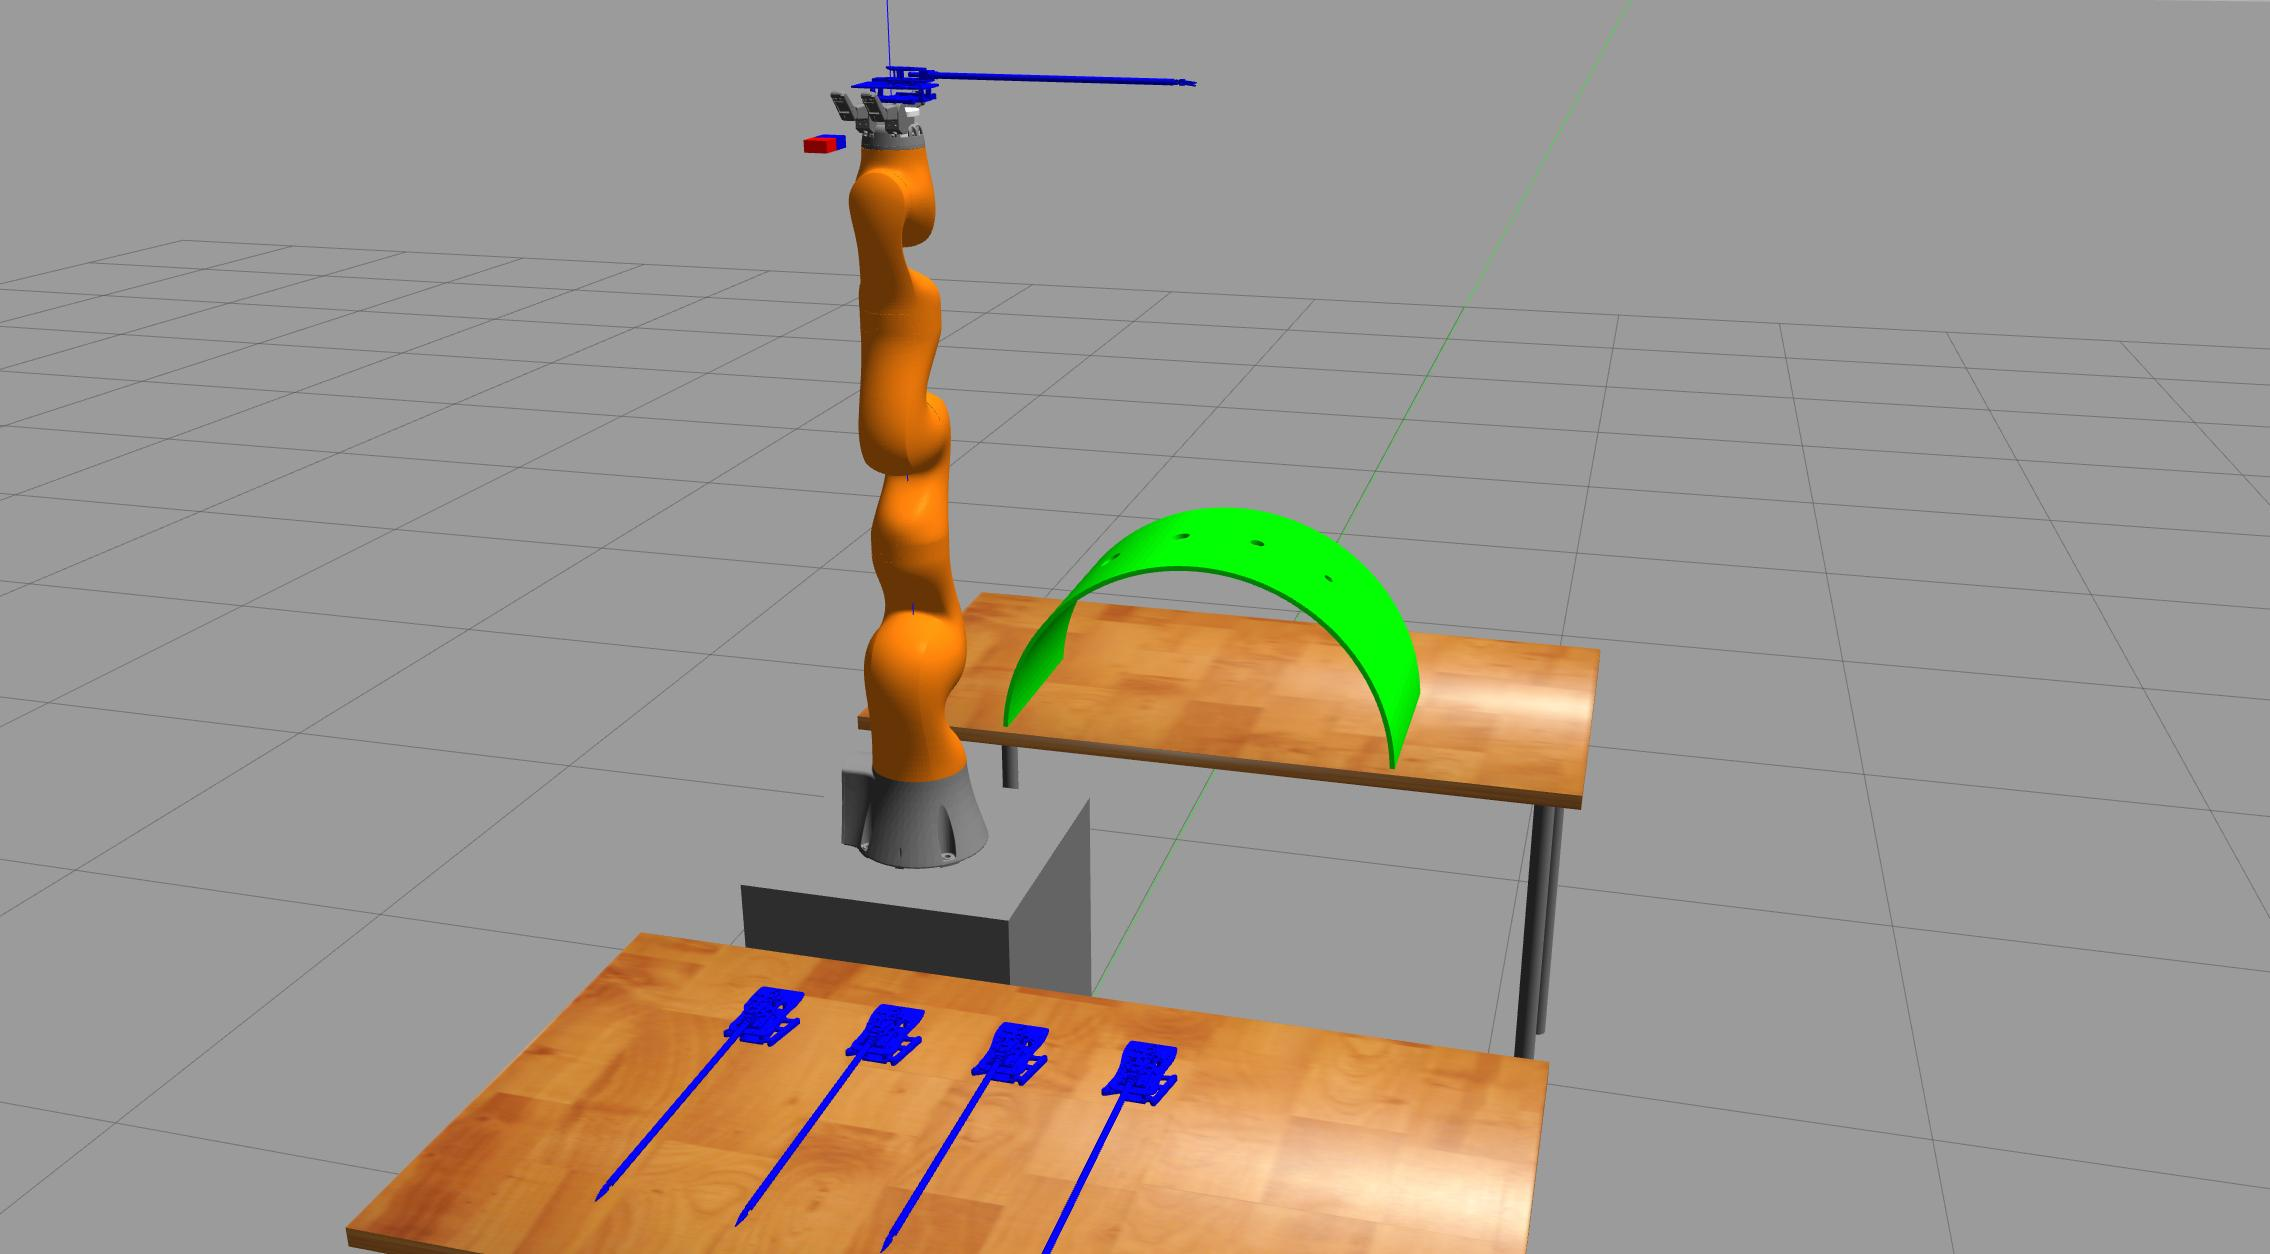
\includegraphics[width=0.3\textwidth]{images/robot_planner1/robot_planner1_1}
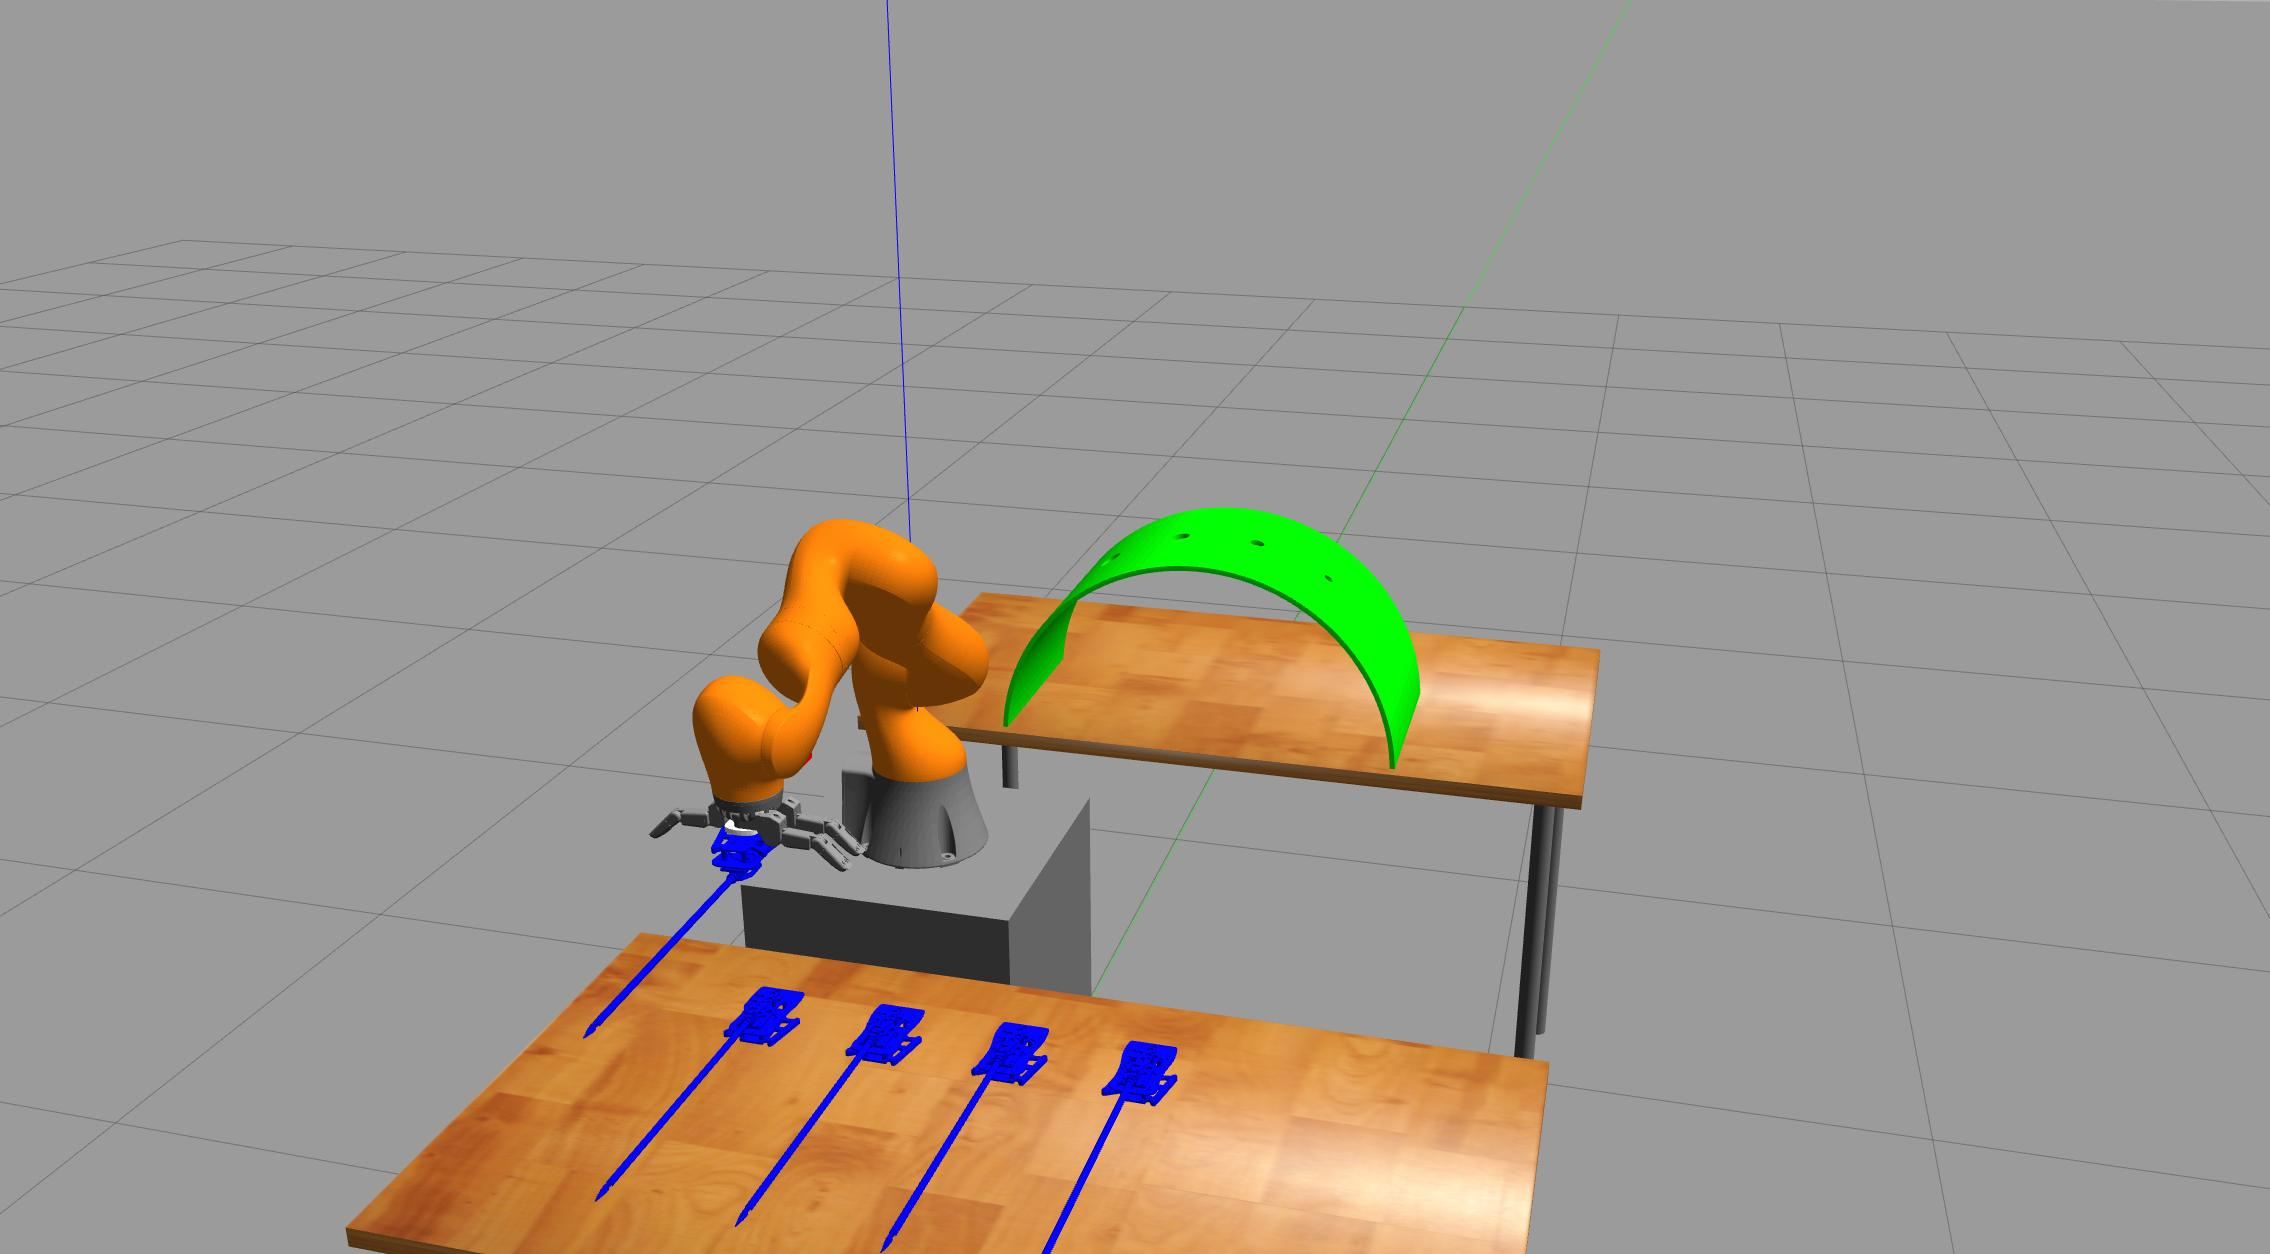
\includegraphics[width=0.3\textwidth]{images/robot_planner1/robot_planner1_2}
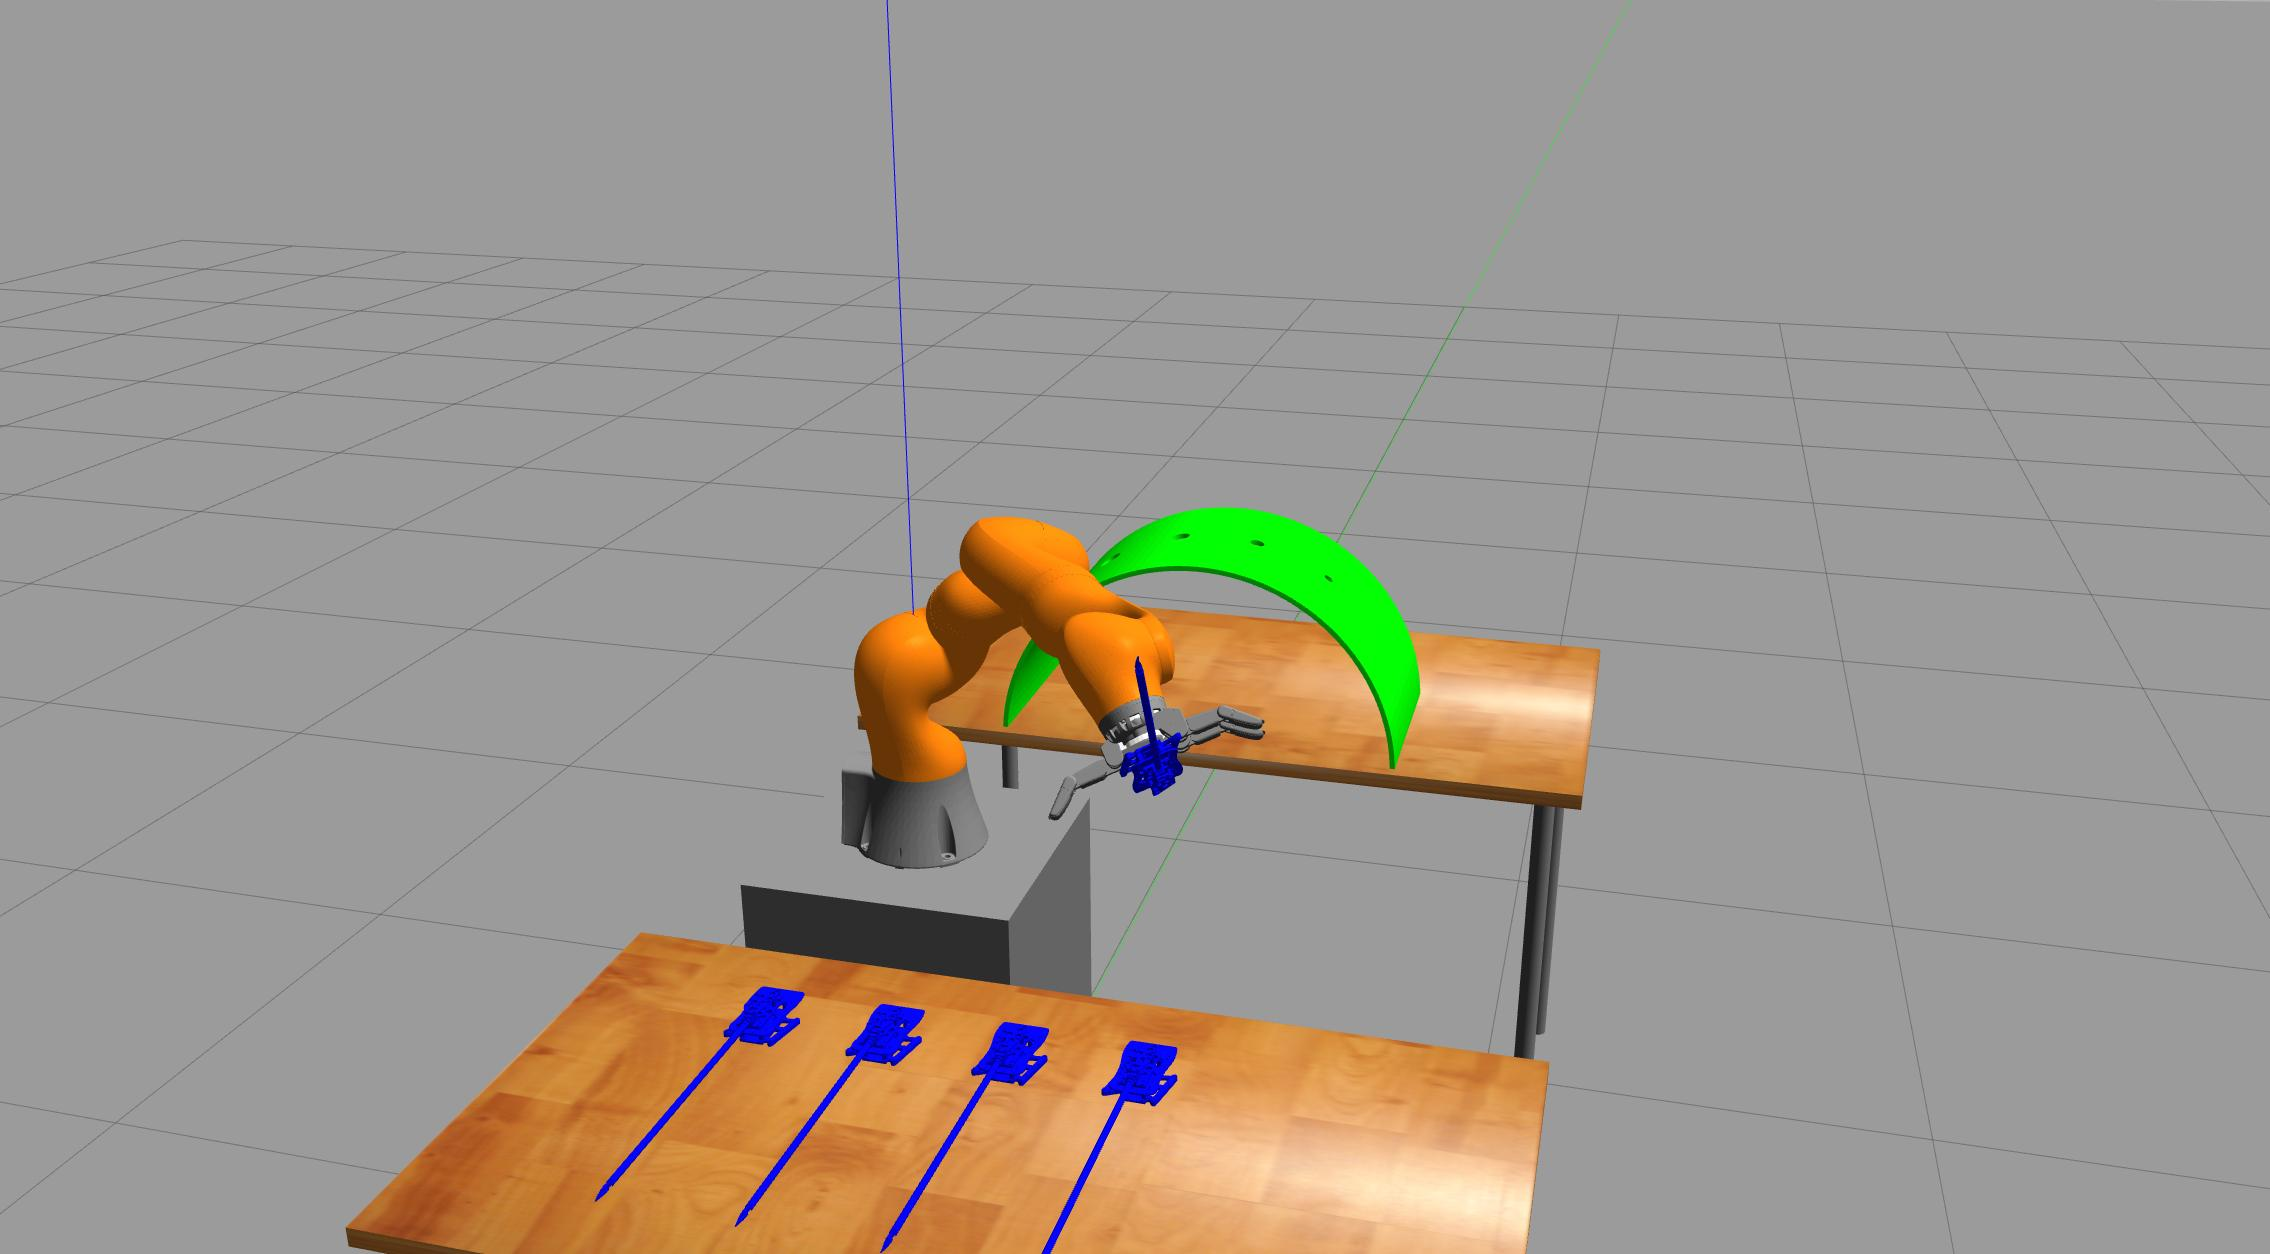
\includegraphics[width=0.3\textwidth]{images/robot_planner1/robot_planner1_3}\\
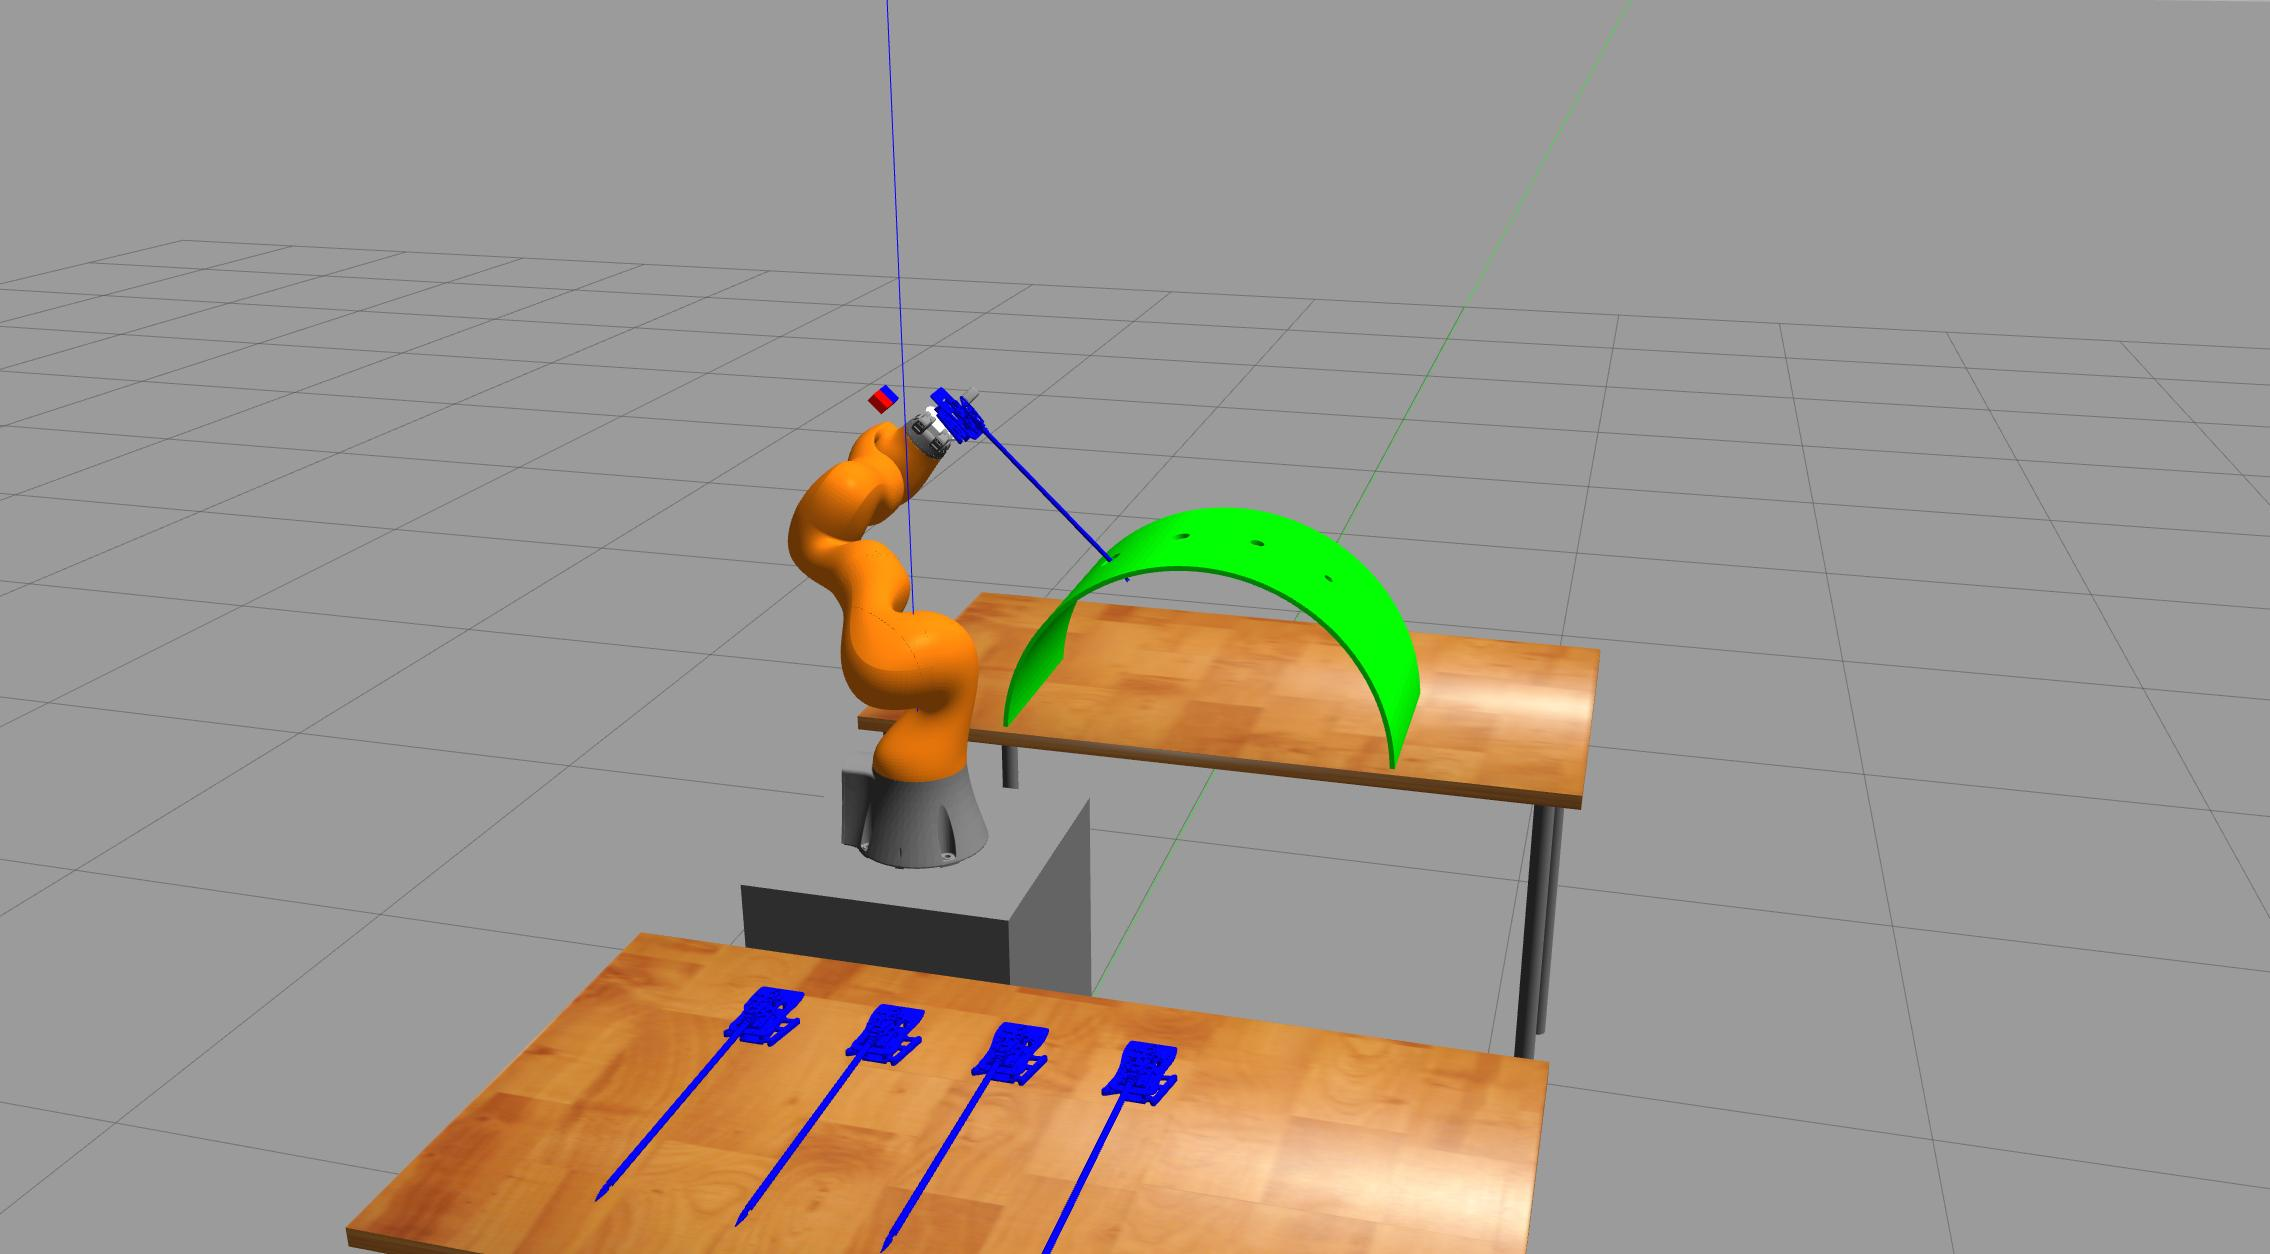
\includegraphics[width=0.3\textwidth]{images/robot_planner1/robot_planner1_4}
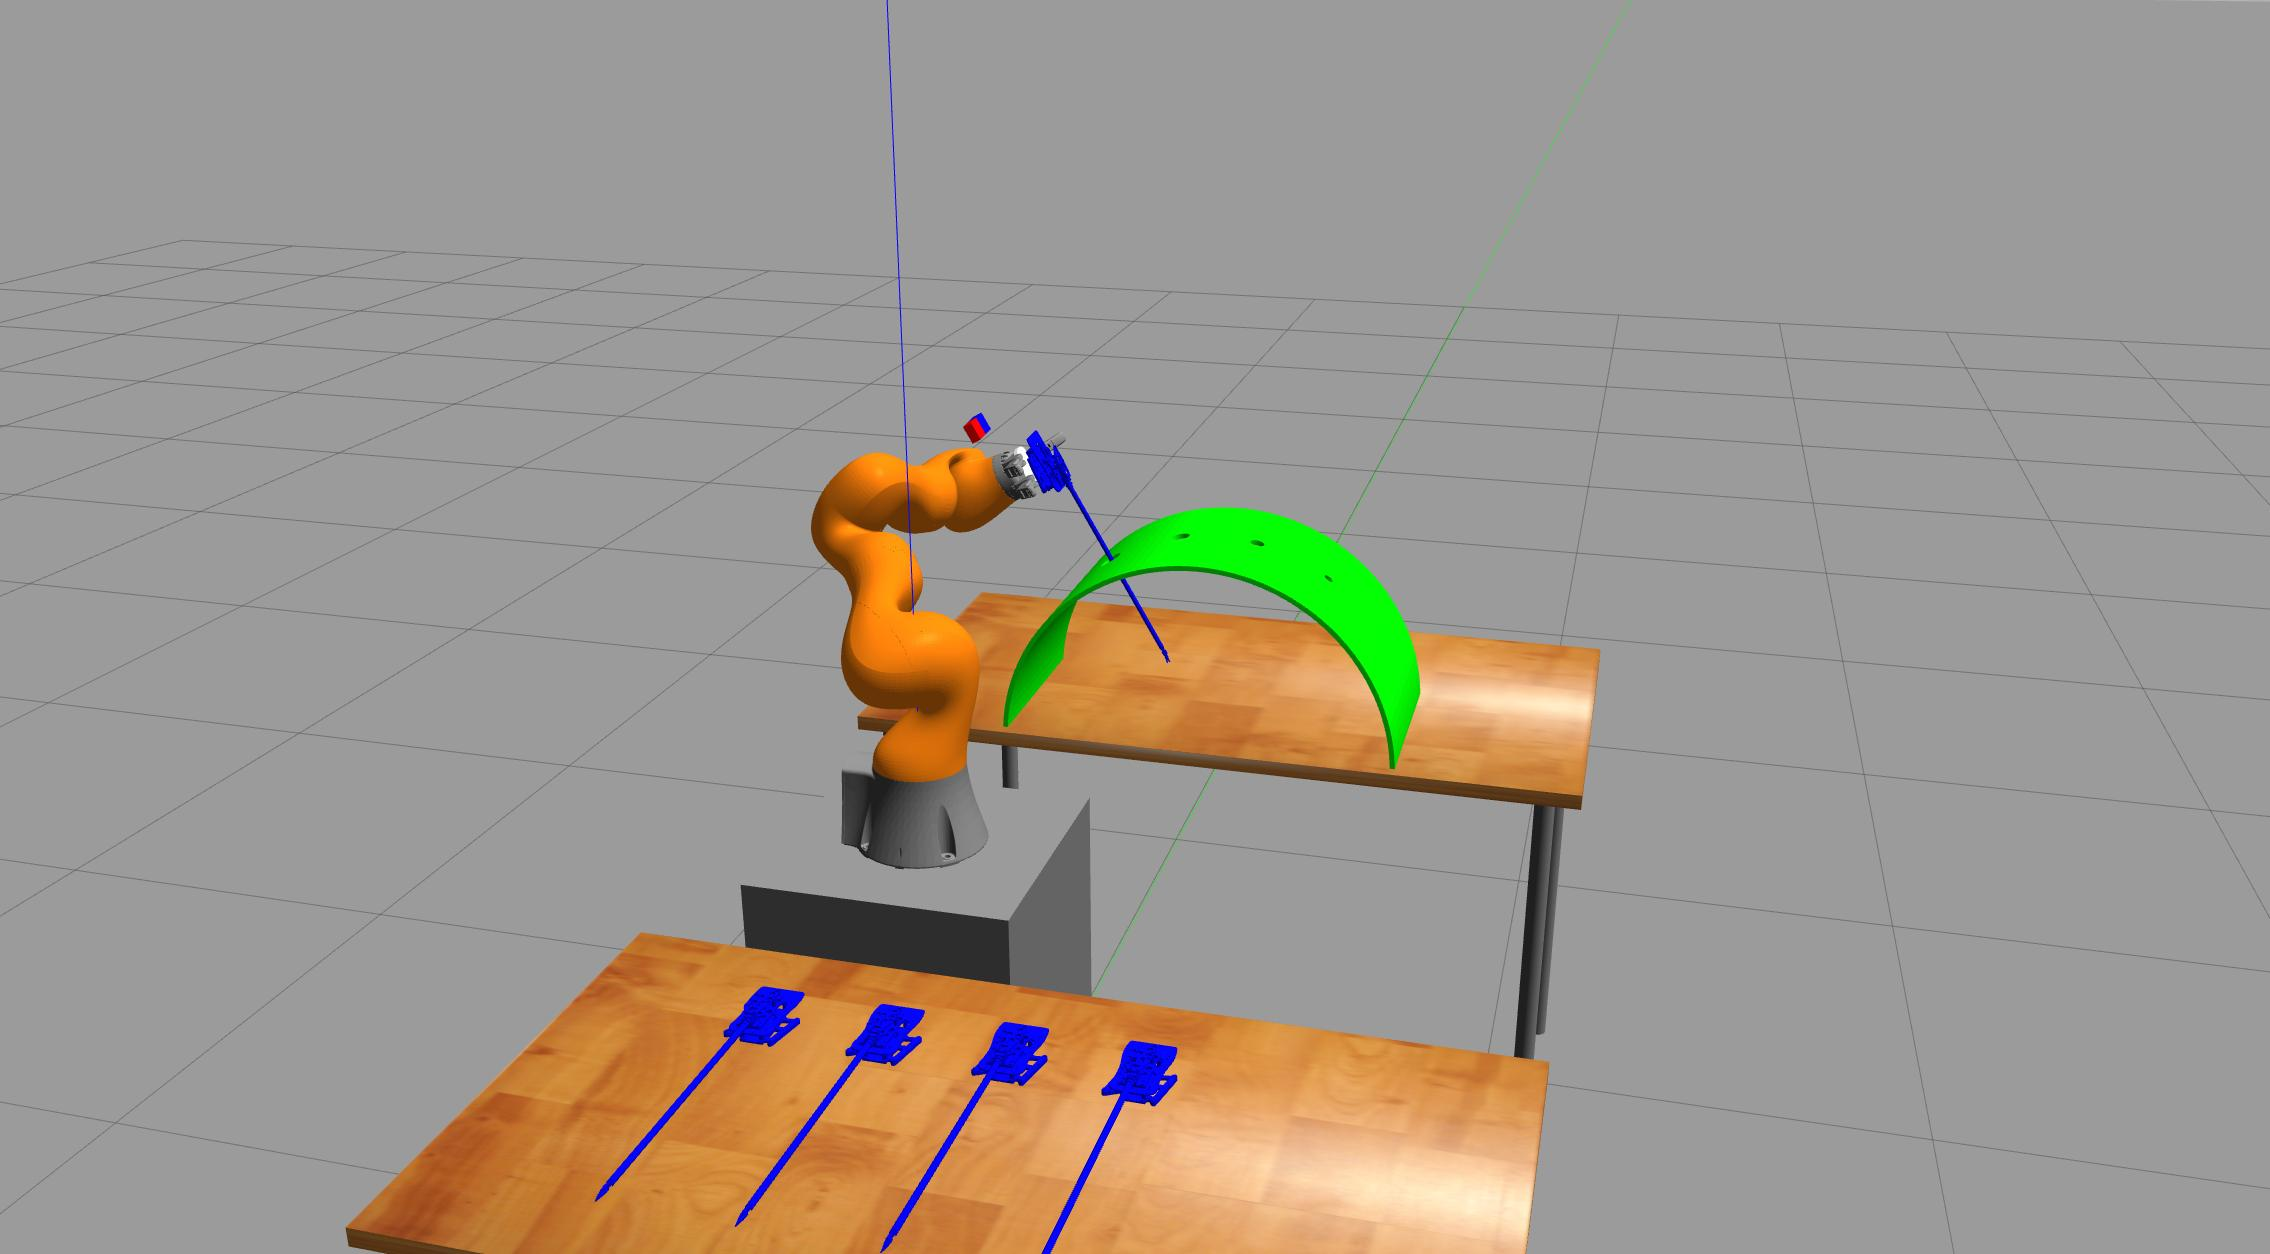
\includegraphics[width=0.3\textwidth]{images/robot_planner1/robot_planner1_5}
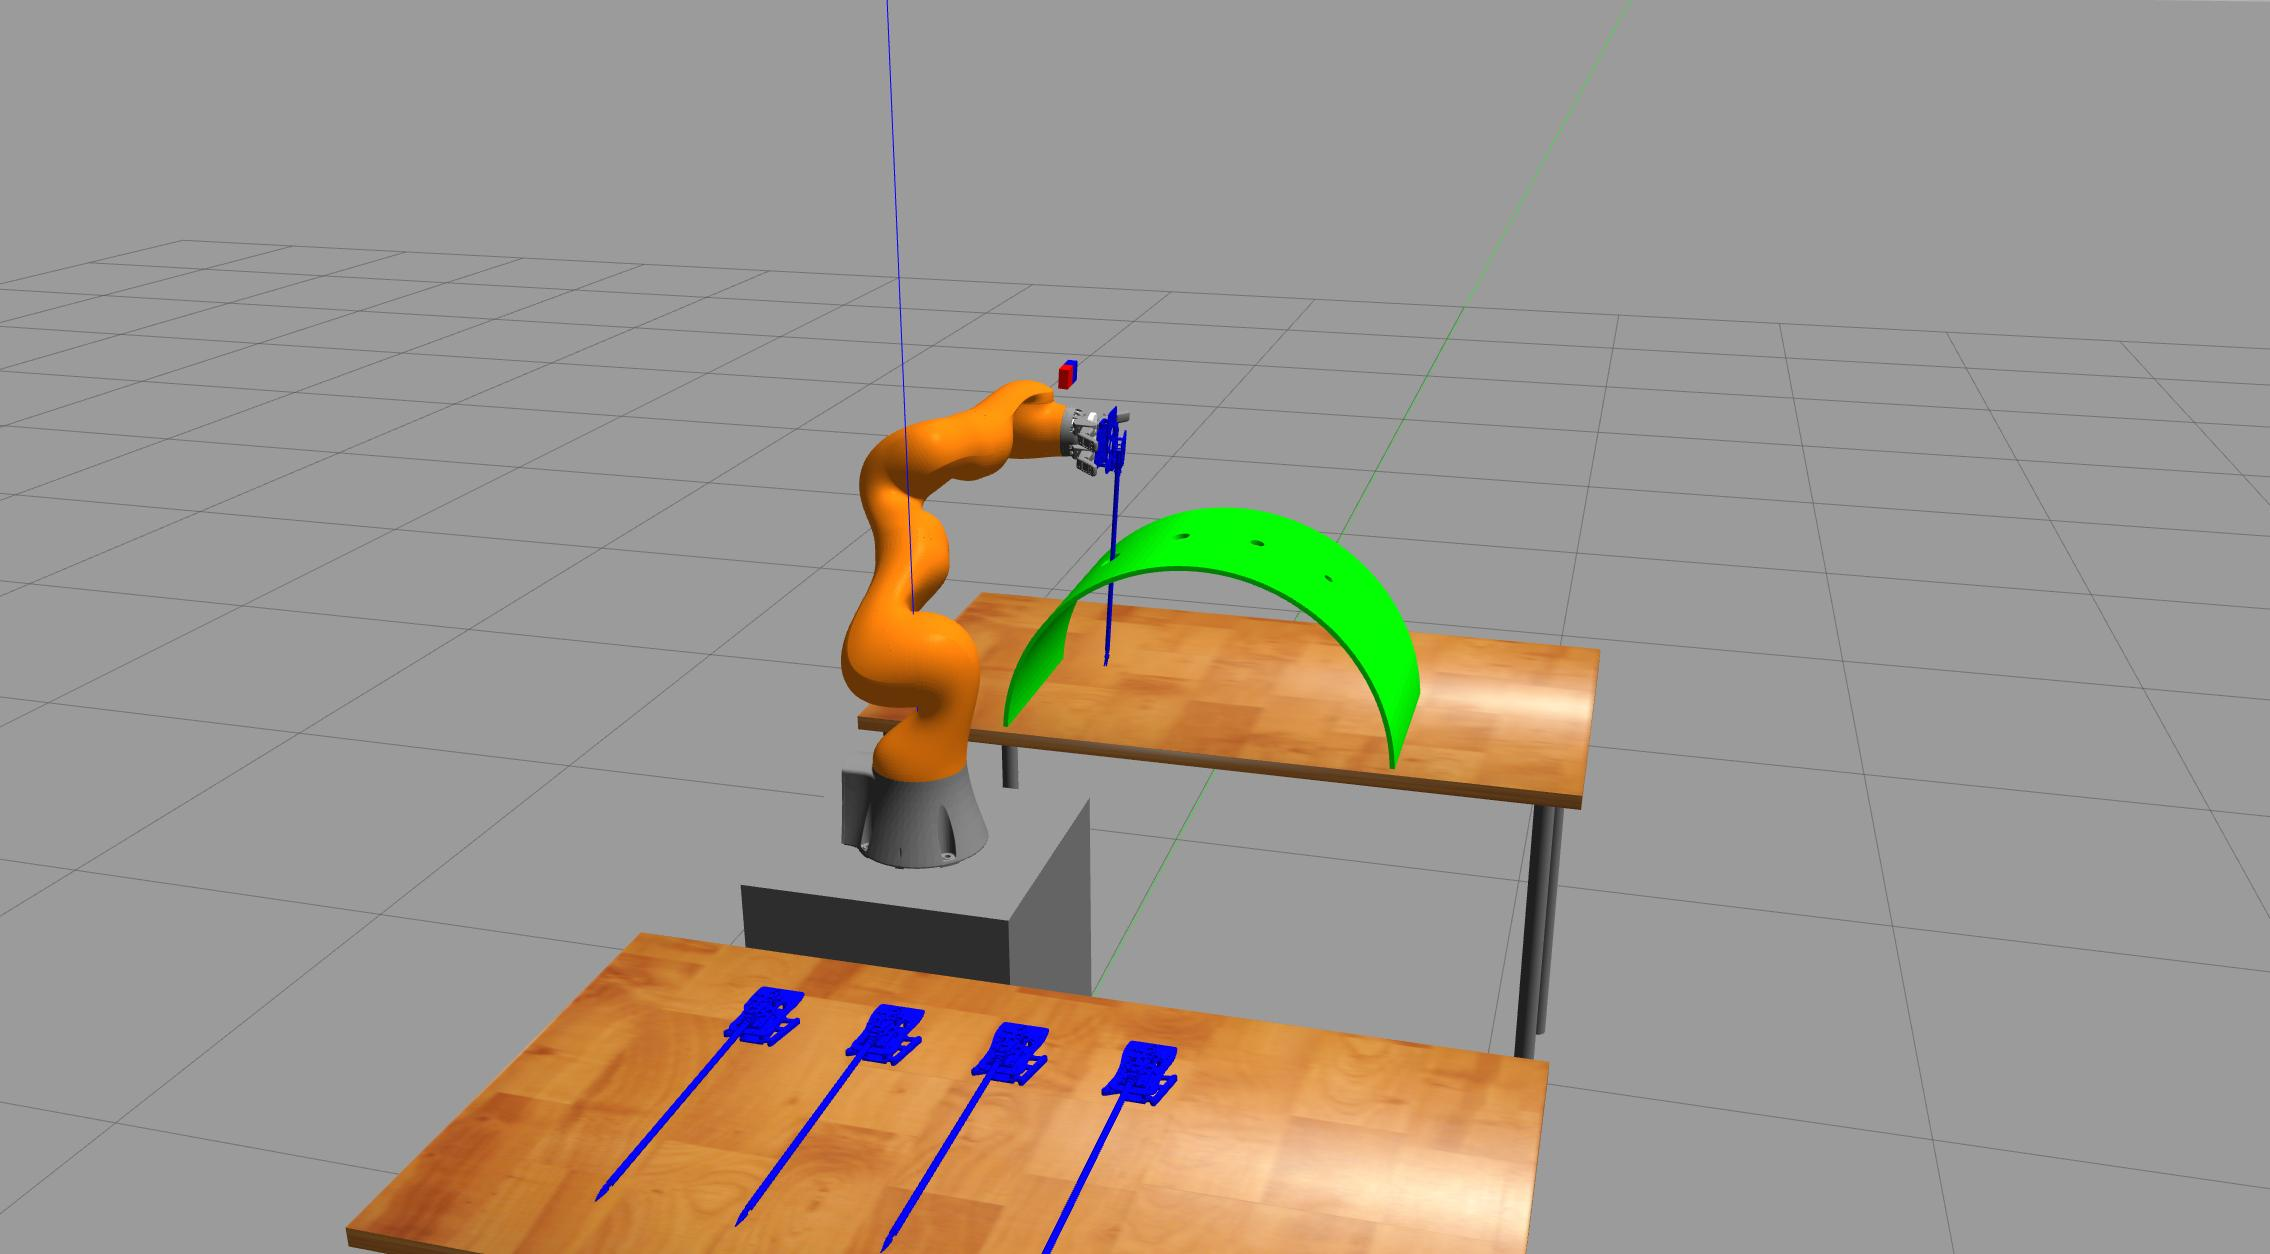
\includegraphics[width=0.3\textwidth]{images/robot_planner1/robot_planner1_6}\\
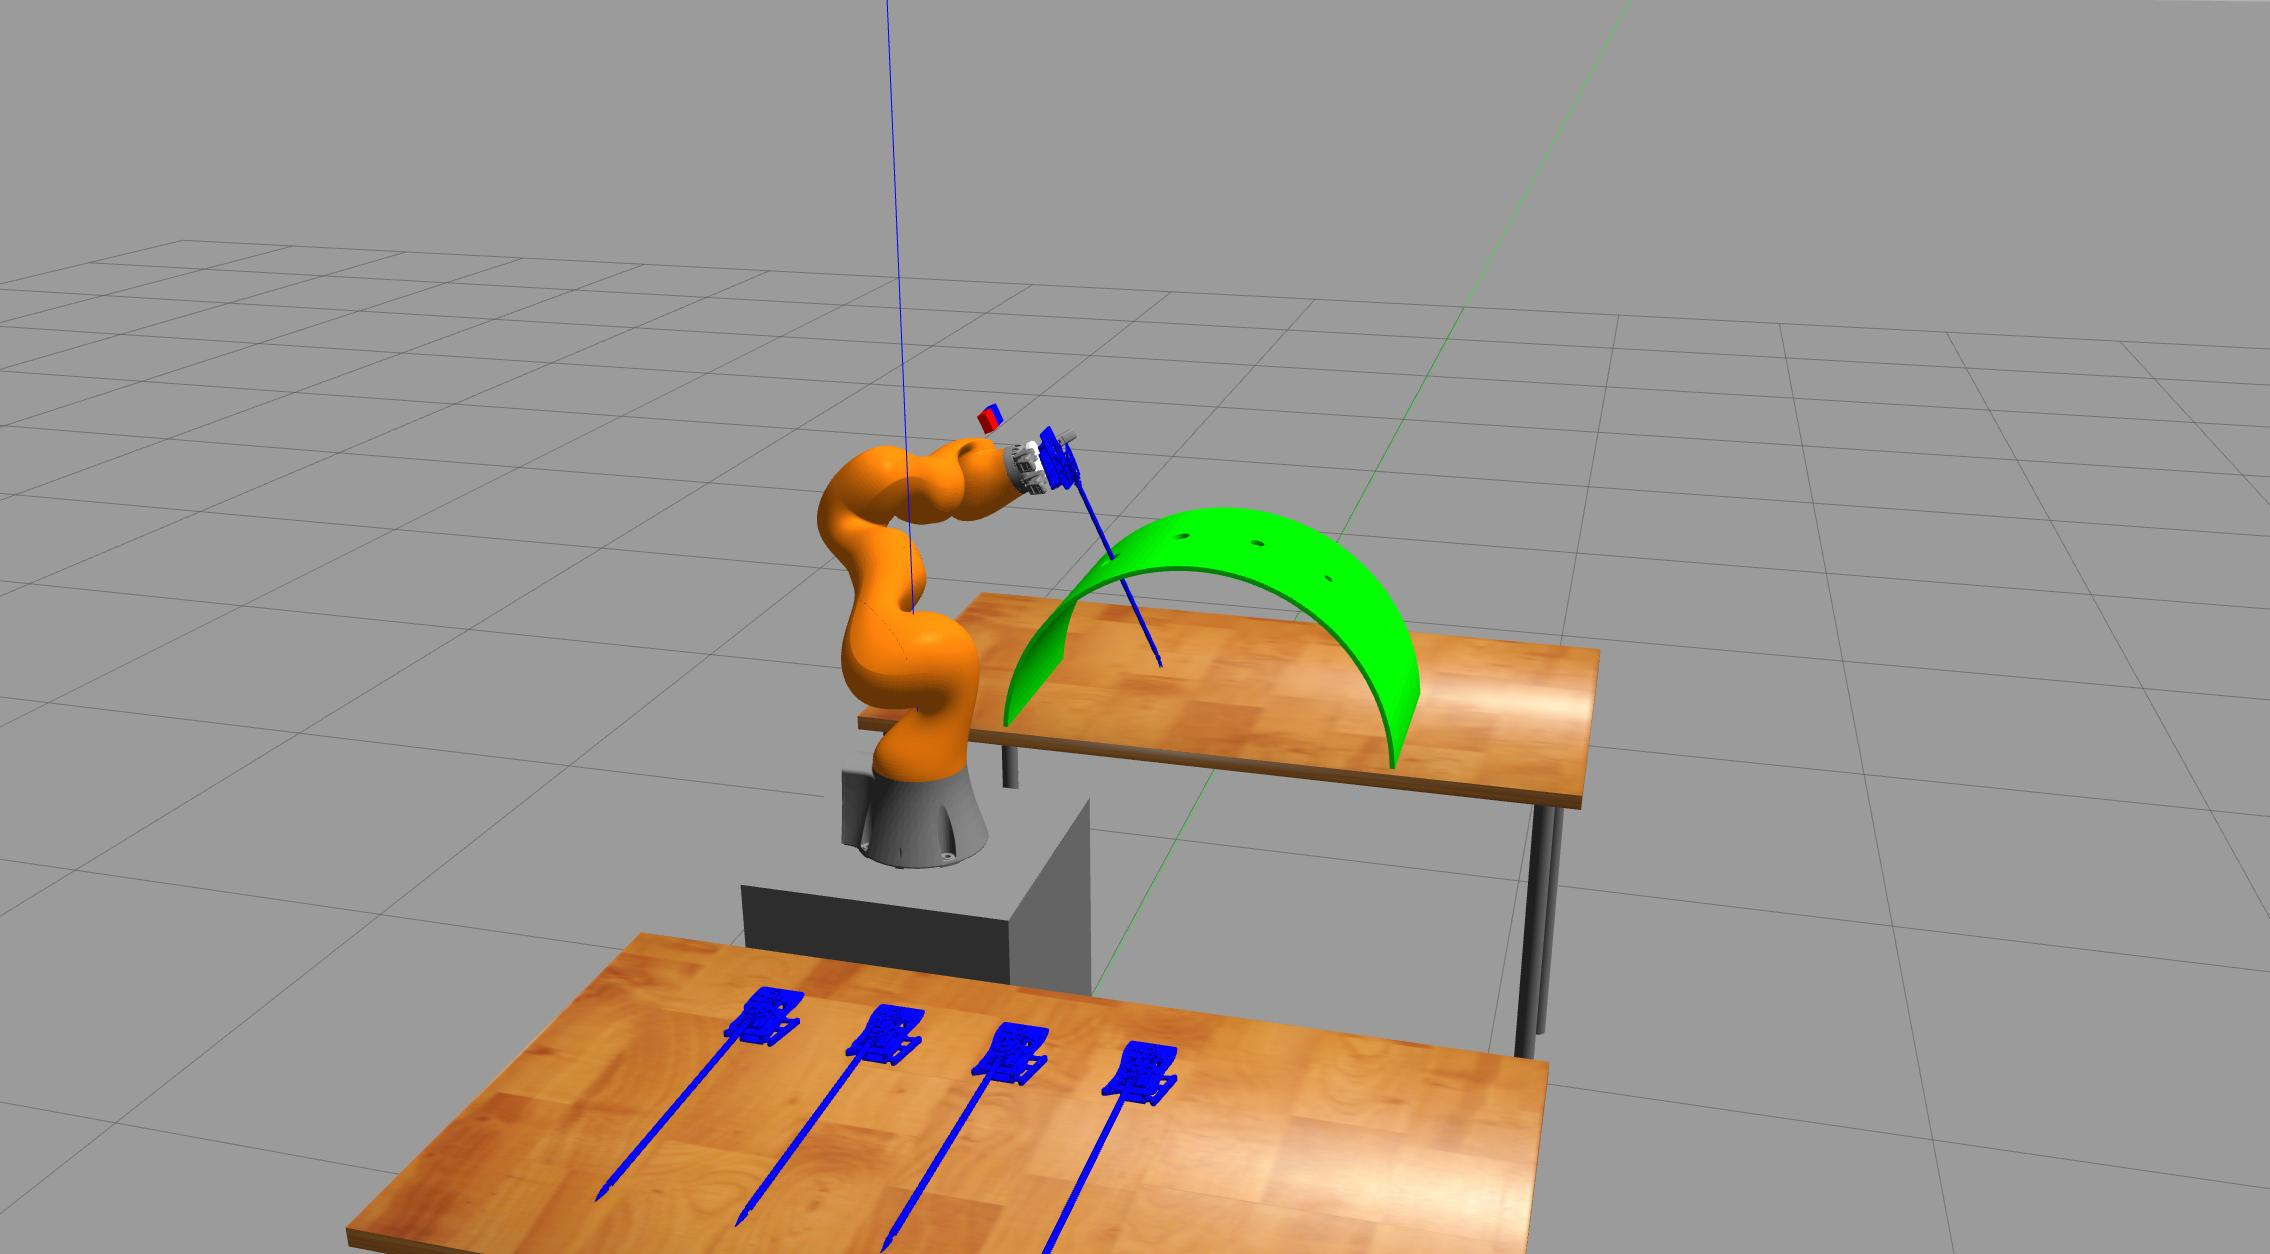
\includegraphics[width=0.3\textwidth]{images/robot_planner1/robot_planner1_7}
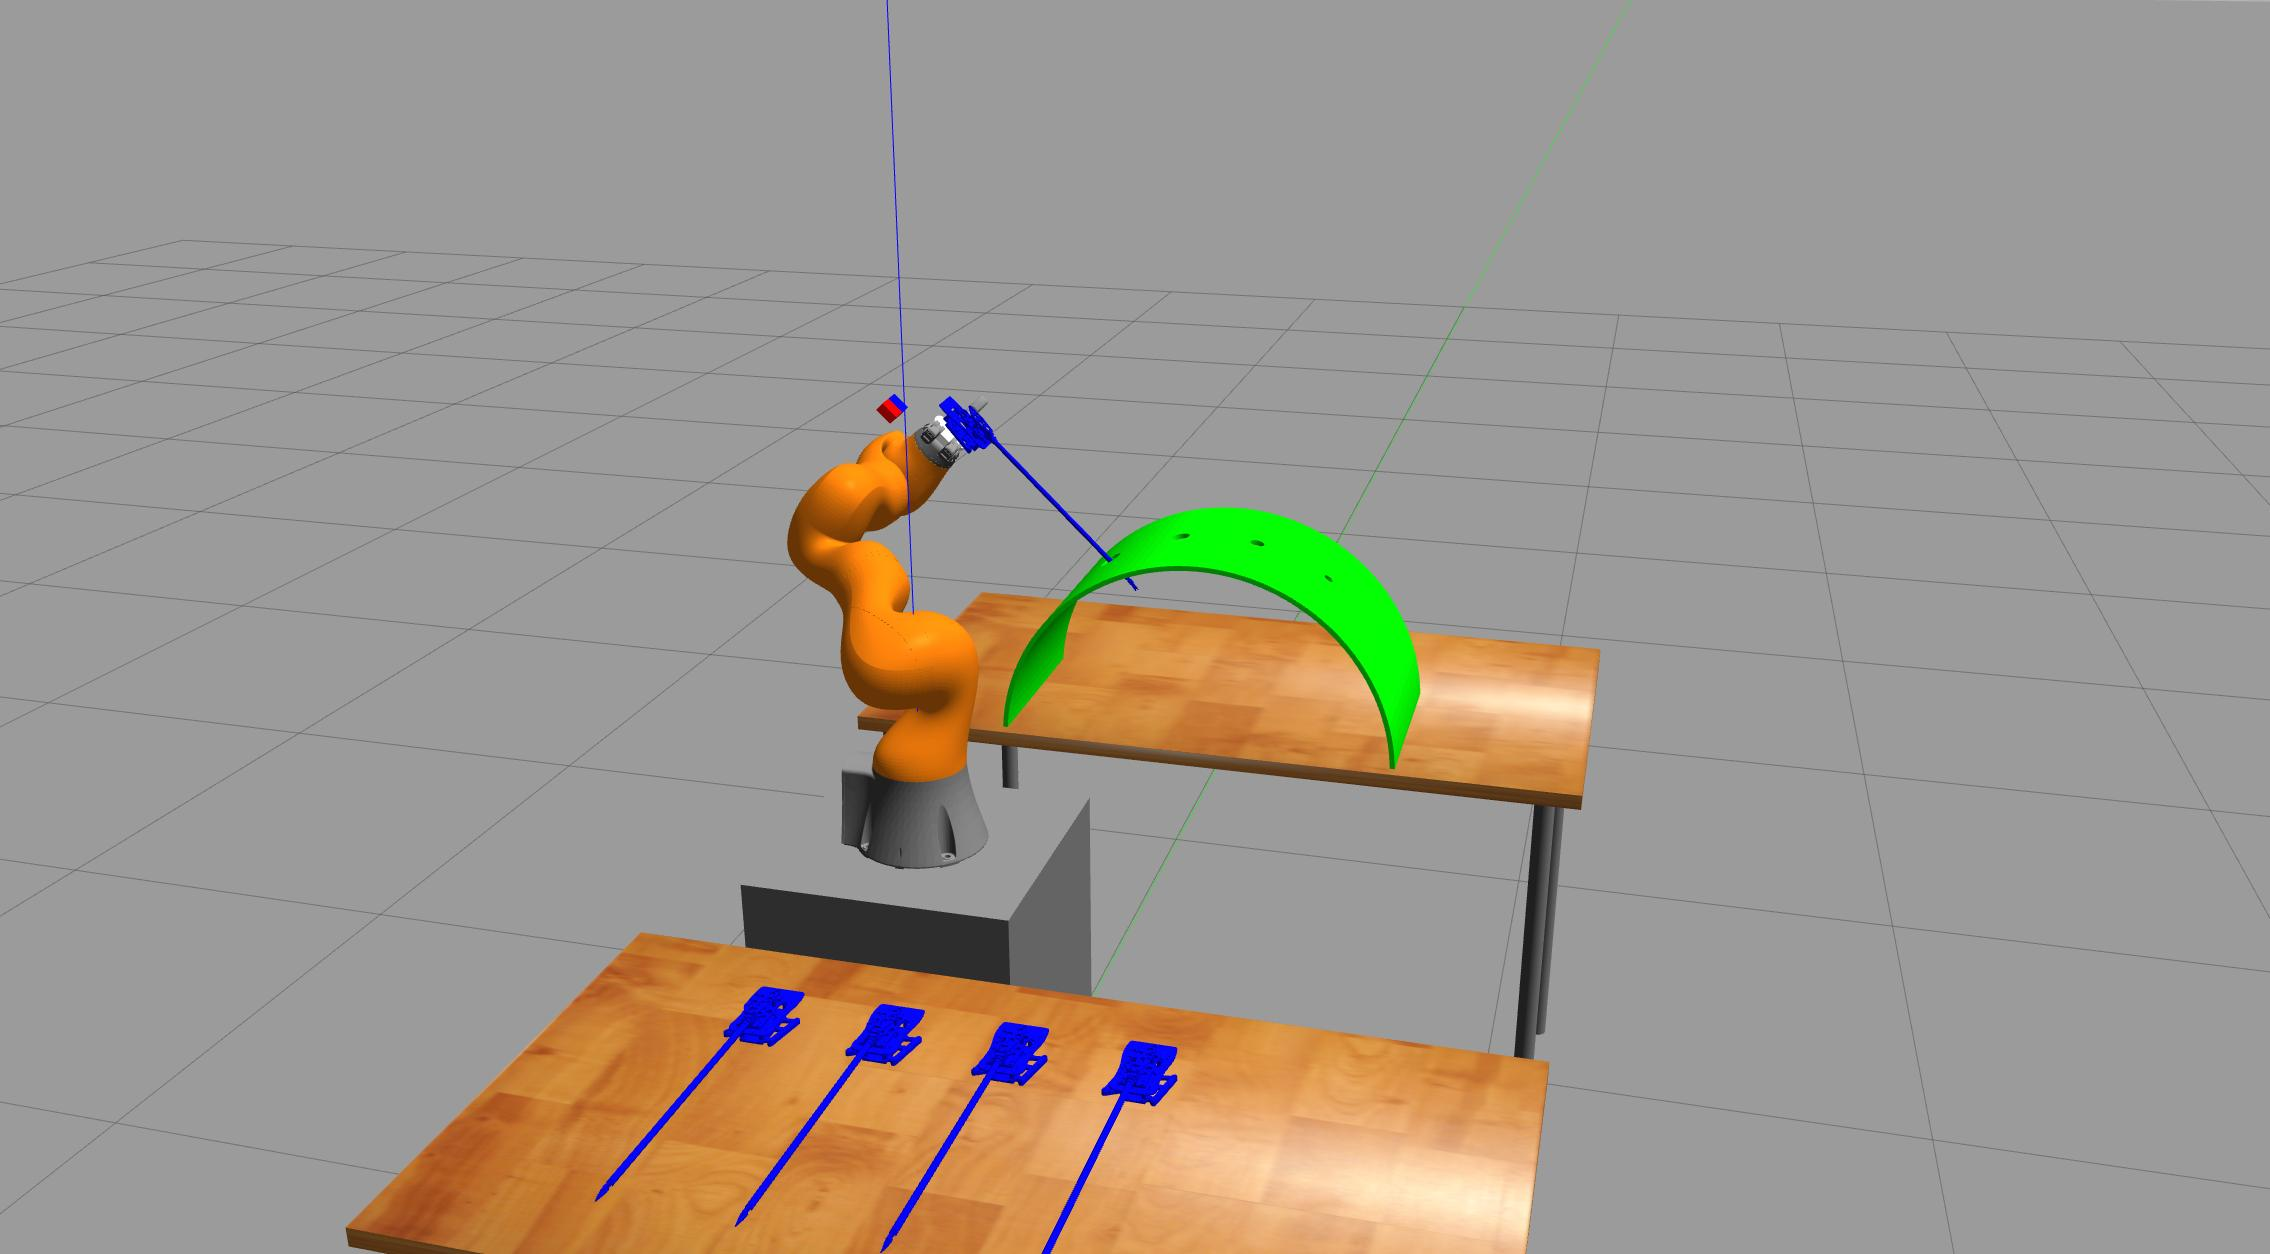
\includegraphics[width=0.3\textwidth]{images/robot_planner1/robot_planner1_8}
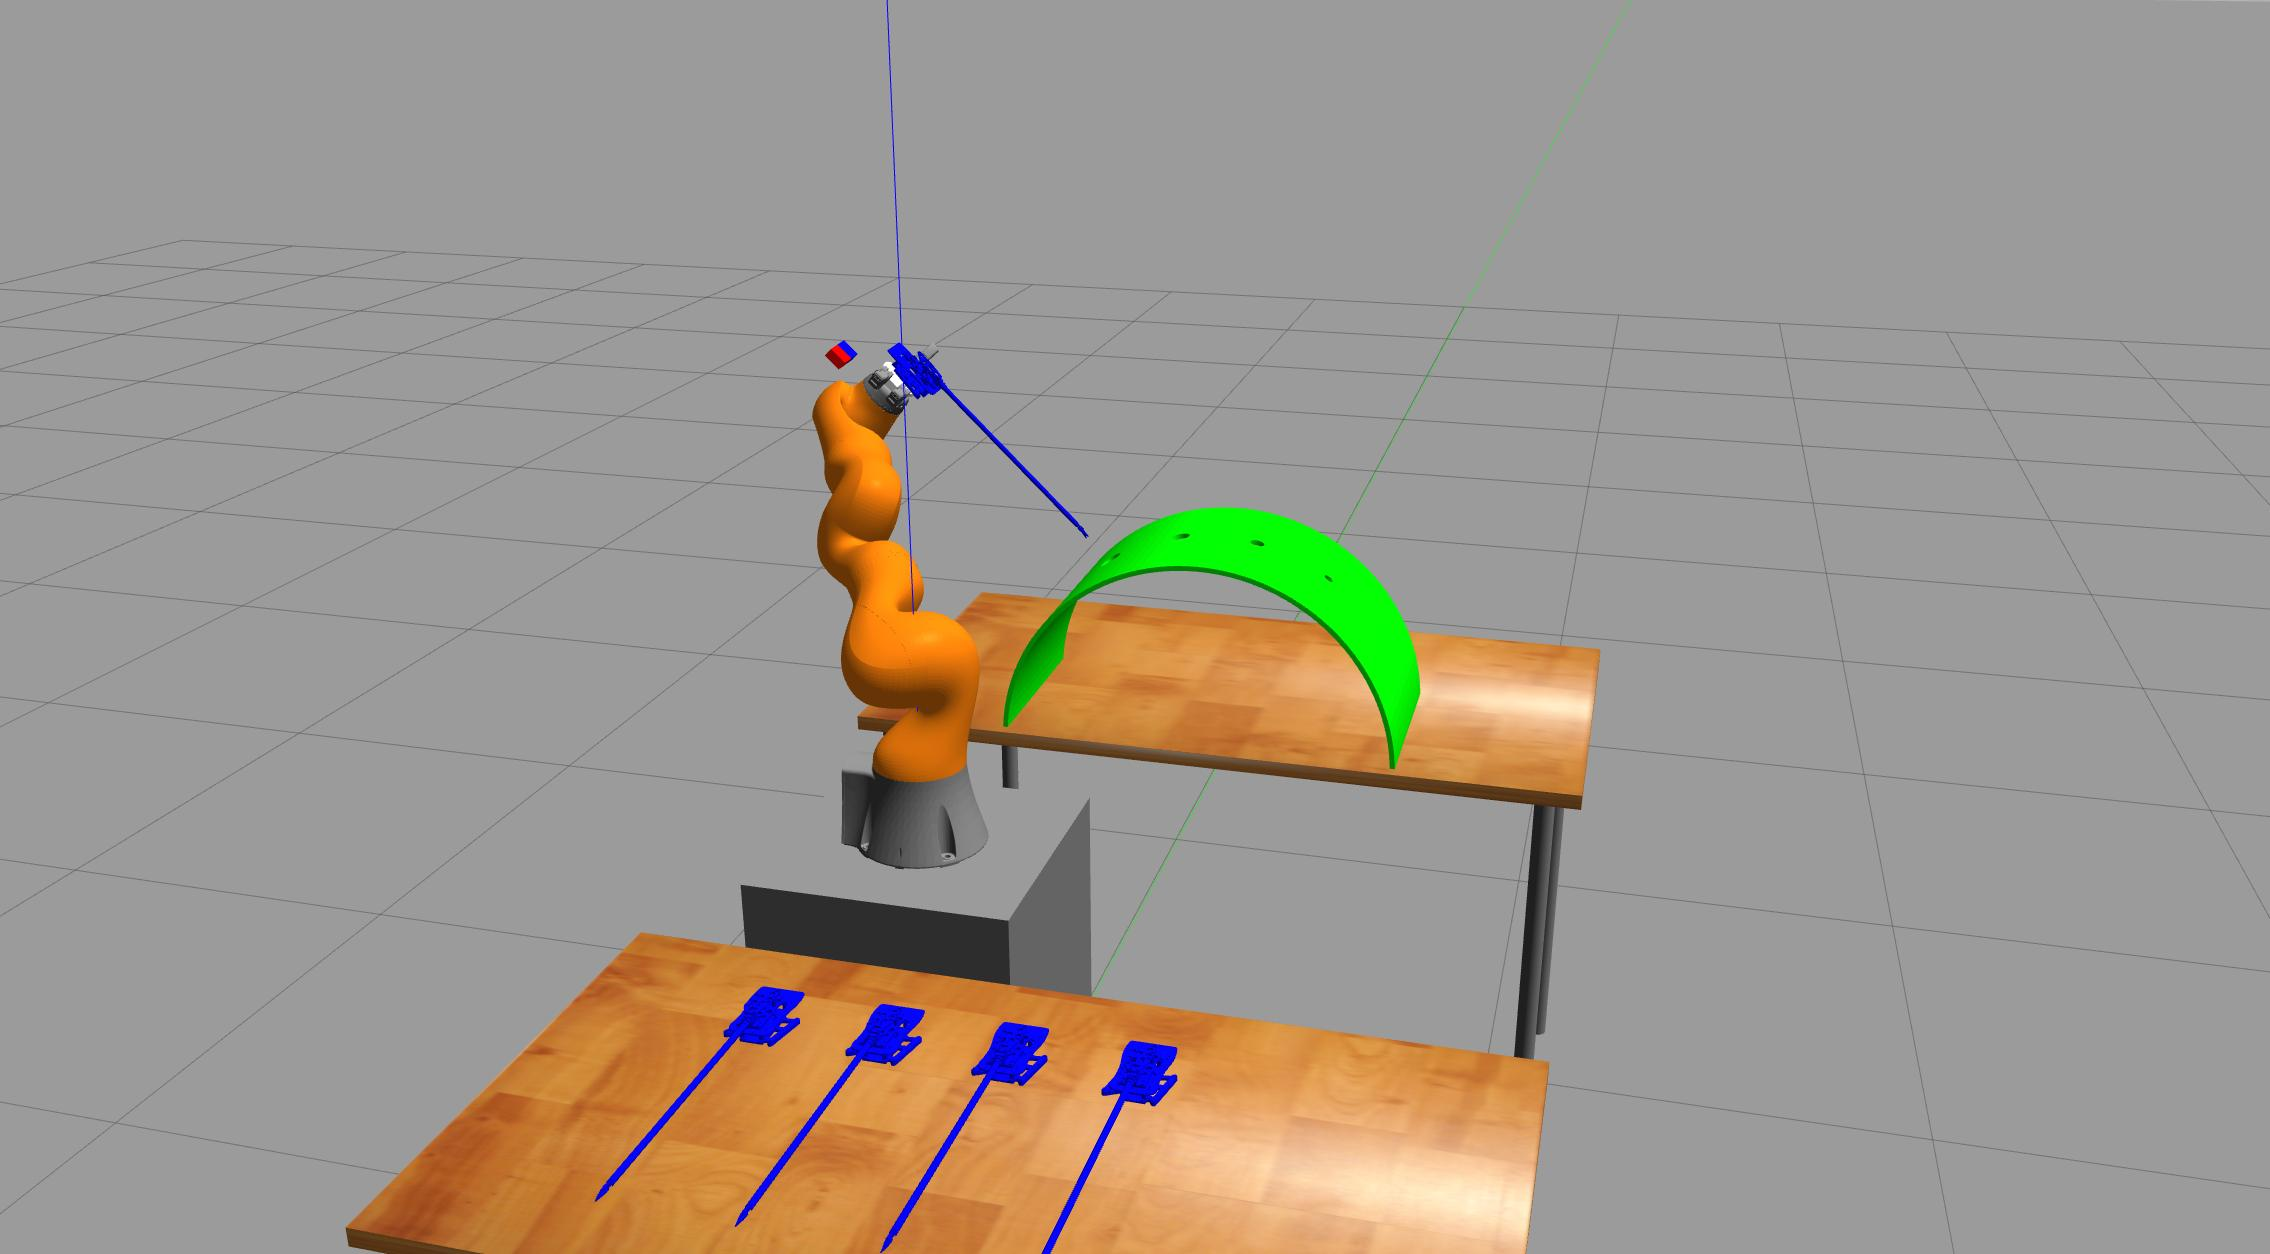
\includegraphics[width=0.3\textwidth]{images/robot_planner1/robot_planner1_9}\\
\caption{Experiment 1:}
\end{figure}
\end{center}

% Robot Planner 1 with RRTConnect
\begin{table}[H]
\centering
\begin{tabular}{|p{2cm}|c|p{2cm}|p{2cm}|p{2cm}|}
\hline
Robot Planner 1           & \multicolumn{4}{c}{\textbf{RRTConnect}}                                                                                                 \vline \\
\hline
                          & \multicolumn{4}{c}{\textbf{Fake tool picking trajectory}}                     \vline \\
\hline
Experiment                & Approach planning time & Execution status & Move away planning time & Execution status  \\
\hline
1 &	0.060402 &	1 &	0.144881 &	1 \\
2 &	0.06053 &	1 &	0.058341 &	1 \\
3 &	0.064706 &	1 &	0.060981 &	1 \\
4 &	0.059789 &	1 &	0.119351 &	1 \\
5 &	0.164789 &	1 &	0.330373 &	1 \\
6 &	0.147037 &	1 &	0.289805 &	1 \\
7 &	0.18233 &	1 &	0.093362 &	1 \\
8 &	0.054469 &	1 &	0.062209 &	1 \\
9 &	0.05313 &	1 &	0.409191 &	1 \\
10 &	0.105909 &	1 &	0.307963 &	1 \\
\hline
\textbf{Average} & 	0.0953091 &	1	& 0.1876457	& 1 \\
\hline
                          & \multicolumn{4}{c}{\textbf{Insertion \& Pivot trajectories}}                     \vline \\
\hline
Experiment                & Insertion planning time & Execution status & Pivot planning time & Execution status  \\
\hline
1	& 0.216565	& 1	& 3.639193	& 1 \\
2	& 0.057143	& 1	& 0.057187	& 1 \\
3	& 0.073242	& 1	& 0.072451	& 1 \\
4	& 0.056255	& 1	& 0.068156	& 1 \\
5	& 0.16178	& 1	& 0.150123	& 1 \\
6	& 0.071426	& 1	& 0.065059	& 1 \\
7	& 0.155125	& 1	& -	& 0 \\
8	& 0.315921	& 1	& 0.194663	& 1 \\
9	& 0.127381	& 1	& 0.19026	& 1 \\
10	& 0.396182	& 1	& 0.075866	& 1 \\
\hline
\textbf{Average} & 	0.163102 & 1	& 0.5014398 &	0.9 \\
\hline
                          & \multicolumn{4}{c}{\textbf{Reverse pivot \& reverse insertion trajectories}}                     \vline \\
\hline
Experiment                & Reverse pivot planning time & Execution status & Reverse insertion planning time & Execution status  \\
\hline
1 & 2.419514	& 1	& 2.388166	& 1 \\
2 & 1.386188	& 1	& 2.874223	& 0 \\
3 & -	& 0	& 5.106926	& 1 \\
4 & 5.466561	& 1	& 4.562506	& 1 \\
5 & 5.62329	& 1	& 5.587679	& 1 \\
6 & 5.488728	& 0	& -	& 0 \\
7 & -	& 0	& -	& 0 \\
8 & -	& 0	& -	& 0 \\
9 & 5.291442	& 1	& 5.096234	& 1 \\
10 & 5.381595	& 1	& 5.576362	& 1 \\
\hline
\textbf{Average} & 	4.436760	& 0.6	& 4.456014	& 0.6 \\
\hline
\end{tabular}
\caption{Time results for robot planner 1 using the RRTConnect path planner algorithm. Planning time is the sum of solution time and path simplification time. Execution status is 
1 for success and 0 for failure. Parameters: tolerances: 0.000005, max planning time: 5 seconds, replanning: true, max planning attempts: 6. Experiments start from home position.}
\label{robot-planner1-rrtconnect-data}
\end{table}


% Robot Planner 1 with RRT*
\begin{table}[H]
\centering
\begin{tabular}{|p{2cm}|c|p{2cm}|p{2cm}|p{2cm}|}
\hline
Robot Planner 1           & \multicolumn{4}{c}{\textbf{RRT*}}                                                                                                 \vline \\
\hline
                          & \multicolumn{4}{c}{\textbf{Fake tool picking trajectory}}                     \vline \\
\hline
Experiment                & Approach planning time & Execution status & Move away planning time & Execution status  \\
\hline
1	& 5.096772	& 1	& 5.023175	& 1 \\
2	& 5.015857	& 1	& 5.034447	& 1 \\
3	& 5.01843	& 1	& 5.101766	& 1 \\
4	& 5.074703	& 1	& 5.089464	& 1 \\
5	& 5.019108	& 1	& 5.056875	& 1 \\
6	& 5.011631	& 1	& 5.217069	& 1 \\
7	& 5.119638	& 1	& 5.027692	& 1 \\
8	& 5.121159	& 1	& 5.040244	& 1 \\
9	& 5.12812	& 1	& 5.098381	& 1 \\
10	& 5.343964	& 1	& 5.374314	& 1 \\
\hline
\textbf{Average} & 	5.0949382	& 1	& 5.1063427	& 1 \\
\hline
                          & \multicolumn{4}{c}{\textbf{Insertion \& Pivot trajectories}}                     \vline \\
\hline
Experiment                & Insertion planning time & Execution status & Pivot planning time & Execution status  \\
\hline
1 & 5.200983  & 1 &  5.044568 &  1 \\
2 & 5.009846  & 1 &  -  &  0 \\
3 & 5.064216  & 1 &  5.085314 &  1 \\
4 & 5.145115  & 1 &  5.059245 &  1 \\
5 & 5.019322  & 1 &  5.173925 &  1 \\
6 & 5.015804  & 1 &  -  &  0 \\
7 & 5.033637  & 1 &  -  &  0 \\
8 & 5.159212  & 1 &  5.100395 &  1 \\
9 & 5.134356  & 1 &  5.081432 &  1 \\
10  & 5.052 & 0  & - &  0 \\
\hline
\textbf{Average} & 	5.083449	& 0.9	& 5.090813	& 0.6 \\
\hline
                          & \multicolumn{4}{c}{\textbf{Reverse pivot \& reverse insertion trajectories}}                     \vline \\
\hline
Experiment                & Reverse pivot planning time & Execution status & Reverse insertion planning time & Execution status  \\
\hline
1 & -	& 0	& -	& 0 \\
2 & -	& 0	& -	& 0 \\
3 & -	& 0	& 5.508861	& 1 \\
4 & -	& 1	& 5.417935	& 1 \\
5 & 5.057058	& 1	& 5.093558	& 1 \\
6 & -	& 0	& -	& 0 \\
7 & -	& 0	& -	& 0 \\
8 & -	& 0	& -	& 0 \\
9 & -	& 0	& -	& 0 \\
10  & -	& 0	& 5.358954	& 0 \\
\hline
\textbf{Average} & inconclusive	& 0.2	& inconclusive	& 0.3 \\
\hline
\end{tabular}
\caption{Time results for robot planner 1 using the RRT* path planner algorithm. Planning time is the sum of solution time and path simplification time. Execution status is 
1 for success and 0 for failure. Parameters: tolerances: 0.000005, max planning time: 5 seconds, replanning: true, max planning attempts: 6. Experiments start from home position.}
\label{robot-planner1-rrtstar-data}
\end{table}


\section{Robot Planner 2: Simulation layout and reachability experiments}

In this experiment, we plan a path such that the robot arm will visit all holes of the mounting dock and will try the insertion movement of the surgical tool.
This experiment is very useful, because it shows whether all holes of the mounting dock are \textbf{reachable} (inside the robot's work space) and if so, how 
\textbf{dexterous} the robot will be in pivoting around each hole, i.e. how free the robot arm is to execute pivot motions.

\begin{center}
\begin{figure}[H]
\centering
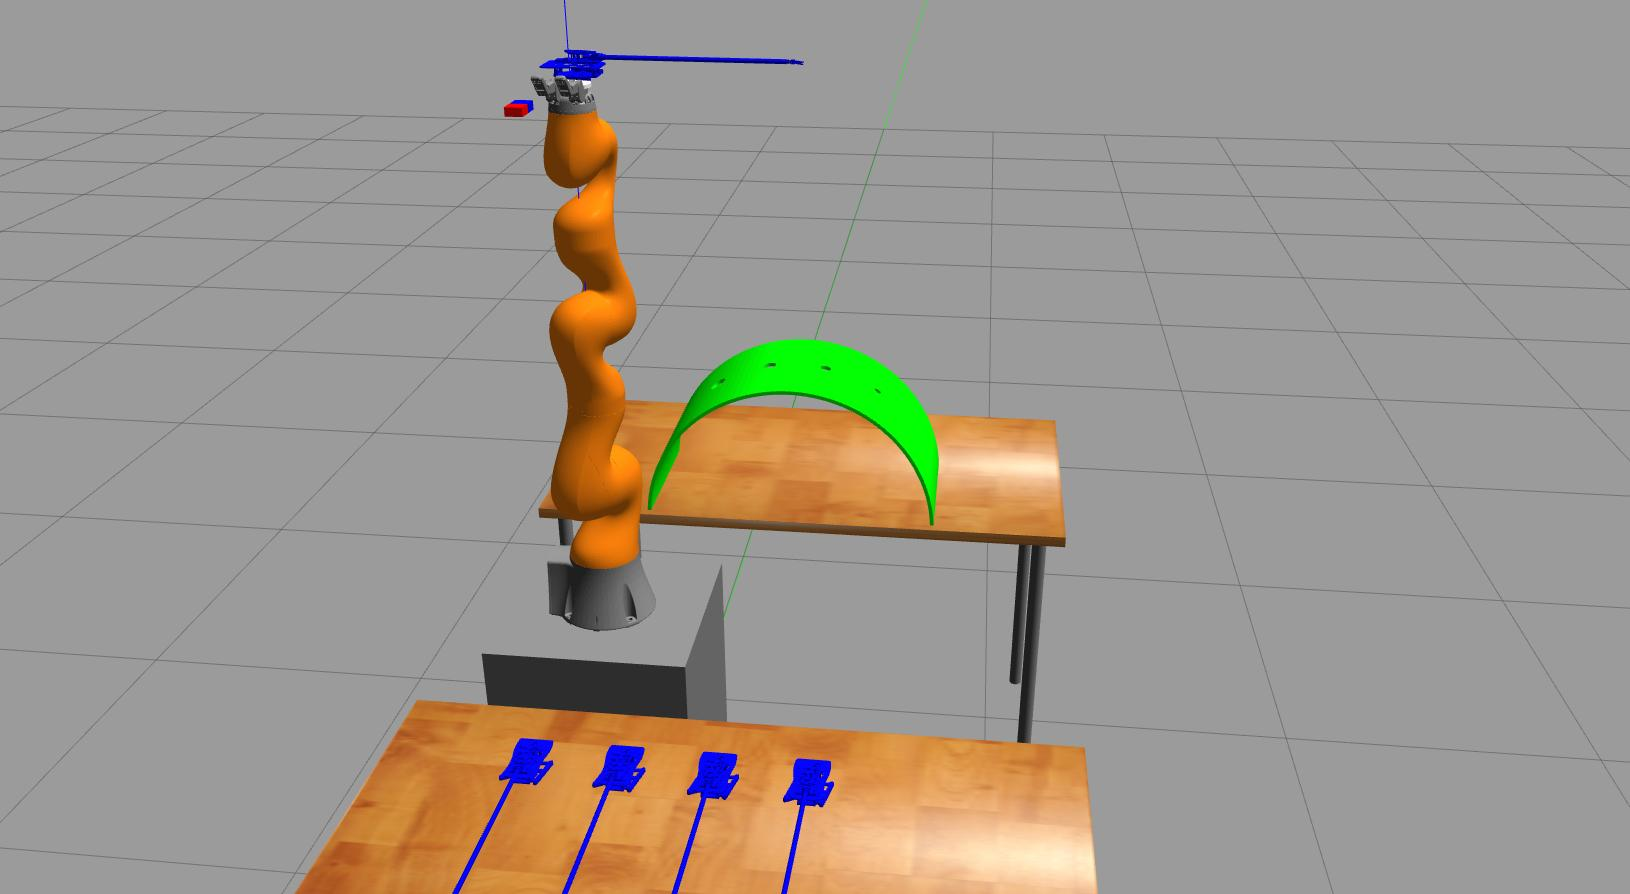
\includegraphics[width=0.31\textwidth]{images/robot_planner2/robot_planner2_1}
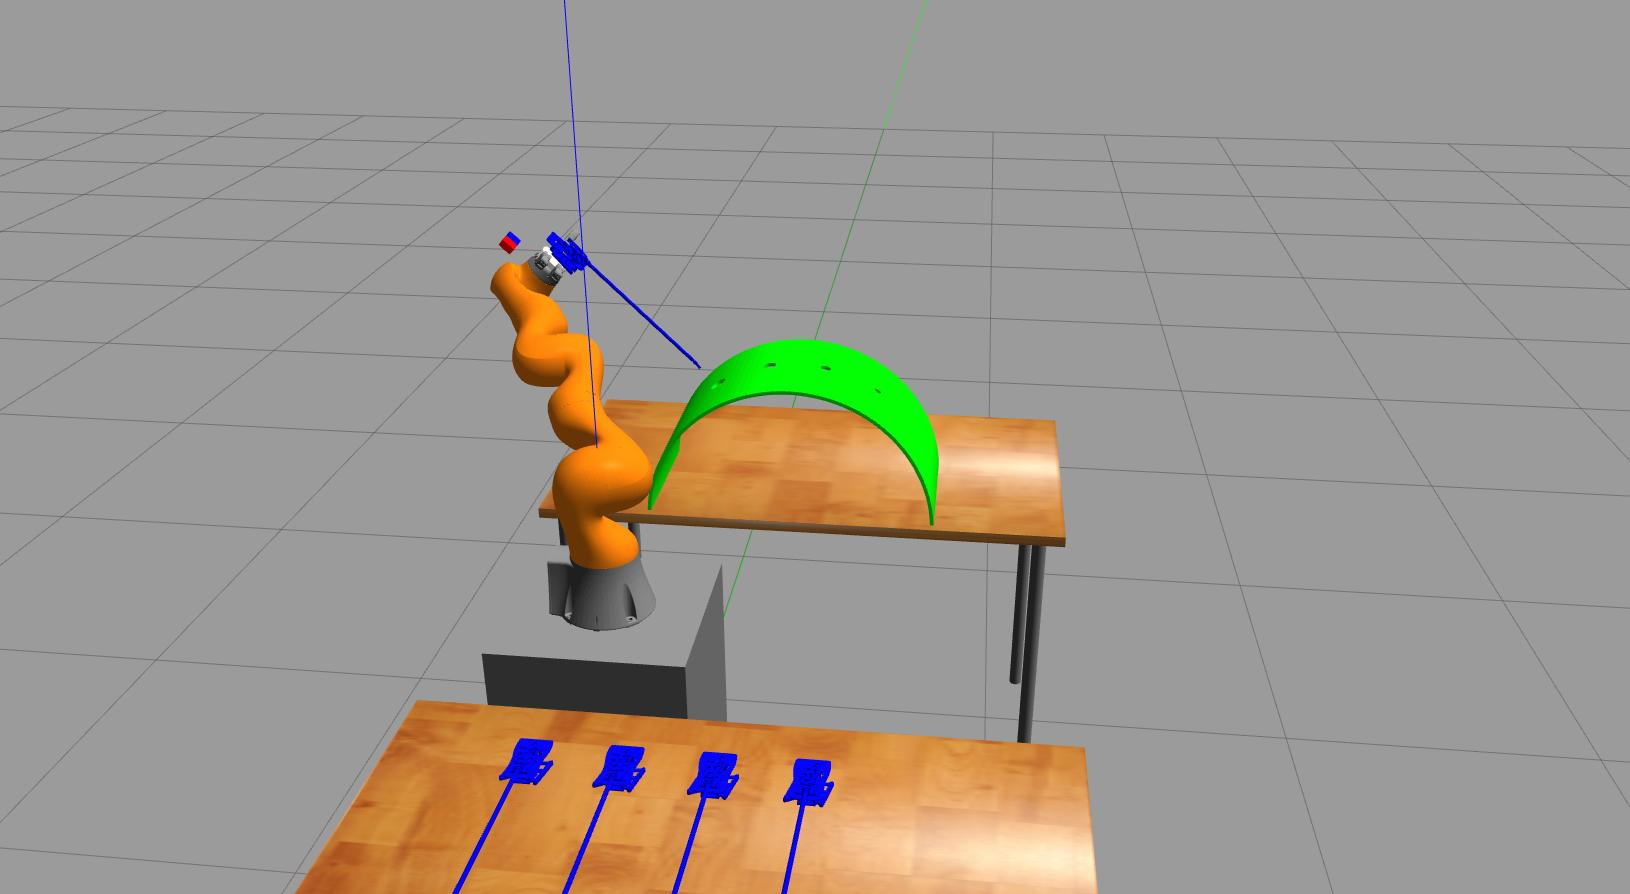
\includegraphics[width=0.31\textwidth]{images/robot_planner2/robot_planner2_2}
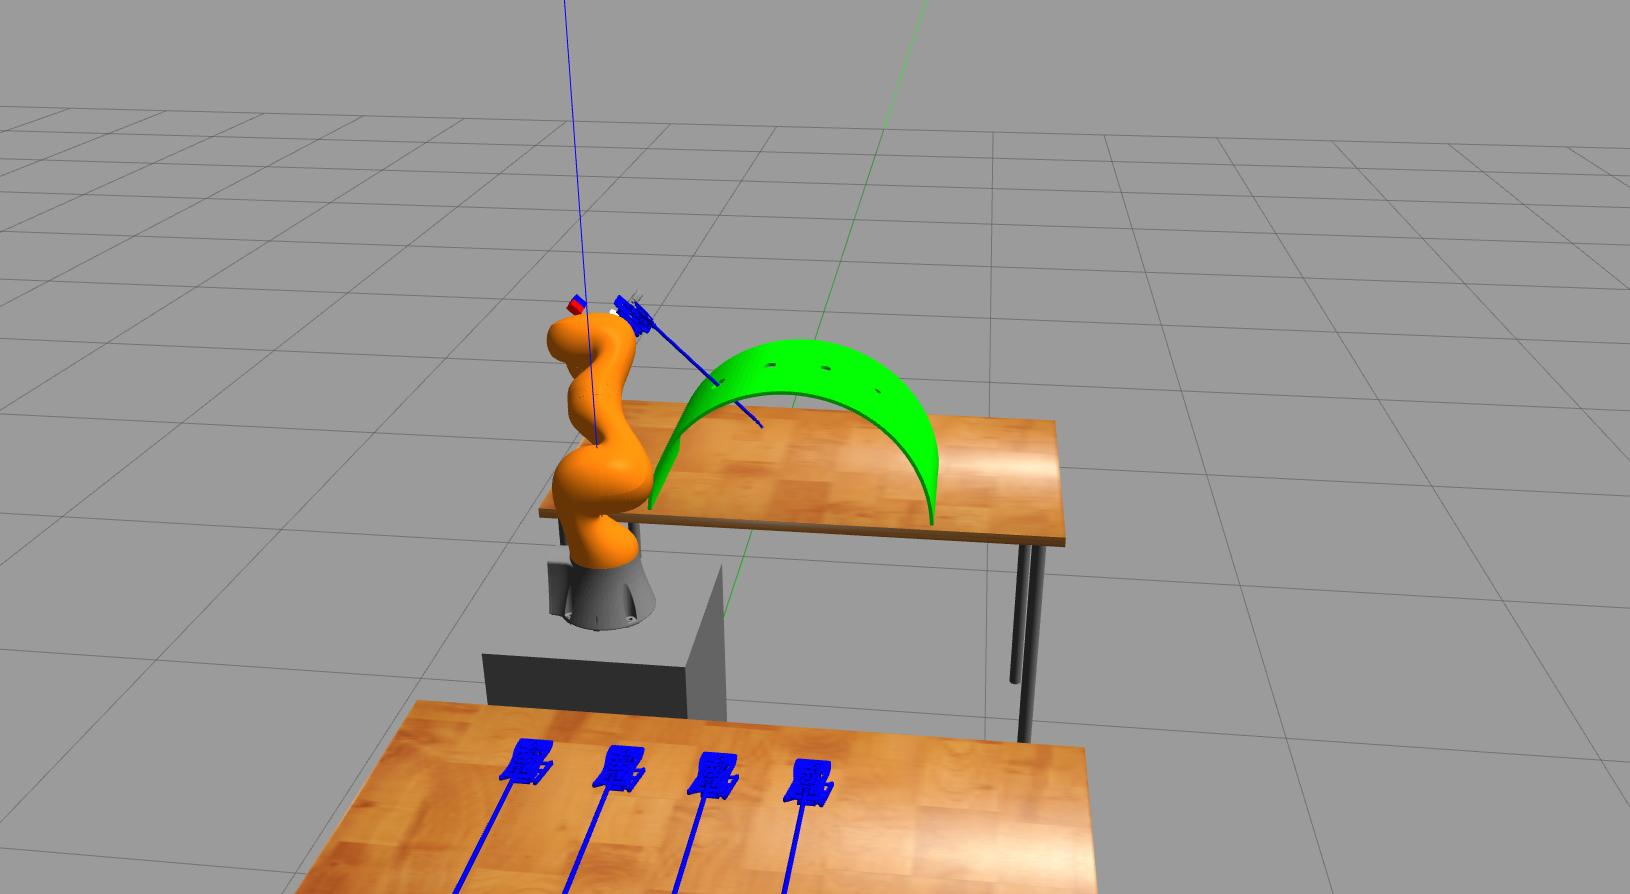
\includegraphics[width=0.31\textwidth]{images/robot_planner2/robot_planner2_3}\\
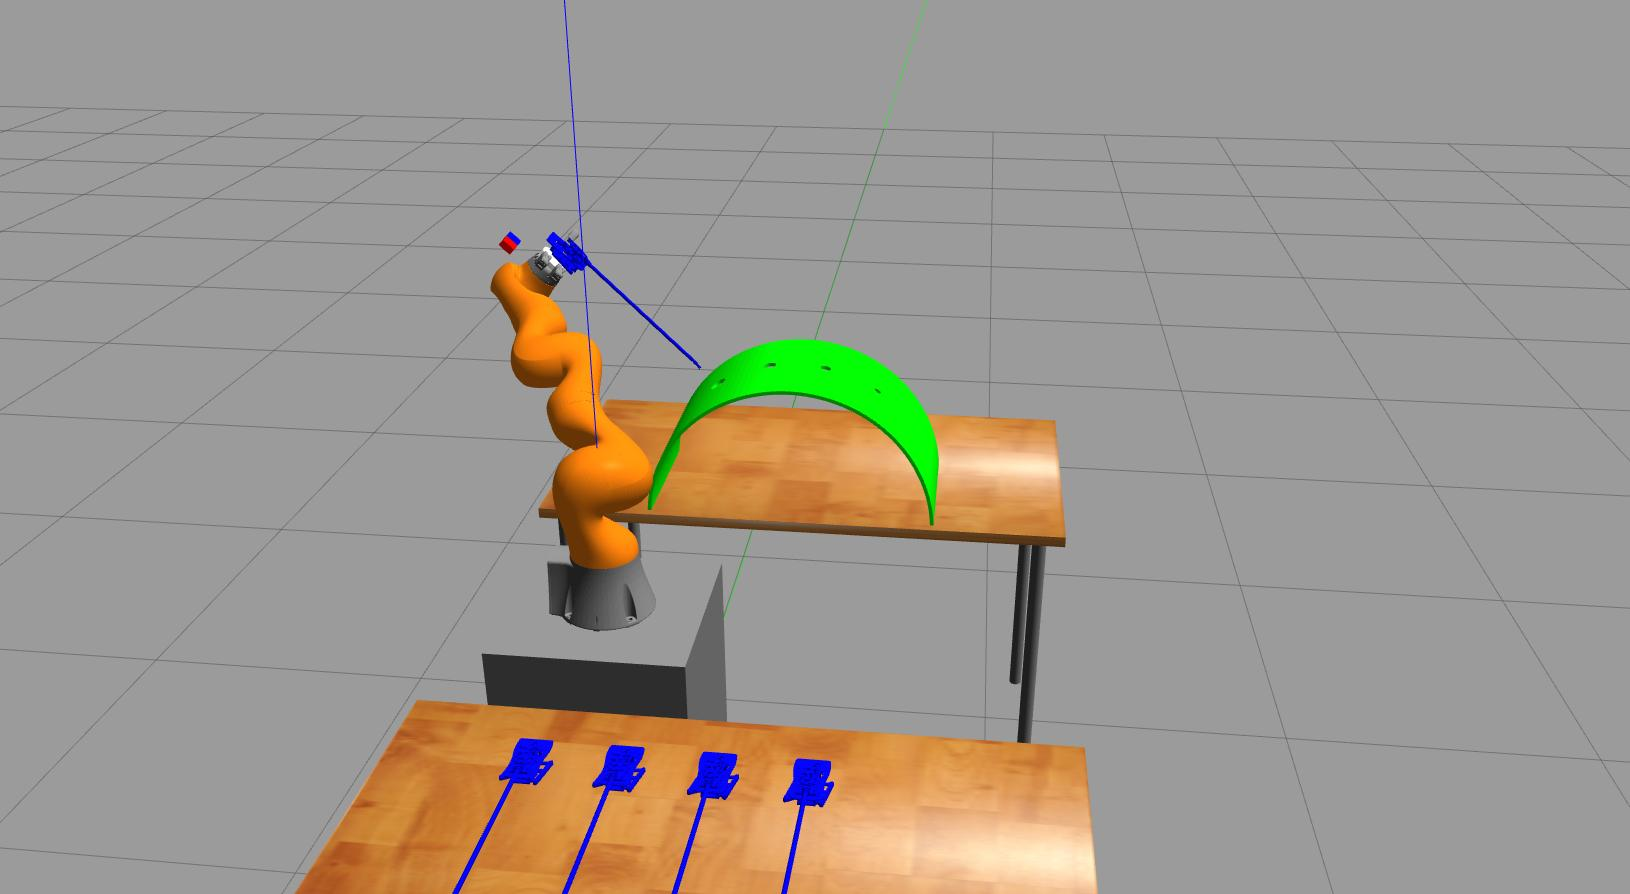
\includegraphics[width=0.31\textwidth]{images/robot_planner2/robot_planner2_4}
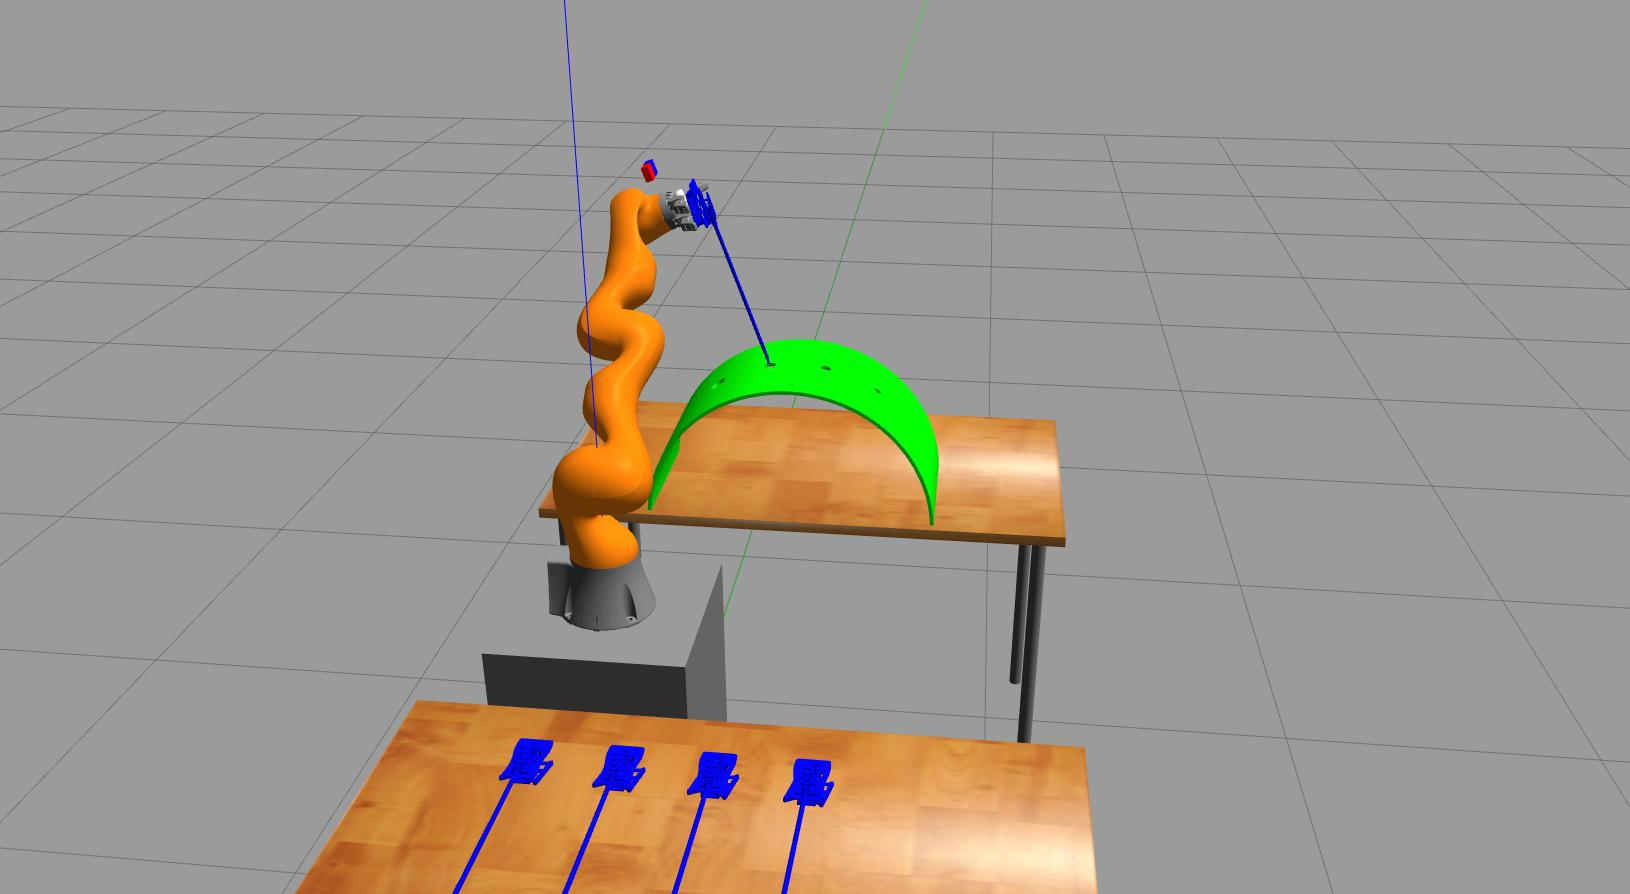
\includegraphics[width=0.31\textwidth]{images/robot_planner2/robot_planner2_5}
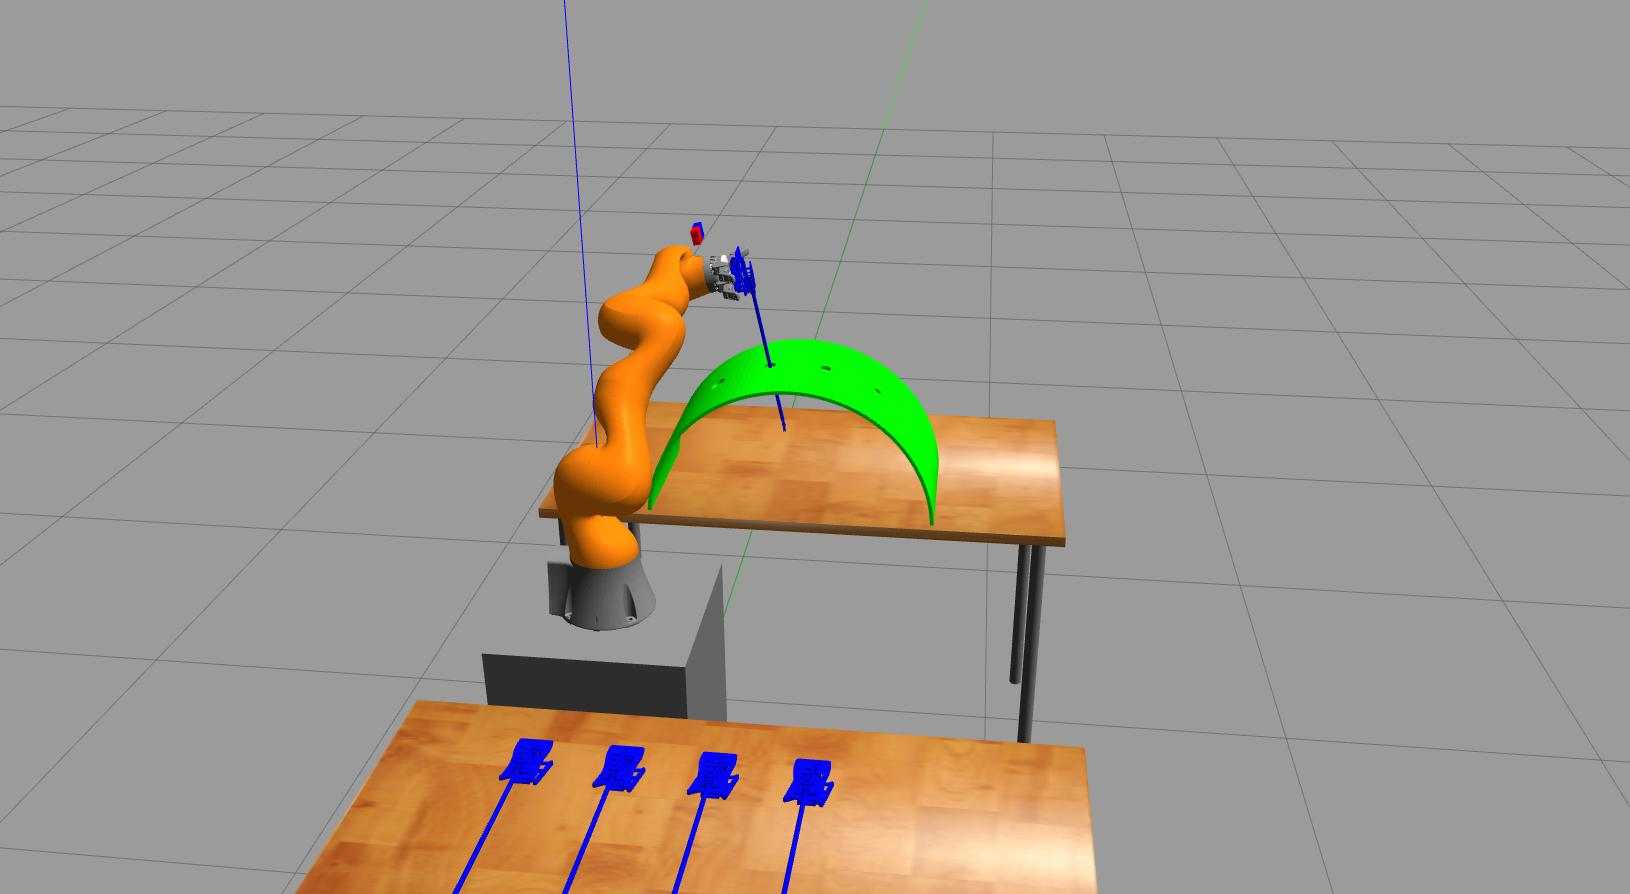
\includegraphics[width=0.31\textwidth]{images/robot_planner2/robot_planner2_6}\\
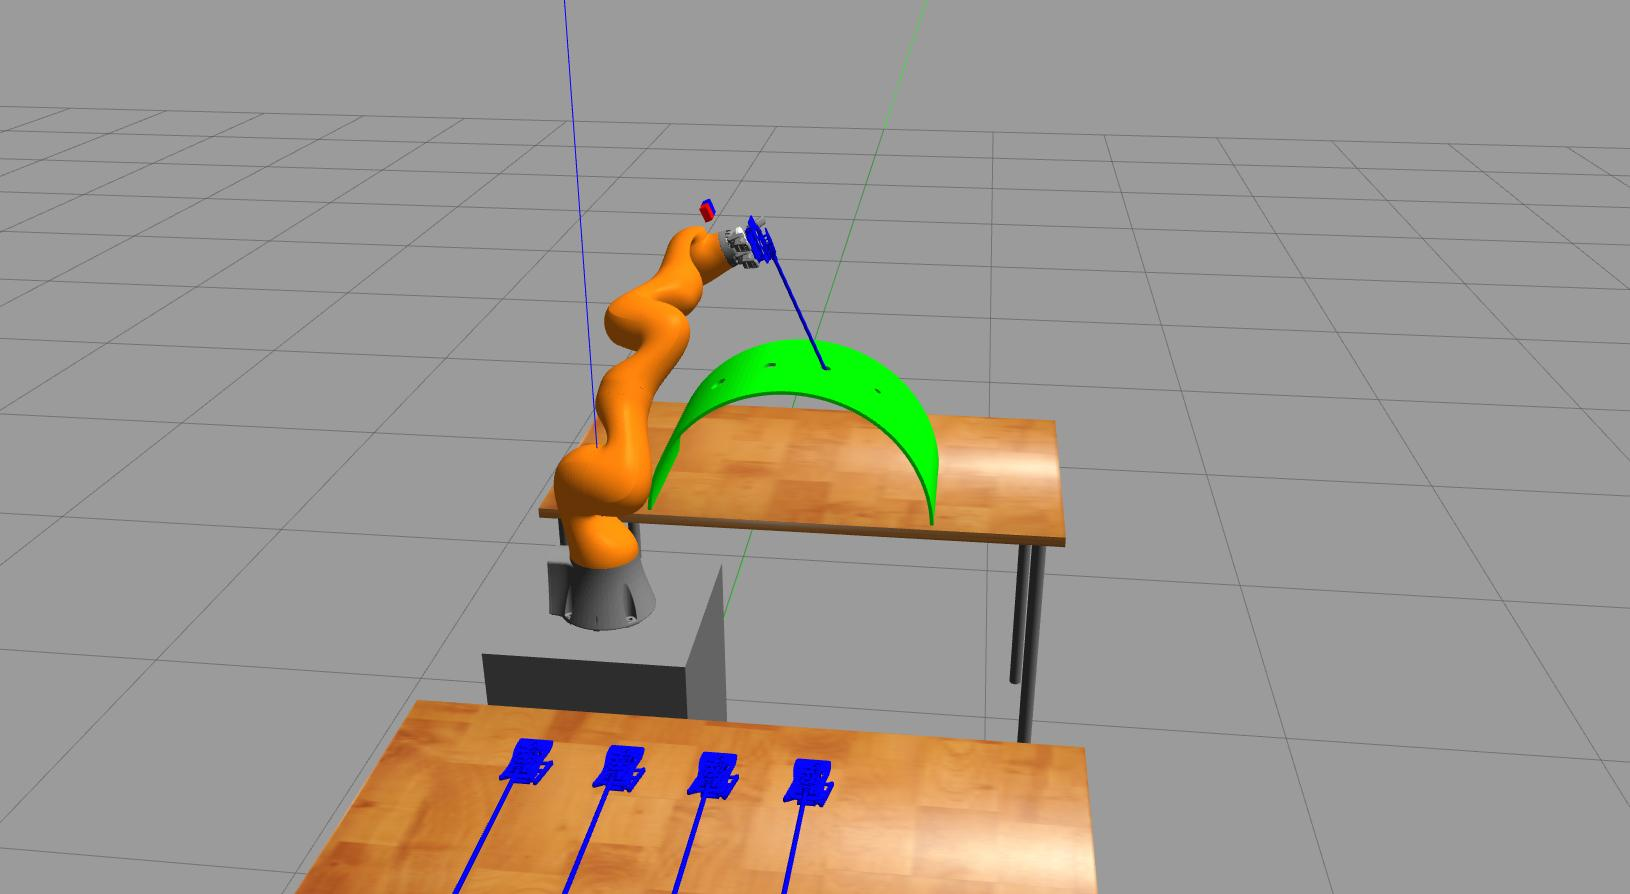
\includegraphics[width=0.31\textwidth]{images/robot_planner2/robot_planner2_7}
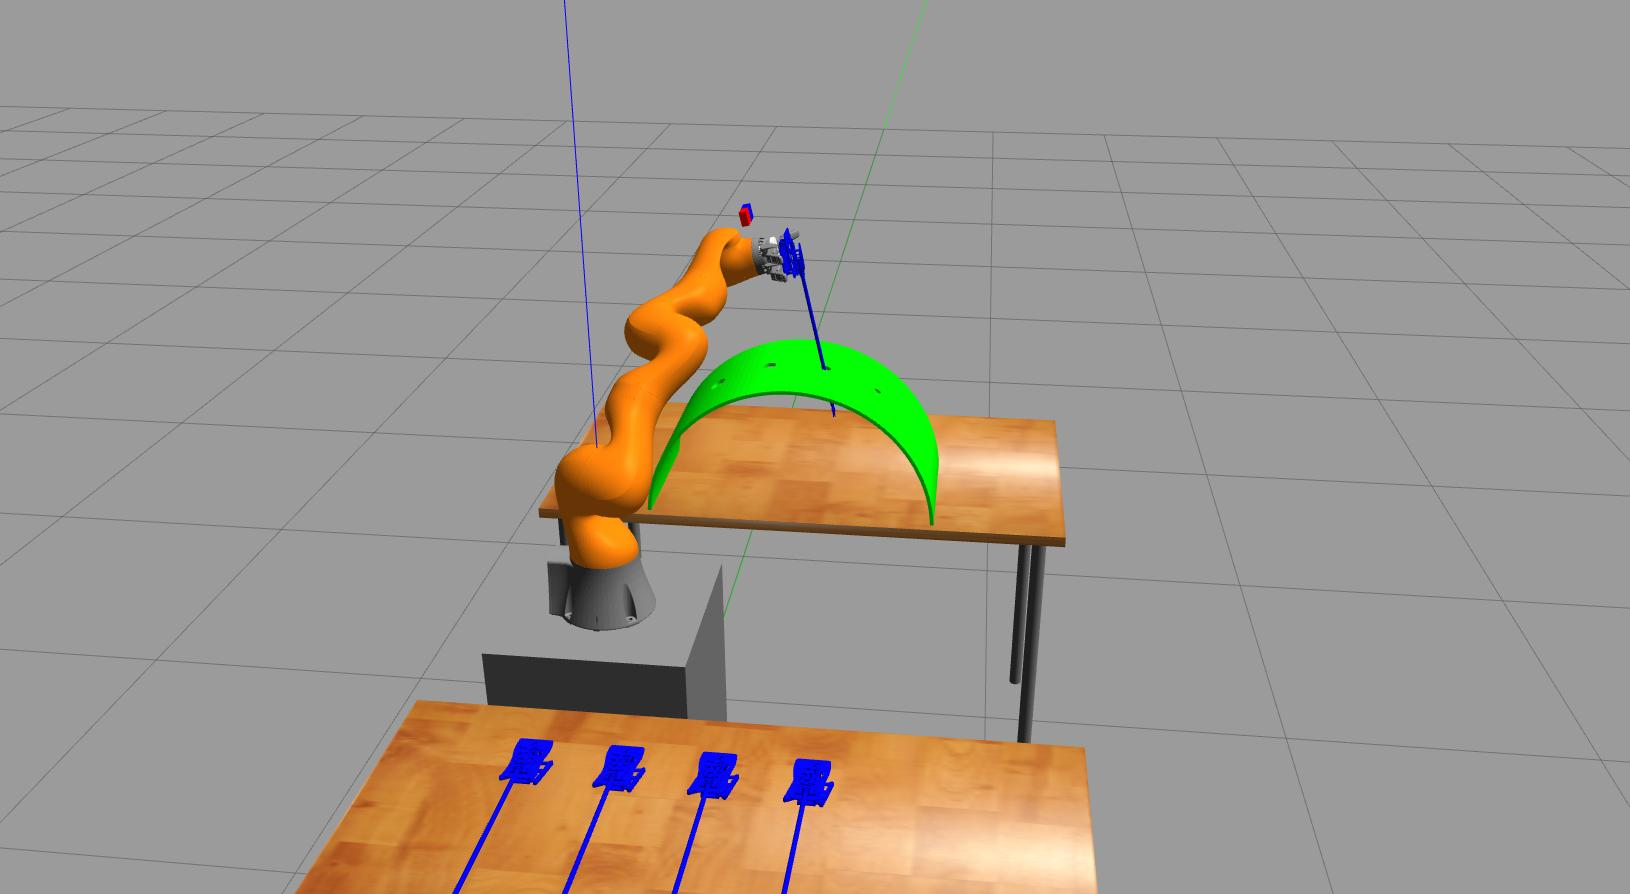
\includegraphics[width=0.31\textwidth]{images/robot_planner2/robot_planner2_8}\\
\caption{Experiment 2a:}
\label{experiment-robot-planner2a}
\end{figure}
\end{center}

% Robot Planner 2a with RRTConnect
\begin{longtable}{|p{2cm}|c|p{2cm}|p{2cm}|p{2cm}|}
\hline
Robot Planner 2a           & \multicolumn{4}{c}{\textbf{RRTConnect}}                                                                                                 \vline \\
\hline
                          & \multicolumn{4}{c}{\textbf{Insertion \& Pivot trajectories}}                     \vline \\
\hline
Experiment                & Trocar1 insertion time & Execution status & Trocar1 reverse insertion time & Execution status  \\
\hline
1	& 0.060728	& 1	& 2.875072	& 1 \\
2	& 0.070508	& 1	& 5.235667	& 1 \\
3	& 0.071487	& 1	& 5.239014	& 1 \\
4	& 0.059288	& 1	& 1.733352	& 1 \\
5	& 0.053619	& 1	& 3.376982	& 1 \\
6	& 0.062	& 1	& 5.389454	& 1 \\
7	& 0.084007	& 1	& -	& 0 \\
8	& 0.058306	& 1	& 5.254352	& 1 \\
9	& 0.046925	& 1	& 4.90185	& 1 \\
10	& 0.060491	& 1	& 5.073171	& 1 \\
\hline
\textbf{Average} & 	0.062736	& 1	& 4.342102	& 0.9 \\
\hline
                          & \multicolumn{4}{c}{\textbf{Insertion \& Pivot trajectories}}                     \vline \\
\hline
Experiment                & Approach trocar2 time & Execution status & Trocar2 insertion time & Execution status  \\
\hline
1 & 2.67618	& 1	& 0.168283	& 1 \\
2 & 5.187283	& 1	& 0.179048	& 1 \\
3 & 0.050117	& 1	& 0.057194	& 1 \\
4 & 1.538822	& 1	& 0.184641	& 1 \\
5 & 1.62114	& 1	& 0.253224	& 1 \\
6 & 5.397757	& 1	& 0.268188	& 1 \\
7 & 5.379305	& 1	& 0.384924	& 1 \\
8 & 5.401832	& 1	& 0.193265	& 1 \\
9 & 2.845741	& 1	& 0.267069	& 1 \\
10  & 5.355111	& 1	& 0.250265	& 1 \\
\hline
\textbf{Average} & 3.545329	& 1	& 0.220610	& 1 \\
\hline
                          & \multicolumn{4}{c}{\textbf{Insertion \& Pivot trajectories}}                     \vline \\
\hline
Experiment                & Trocar2 reverse insertion time & Execution status & Approach trocar3 time & Execution status  \\
\hline
1 & 0.152233	& 1	& 0.214332	& 1 \\
2 & 0.321677	& 1	& 0.361712	& 1 \\
3 & 5.404121	& 1	& 5.271597	& 1 \\
4 & 0.147981	& 1	& 0.15915	& 1 \\
5 & 0.333447	& 1	& 0.298799	& 1 \\
6 & 0.246624	& 1	& 0.209347	& 1 \\
7 & 0.381983	& 1	& 0.473779	& 1 \\
8 & 0.219369	& 1	& 0.167211	& 1 \\
9 & 0.227563	& 1	& 0.297372	& 1 \\
10  & 5.149372	& 1	& 5.3578	& 1 \\
\hline
\textbf{Average} & 1.258437	& 1	& 1.281110	& 1 \\
\hline
                          & \multicolumn{4}{c}{\textbf{Insertion \& Pivot trajectories}}                     \vline \\
\hline
Experiment                & Trocar3 insertion time & Execution status & Trocar3 reverse insertion time & Execution status  \\
\hline
1 & 0.196175	& 1	& 0.855452	& 0 \\
2 & 0.412455	& 1	& 1.133213	& 0 \\
3 & 0.355923	& 1	& 0.814161	& 0 \\
4 & 0.194839	& 1	& 0.885119	& 0 \\
5 & 0.351561	& 1	& 0.364089	& 0 \\
6 & 0.355251	& 1	& 0.826636	& 0 \\
7 & 0.336123	& 1	& 0.30715	& 1 \\
8 & 0.147867	& 1	& 1.053035	& 0 \\
9 & 0.347956	& 0.6	& 0.80884	& 0.37  \\
10  & 0.28364	& 0.6	& 0.229825	& 1 \\
\hline
\textbf{Average} & 	0.298179	& 0.92 &	0.727752	& 0.237 \\
\hline

\caption{Time results for robot planner 2a using the RRTConnect path planner algorithm. Planning time is the sum of solution time and path simplification time. Execution status is 
1 for success and 0 for failure. Parameters: tolerances: 0.0005, max planning time: 5 seconds, replanning: true, max planning attempts: 6. Experiments start from home position.}
\label{robot-planner2a-rrtconnect-data}
\end{longtable}

To overcome the reachability issue shown in Figure \ref{experiment-robot-planner2a}, the algorithm was repeated, but this time using a different simulation layout 
in Gazebo, in which the mounting dock is closer to the robot and in front of it. This new layout enables the robot to reach all mounting holes with ease and 
with sufficient dexterity, the robot is free to pivot around.

\begin{center}
\begin{figure}[H]
\centering
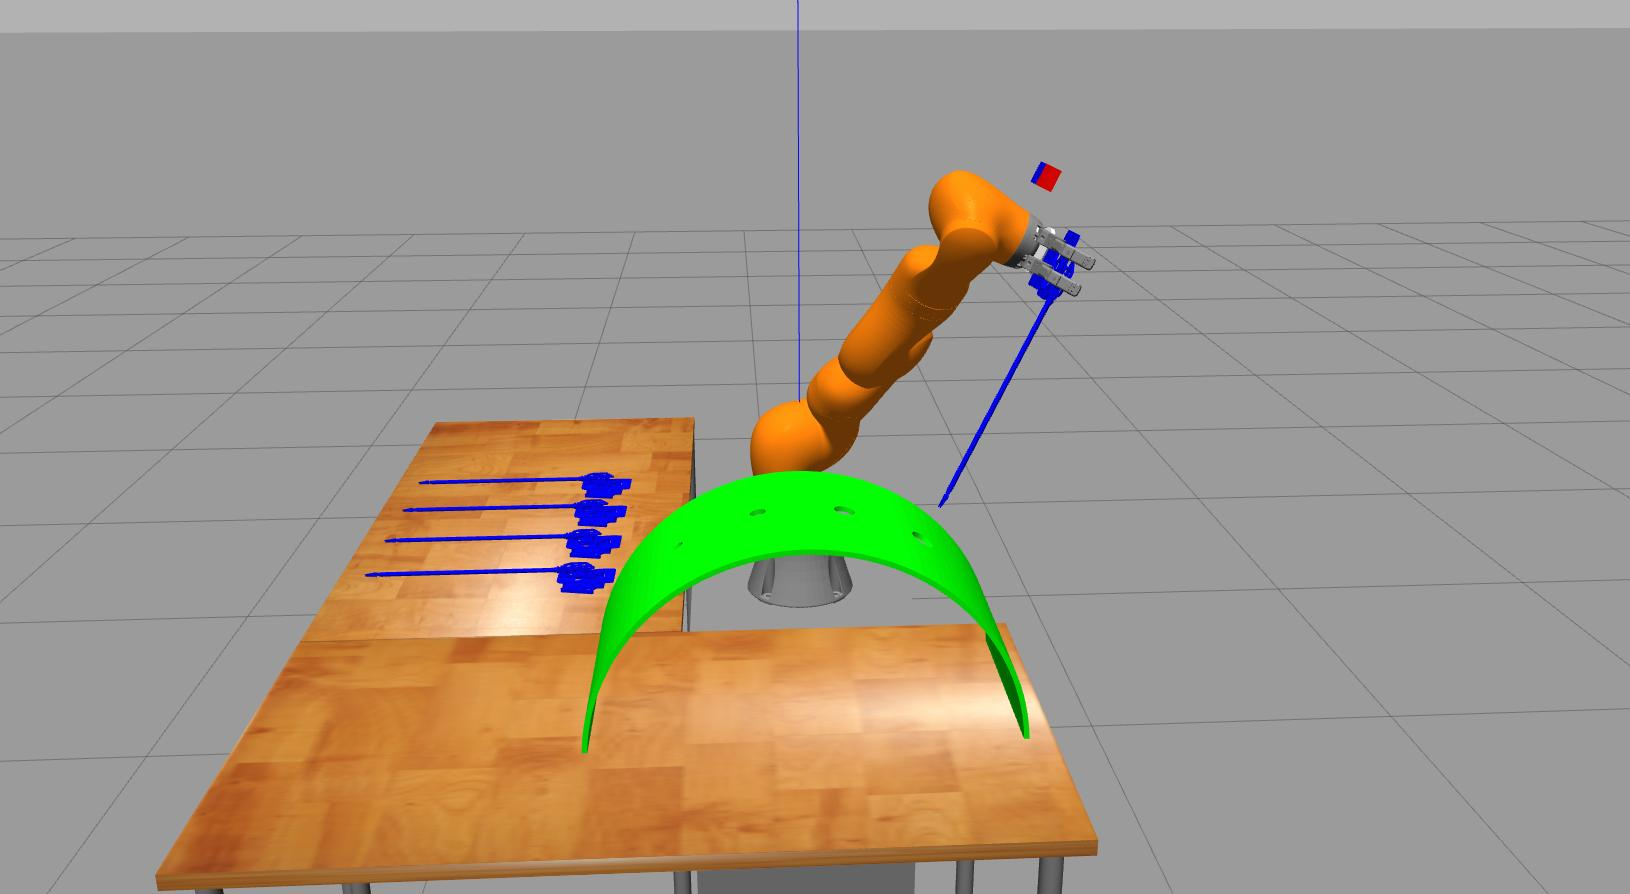
\includegraphics[width=0.3\textwidth]{images/robot_planner2b/robot_planner2b_1}
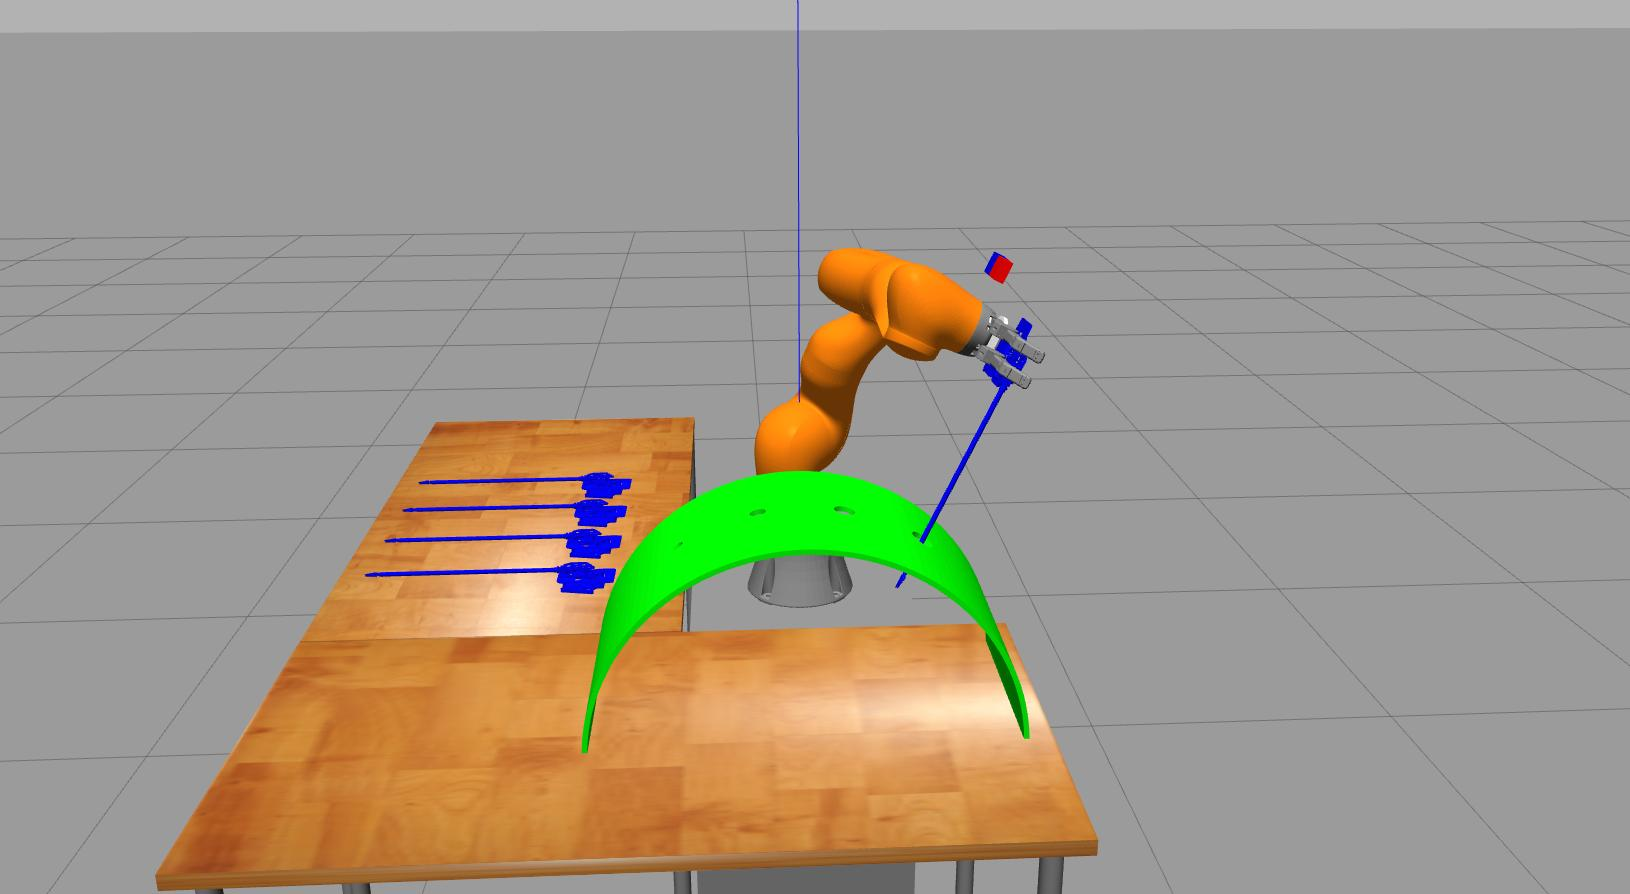
\includegraphics[width=0.3\textwidth]{images/robot_planner2b/robot_planner2b_2}
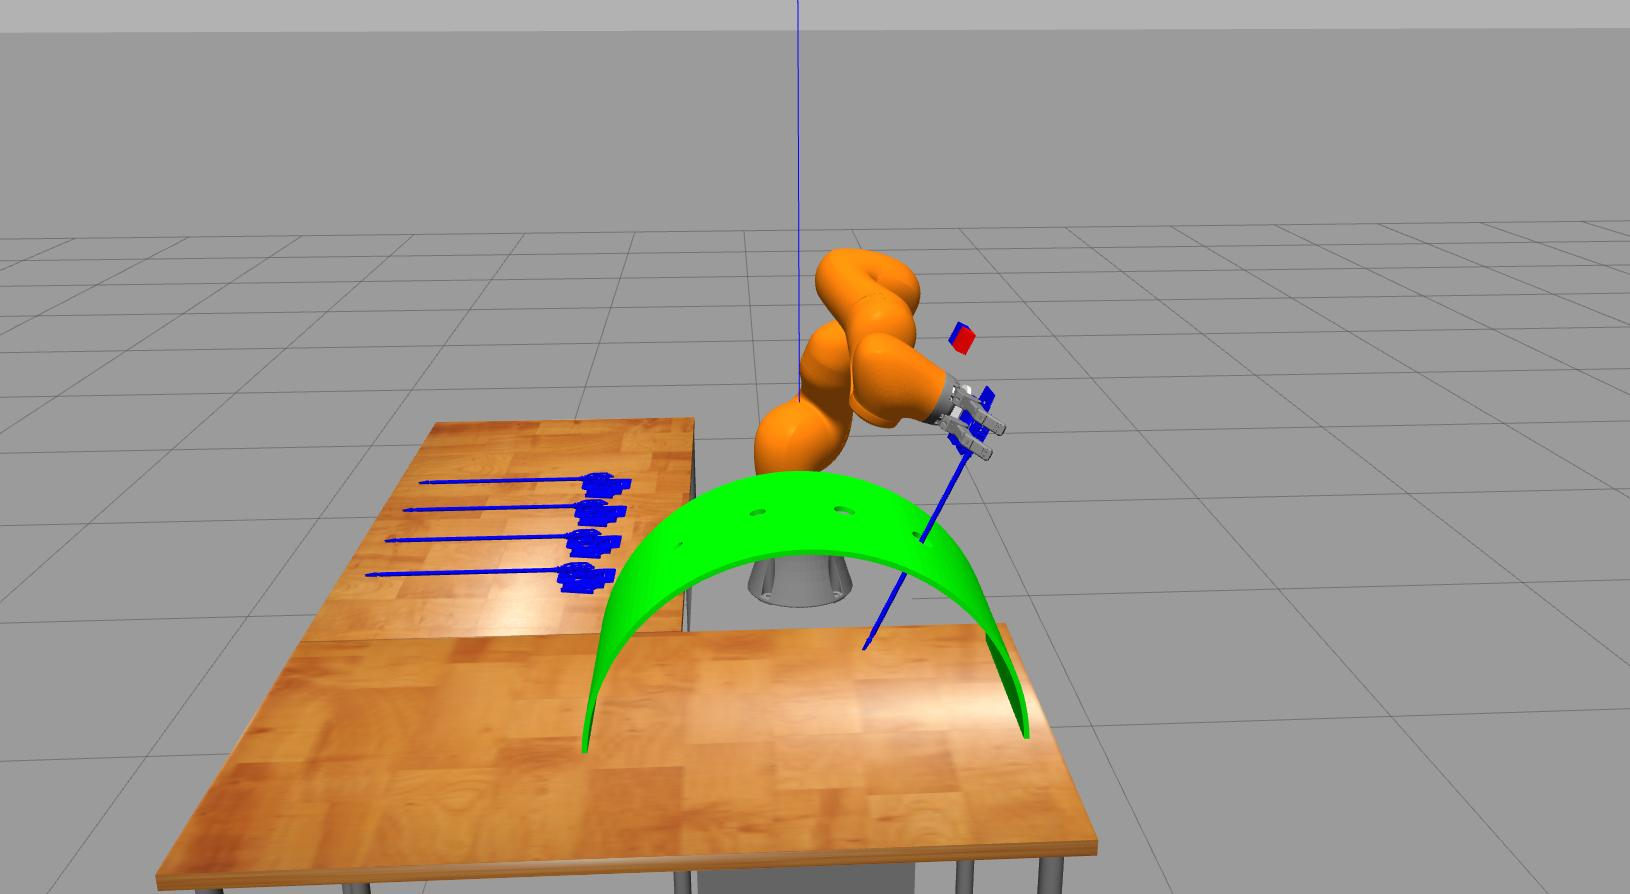
\includegraphics[width=0.3\textwidth]{images/robot_planner2b/robot_planner2b_3}\\
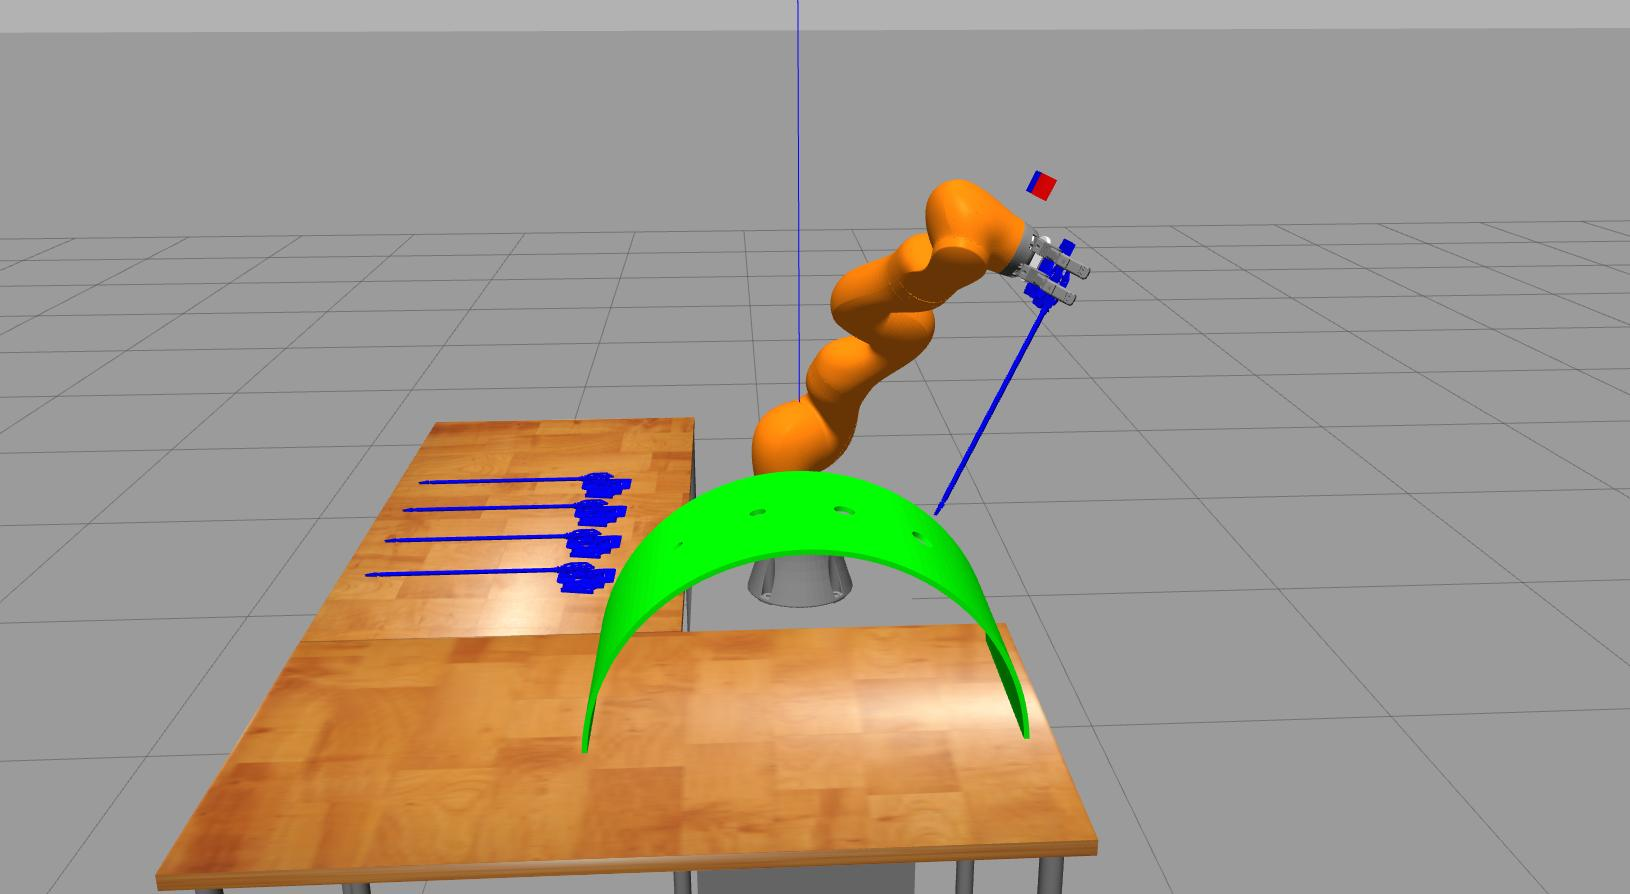
\includegraphics[width=0.3\textwidth]{images/robot_planner2b/robot_planner2b_4}
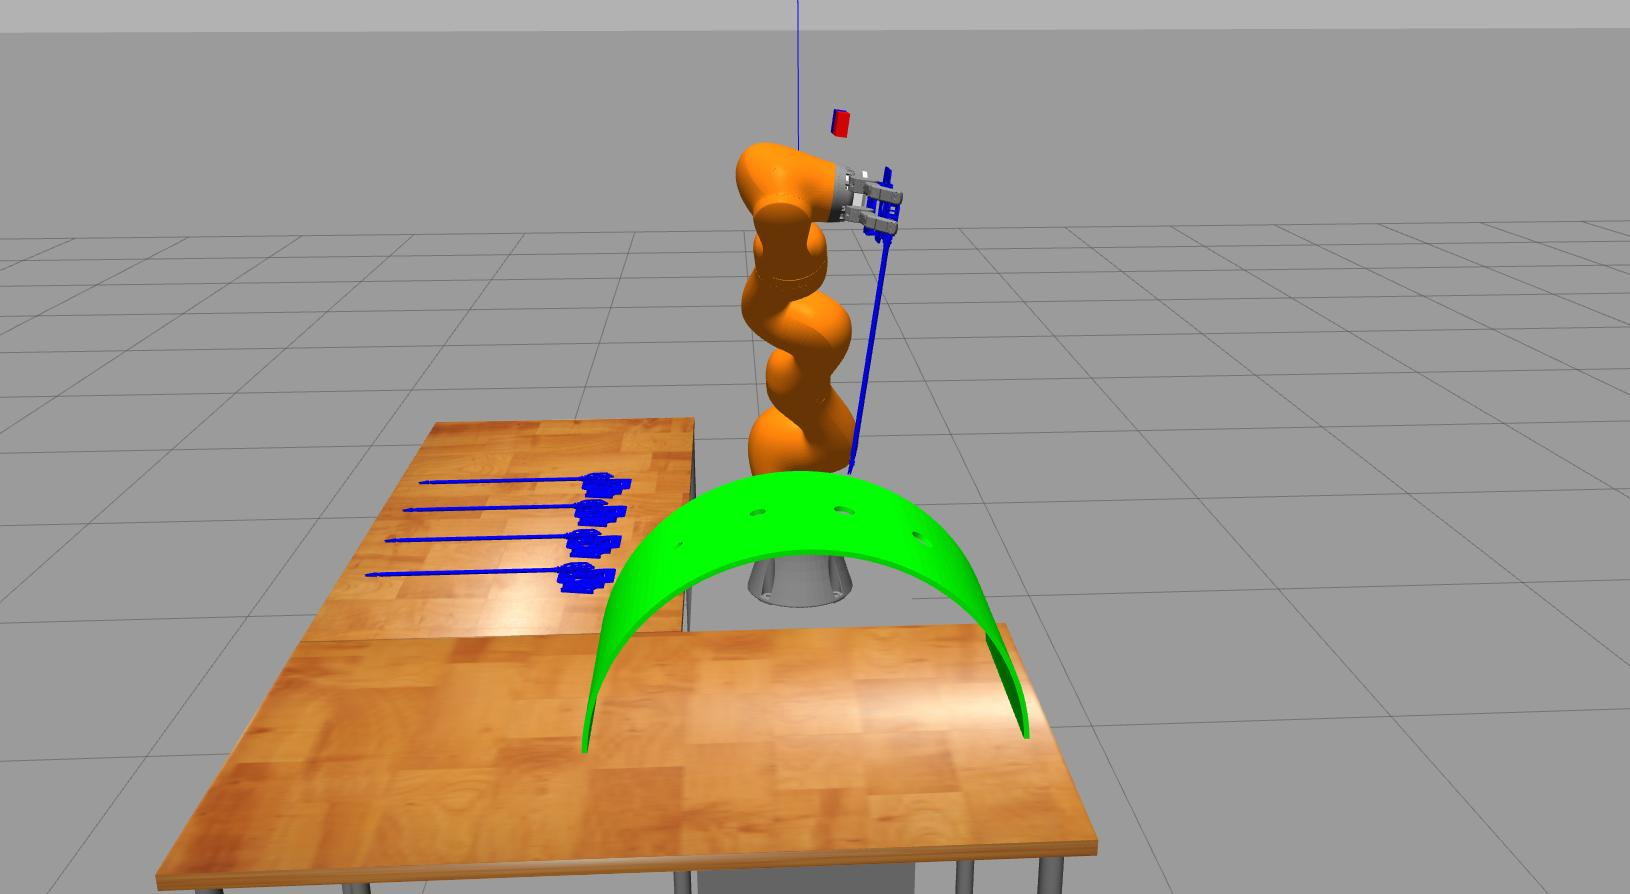
\includegraphics[width=0.3\textwidth]{images/robot_planner2b/robot_planner2b_5}
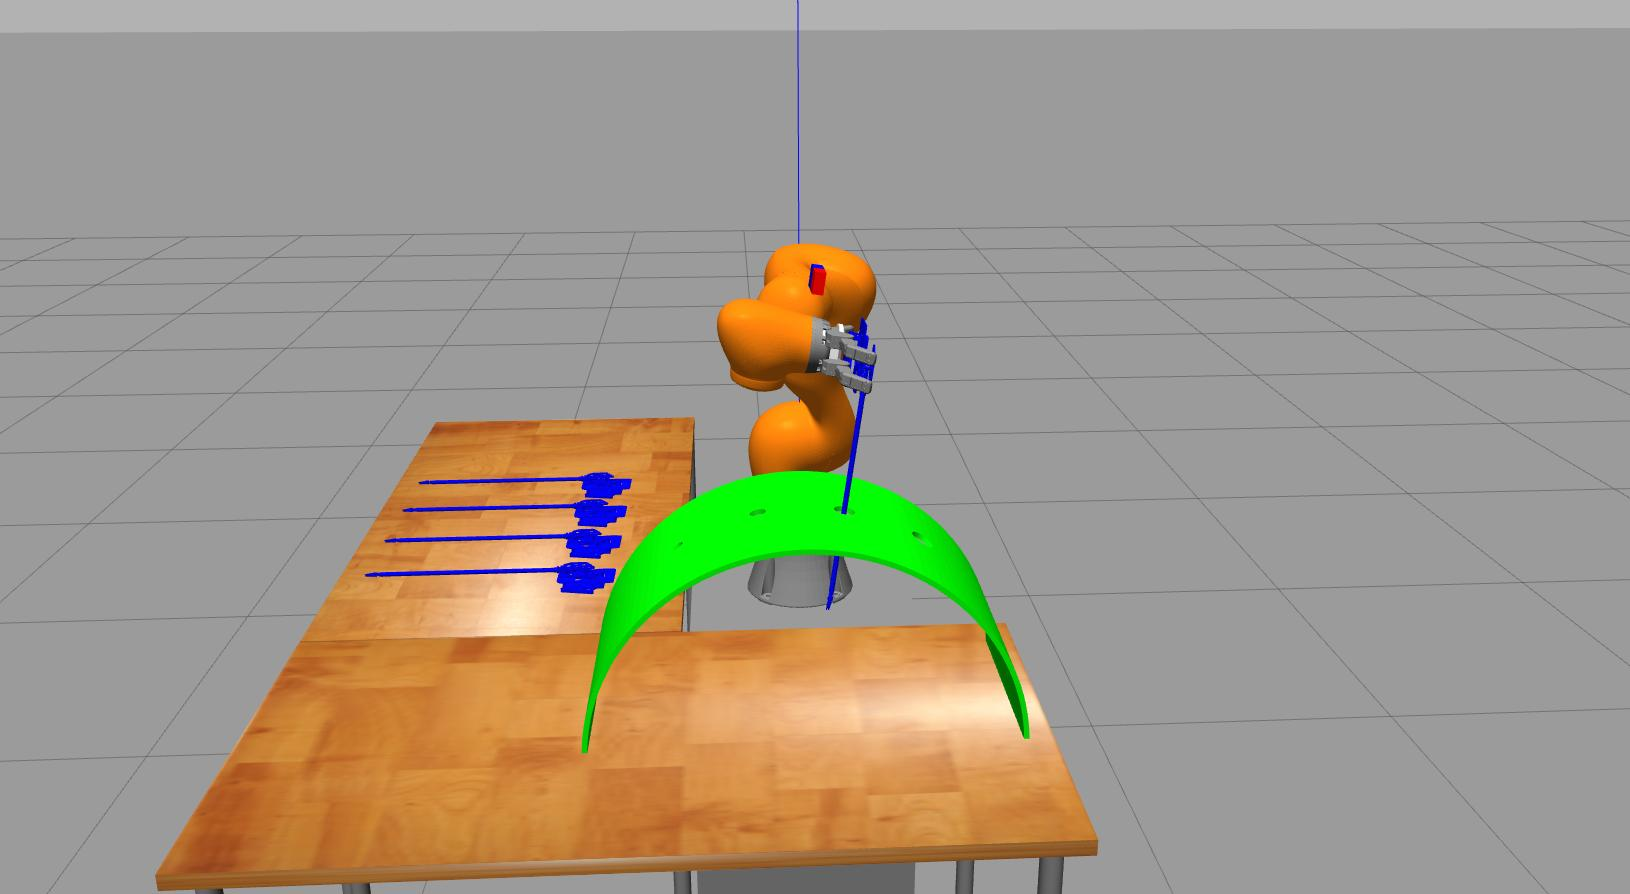
\includegraphics[width=0.3\textwidth]{images/robot_planner2b/robot_planner2b_6}\\
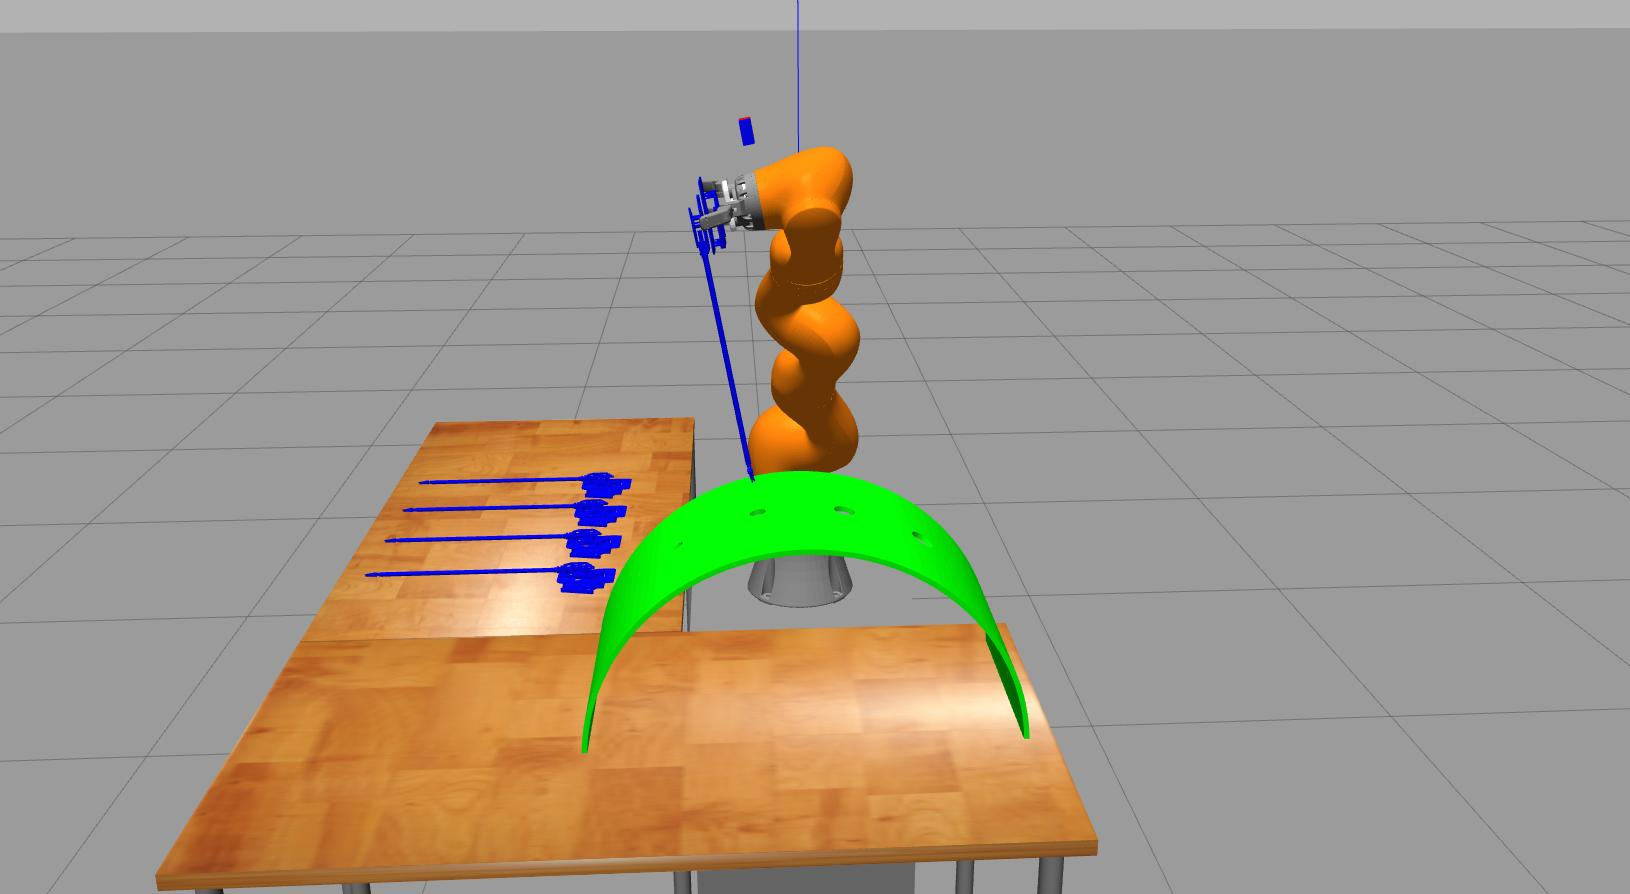
\includegraphics[width=0.3\textwidth]{images/robot_planner2b/robot_planner2b_7}
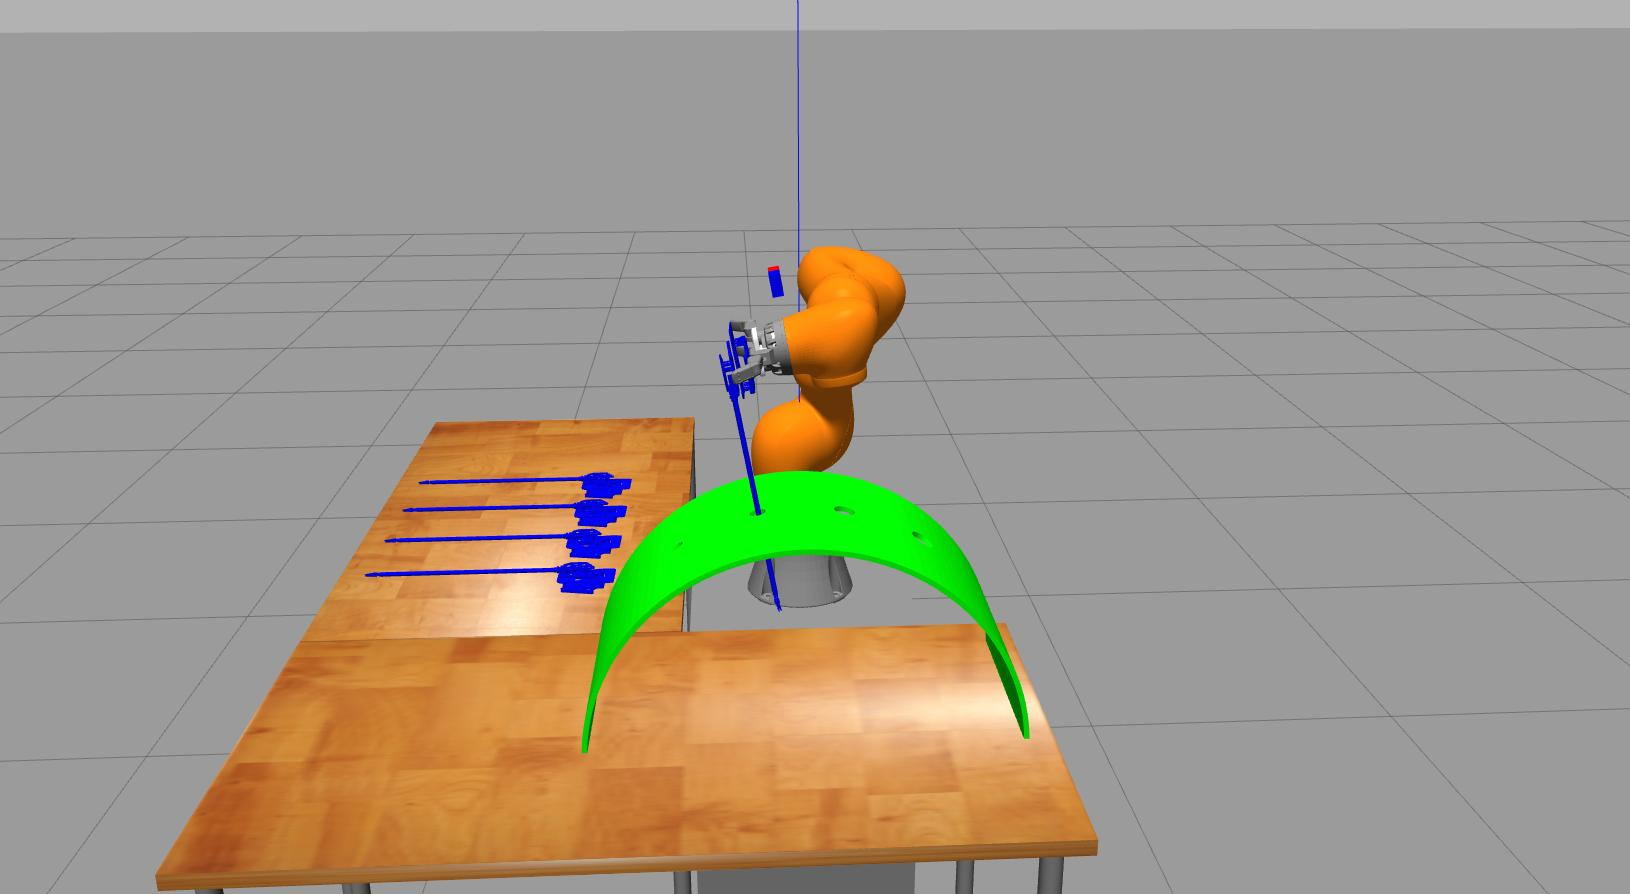
\includegraphics[width=0.3\textwidth]{images/robot_planner2b/robot_planner2b_8}
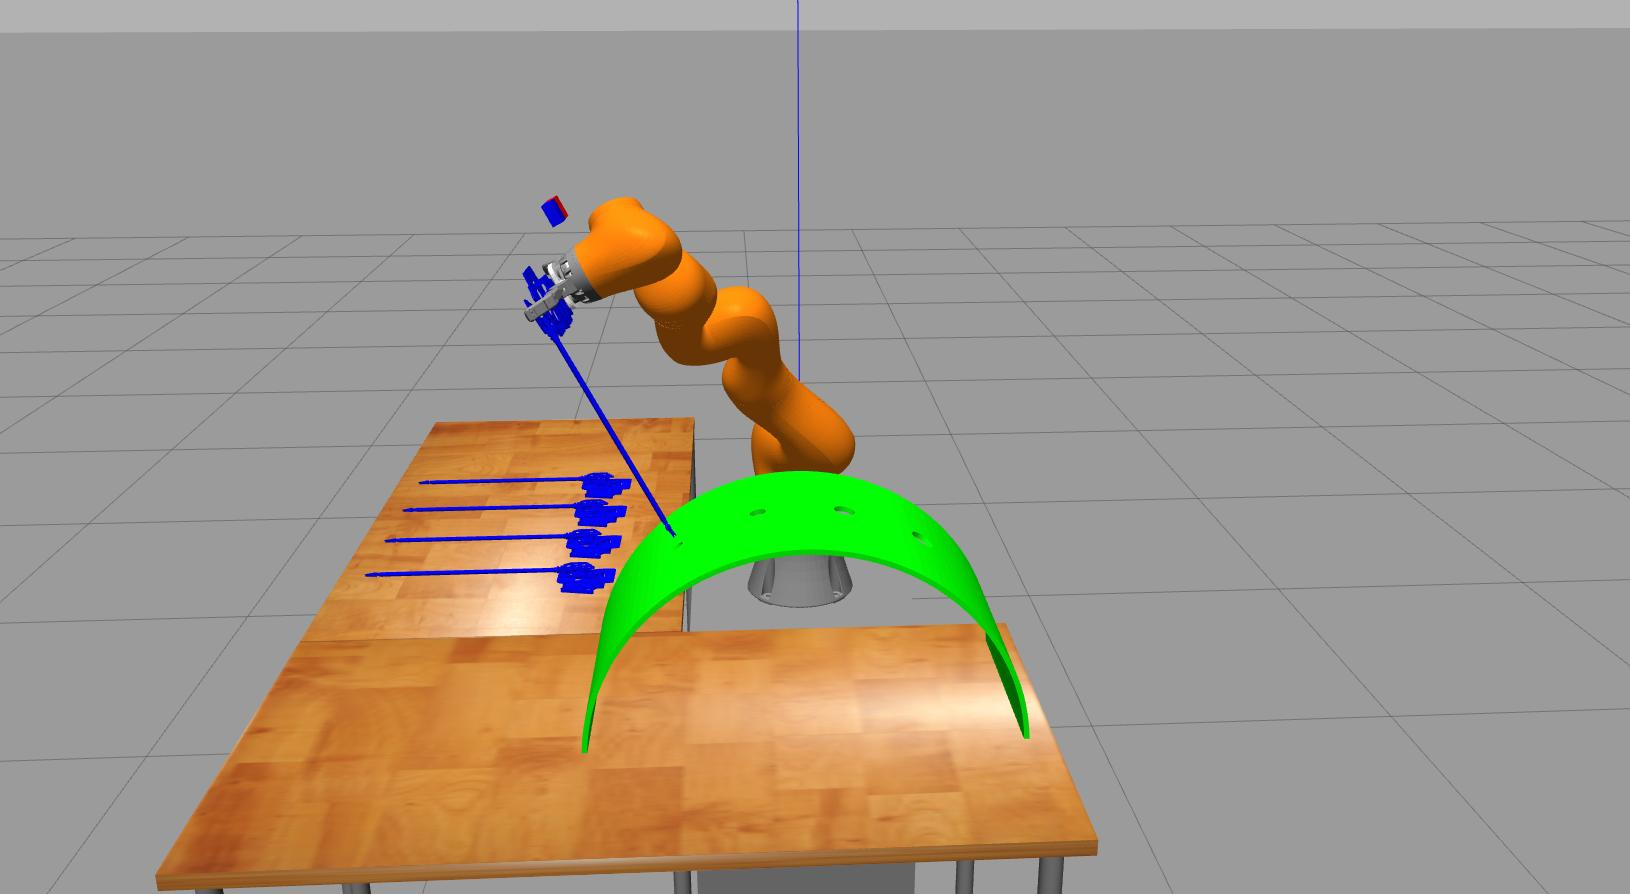
\includegraphics[width=0.3\textwidth]{images/robot_planner2b/robot_planner2b_9}\\
\caption{Experiment 2b: Running robot planner 2b with a different table layout so that all target poses have improved reachability. Note that all trajectories shown in the screenshots are collision-free, 
because the robotic arm is in an elbow-up configuration, so that it avoids the collision between the 3rd link of the robot and the mounting dock (green object shown in simulation).}
\label{experiment-robot-planner2b}
\end{figure}
\end{center}

Observing the screenshots at figure \ref{experiment-robot-planner2b}, it is clear that the robot must always be in an elbow-up configuration in order to avoid collisions with the mounting dock. This constraint can be 
described either using the relative distance of the third link with the base or the relative angles of the third link's axis with respect to the axis of the base, as described with more detail in 
\ref{section-elbow-up-constraints}. The latter description with angles is easier to implement using the ROS MoveIt! framework,  but it would require to solve an extra inverse and forward kinematics problem targeting the third 
link, instead of the end-effector. To avoid these additional, computationally expensive calculations and simplify the experiments, instead of mathematically describing the constraint, 
some extra points were added in the trajectory. 
These points are usually close to the robot's axis and are such, that 
moveit will be forced to find a solution with an elbow-up configuration (because there will be no other solution satisfying the target point). Starting with an elbow-up configuration makes the path planner stick with that 
configuration for most of the path, because otherwise it would make a big jump in the joint state space which is not allowed from the parameters used in the experiments.

% Robot Planner 2b with RRTConnect
\begin{longtable}{|p{2cm}|c|p{2cm}|p{2cm}|p{2cm}|}
\hline
Robot Planner 2b           & \multicolumn{4}{c}{\textbf{RRTConnect}}                                                                                                 \vline \\
\hline
                          & \multicolumn{4}{c}{\textbf{Insertion \& Pivot trajectories}}                     \vline \\
\hline
Experiment                & Trocar1 insertion time & Execution status & Trocar1 reverse insertion time & Execution status  \\
\hline
1	& 0.269901	& 1	& 0.355588	& 1 \\
2	& 0.220509	& 1	& 0.255968	& 1 \\
3	& 0.260483	& 1	& 5.28604	& 1 \\
4	& 0.267778	& 1	& 0.267796	& 1 \\
5	& 0.388487	& 1	& 5.321684	& 1 \\
6	& 0.316275	& 1	& 0.2088	& 1 \\
7	& 0.202614	& 1	& 0.14469	& 1 \\
8	& 0.289368	& 1	& 0.275917	& 1 \\
9	& 0.353631	& 1	& 0.353631	& 1 \\
10	& 0.185345	& 1	& 0.154755	& 1 \\
\hline
\textbf{Average} & 0.275439 &	1	& 1.262487	& 1 \\
\hline
                          & \multicolumn{4}{c}{\textbf{Insertion \& Pivot trajectories}}                     \vline \\
\hline
Experiment                & Approach trocar2 time & Execution status & Trocar2 insertion time & Execution status  \\
\hline
1 & 0.322578	& 1	& 0.283497	& 1 \\
2 & 0.209871	& 1	& 0.410543	& 1 \\
3 & 5.099769	& 1	& 0.296228	& 1 \\
4 & 0.216997	& 1	& 0.342776	& 1 \\
5 & 5.328204	& 1	& 0.394472	& 1 \\
6 & 0.450936	& 1	& 0.249248	& 1 \\
7 & 0.336209	& 1	& 0.165375	& 1 \\
8 & 0.397699	& 1	& 0.202118	& 1 \\
9 & 0.235555	& 1	& 0.333129	& 1 \\
10  & 0.320059	& 1	& 0.343595	& 1 \\
\hline
\textbf{Average} & 1.291788	& 1	& 0.302098	& 1 \\
\hline
                          & \multicolumn{4}{c}{\textbf{Insertion \& Pivot trajectories}}                     \vline \\
\hline
Experiment                & Trocar2 reverse insertion time & Execution status & Approach trocar3 time & Execution status  \\
\hline
1 & 5.374646	& 1	& 5.451335	& 1 \\
2 & 0.452231	& 1	& 0.253669	& 1 \\
3 & 0.22638	& 1	& 0.383933	& 1 \\
4 & 5.371822	& 1	& 5.611649	& 1 \\
5 & 0.395787	& 1	& 0.309212	& 1 \\
6 & 5.15406	& 1	& 5.515007	& 1 \\
7 & 4.189377	& 1	& 5.570568	& 1 \\
8 & 5.167346	& 1	& 5.522056	& 1 \\
9 & 5.101735	& 1	& 5.452301	& 1 \\
10  & 5.273342	& 1	& 5.467273	& 1 \\
\hline
\textbf{Average} & 3.670673	& 1	& 3.953700	& 1 \\
\hline
                          & \multicolumn{4}{c}{\textbf{Insertion \& Pivot trajectories}}                     \vline \\
\hline
Experiment                & Trocar3 insertion time & Execution status & Trocar3 reverse insertion time & Execution status  \\
\hline
1 & 0.372382	& 1	& 5.34059	& 1 \\
2 & 0.280432	& 1	& 0.261765	& 1 \\
3 & 0.179581	& 1	& 0.187589	& 1 \\
4 & 0.121094	& 1	& 5.152808	& 1 \\
5 & 0.472468	& 1	& -	& 0 \\
6 & 0.251195	& 1	& 0.442282	& 0 \\
7 & 0.20647	& 1	& 0.318481	& 1 \\
8 & 0.178941	& 1	& 0.185758	& 1 \\
9 & 0.188906	& 1	& 0.222821	& 1 \\
10  & 0.165681	& 1	& 0.170876	& 1 \\
\hline
\textbf{Average} & 	0.241715  &	1 &	1.364774 &	0.8 \\
\hline
\caption{Time results for robot planner 2b using the RRTConnect path planner algorithm and a different table layout from robot planner 2a. Planning time is the sum of solution time and path simplification time. Execution status is 
1 for success and 0 for failure. Parameters: tolerances: 0.0005, max planning time: 5 seconds, replanning: true, max planning attempts: 6. Experiments start from home position.}
\label{robot-planner2b-rrtconnect-data}
\end{longtable}


Due to the probabilistic nature of the motion planner (in these experiments the OMPL library is used with the RRTConnect path planning algorithm), the solutions 
to the path planning problem are not always the same and thus it is possible that the robot arm reaches a pose which is close to a singularity
\begin{center}
\begin{figure}[H]
\centering
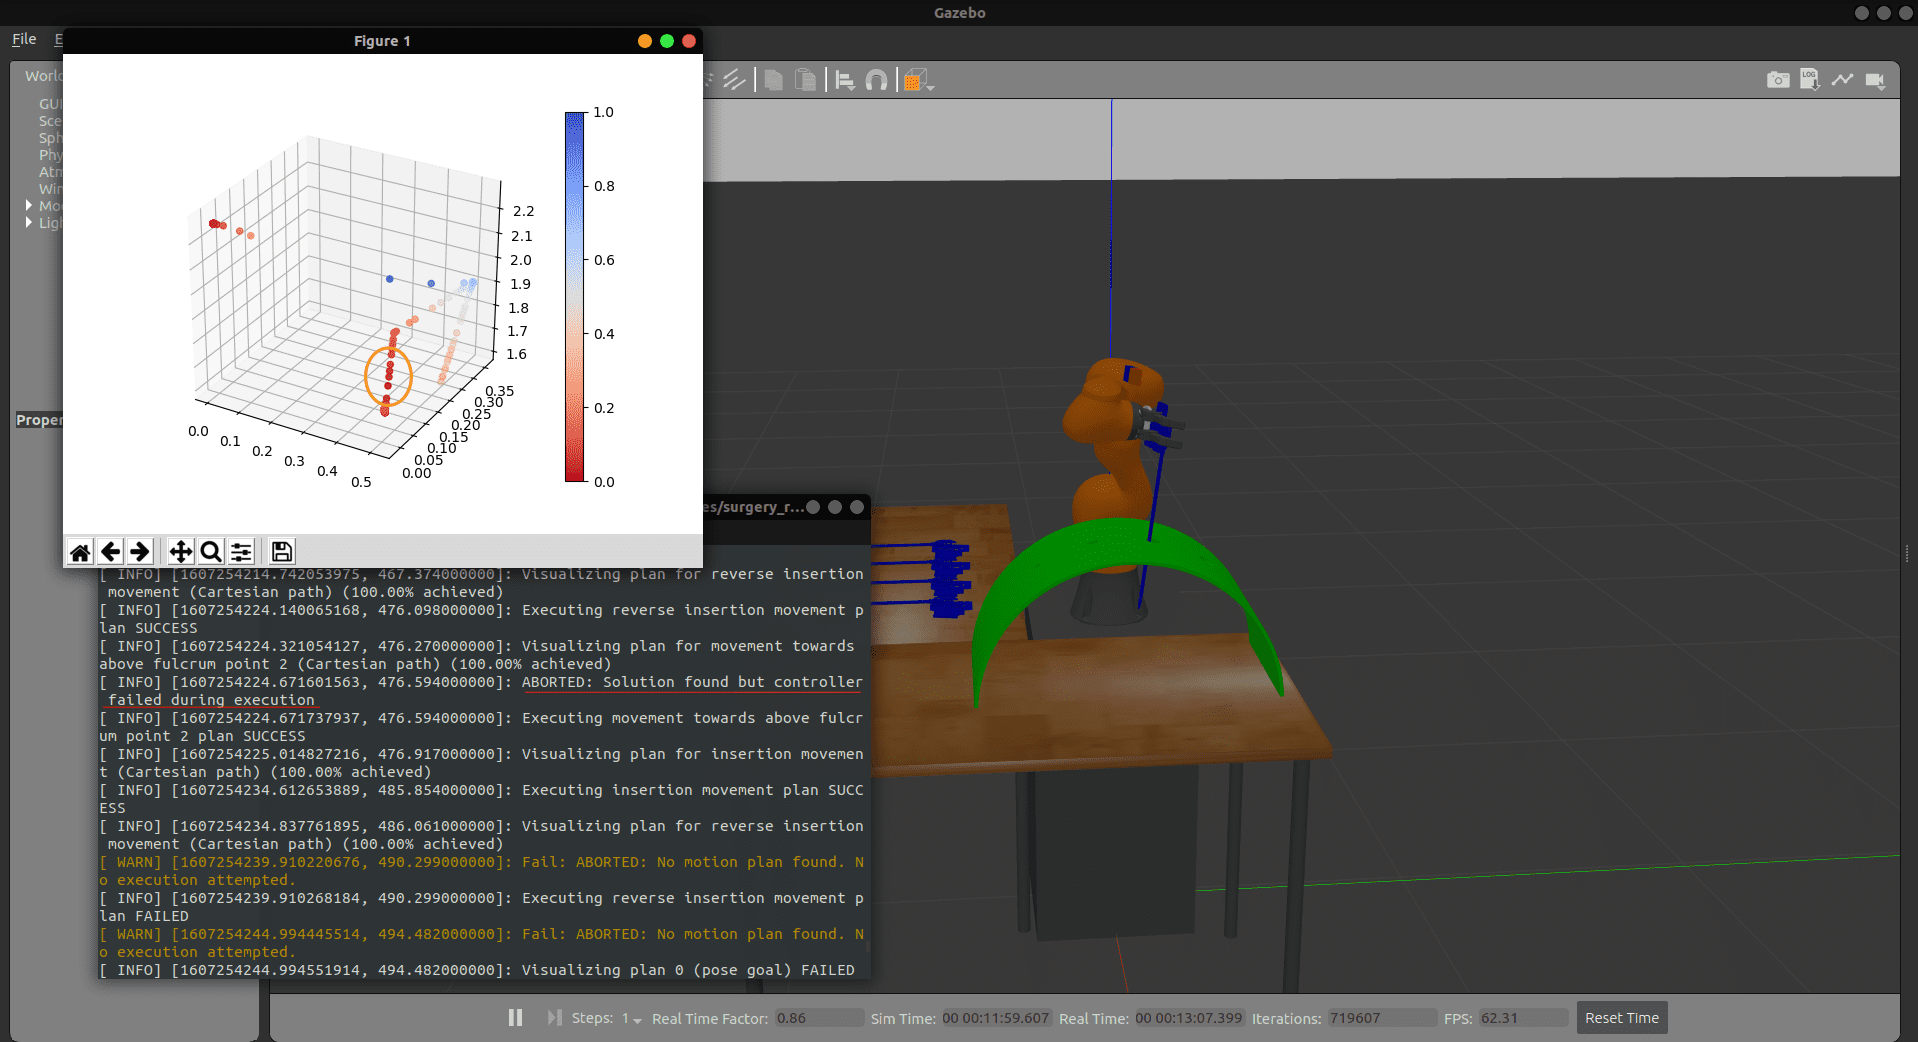
\includegraphics[width=0.9\textwidth]{images/robot_planner2b/singularity_failure.png}
\caption{Experiment 2b: Singularity failure}
\end{figure}
\end{center}


\section{Robot Planner 3: Trajectory planning}

The goal of this third experiment is to design and test only some pivot trajectories. The pivot motions follow the equations described in 
\ref{section:pivot-motions}. The trajectories that were designed and tested in this experiments are the following:
\begin{itemize}
\item Circular
\item Arc
\item Line segment
\end{itemize}

\subsection{Circular and Circular arc trajectories in task space}

% Robot Planner 3a with RRTConnect
\begin{table}[H]
\centering
\begin{tabular}{|p{2cm}|c|p{3cm}|p{3cm}|p{3cm}|}
\hline
Robot Planner 3a           & \multicolumn{4}{c}{\textbf{RRTConnect}}                                                                                                 \vline \\
\hline
                          & \multicolumn{4}{c}{\textbf{Place \& Insert tool}}                     \vline \\
\hline
Experiment                & Status & Solution Time & Path Simplification Time & Planning Attempts  \\
\hline
1                         &        &               &                          &  \\
2                         &        &               &                          &  \\
3                         &        &               &                          &  \\
4                         &        &               &                          &  \\
5                         &        &               &                          &  \\
\hline
\textbf{Average} & 	& 	& 	&  \\
\hline
                          & \multicolumn{4}{c}{\textbf{Pivot Trajectory}}                     \vline \\
\hline
Experiment                & Status & Solution Time & Path Simplification Time & Planning Attempts  \\
\hline
1                         &        &               &                          &  \\
2                         &        &               &                          &  \\
3                         &        &               &                          &  \\
4                         &        &               &                          &  \\
5                         &        &               &                          &  \\
\hline
\textbf{Average} & 	& 	& 	&  \\
\hline
\end{tabular}
\caption{Time results for robot planner 3a using the RRTConnect path planner algorithm}
\label{robot-planner3a-rrtconnect-data}
\end{table}


\subsection{Line segment trajectories in task space}

% Robot Planner 3b with RRTConnect
\begin{table}[H]
\centering
\begin{tabular}{|p{2cm}|c|p{3cm}|p{3cm}|p{3cm}|}
\hline
Robot Planner 3b           & \multicolumn{4}{c}{\textbf{RRTConnect}}                                                                                                 \vline \\
\hline
                          & \multicolumn{4}{c}{\textbf{Place \& Insert tool}}                     \vline \\
\hline
Experiment                & Status & Solution Time & Path Simplification Time & Planning Attempts  \\
\hline
1                         &        &               &                          &  \\
2                         &        &               &                          &  \\
3                         &        &               &                          &  \\
4                         &        &               &                          &  \\
5                         &        &               &                          &  \\
\hline
\textbf{Average} & 	& 	& 	&  \\
\hline
                          & \multicolumn{4}{c}{\textbf{Pivot Trajectory}}                     \vline \\
\hline
Experiment                & Status & Solution Time & Path Simplification Time & Planning Attempts  \\
\hline
1                         &        &               &                          &  \\
2                         &        &               &                          &  \\
3                         &        &               &                          &  \\
4                         &        &               &                          &  \\
5                         &        &               &                          &  \\
\hline
\textbf{Average} & 	& 	& 	&  \\
\hline
\end{tabular}
\caption{Time results for robot planner 3b using the RRTConnect path planner algorithm}
\label{robot-planner3b-rrtconnect-data}
\end{table}


\subsection{Cubic Spline trajectories in task space}

% Robot Planner 3c with RRTConnect
\begin{table}[H]
\centering
\begin{tabular}{|p{2cm}|c|p{3cm}|p{3cm}|p{3cm}|}
\hline
Robot Planner 3c           & \multicolumn{4}{c}{\textbf{RRTConnect}}                                                                                                 \vline \\
\hline
                          & \multicolumn{4}{c}{\textbf{Place \& Insert tool}}                     \vline \\
\hline
Experiment                & Status & Solution Time & Path Simplification Time & Planning Attempts  \\
\hline
1                         &        &               &                          &  \\
2                         &        &               &                          &  \\
3                         &        &               &                          &  \\
4                         &        &               &                          &  \\
5                         &        &               &                          &  \\
\hline
\textbf{Average} & 	& 	& 	&  \\
\hline
                          & \multicolumn{4}{c}{\textbf{Pivot Trajectory}}                     \vline \\
\hline
Experiment                & Status & Solution Time & Path Simplification Time & Planning Attempts  \\
\hline
1                         &        &               &                          &  \\
2                         &        &               &                          &  \\
3                         &        &               &                          &  \\
4                         &        &               &                          &  \\
5                         &        &               &                          &  \\
\hline
\textbf{Average} & 	& 	& 	&  \\
\hline
\end{tabular}
\caption{Time results for robot planner 3c using the RRTConnect path planner algorithm}
\label{robot-planner3c-rrtconnect-data}
\end{table}


\subsection{B-Spline trajectories in task space}

% Robot Planner 3d with RRTConnect
\begin{table}[H]
\centering
\begin{tabular}{|p{2cm}|c|p{3cm}|p{3cm}|p{3cm}|}
\hline
Robot Planner 3d           & \multicolumn{4}{c}{\textbf{RRTConnect}}                                                                                                 \vline \\
\hline
                          & \multicolumn{4}{c}{\textbf{Place \& Insert tool}}                     \vline \\
\hline
Experiment                & Status & Solution Time & Path Simplification Time & Planning Attempts  \\
\hline
1                         &        &               &                          &  \\
2                         &        &               &                          &  \\
3                         &        &               &                          &  \\
4                         &        &               &                          &  \\
5                         &        &               &                          &  \\
\hline
\textbf{Average} & 	& 	& 	&  \\
\hline
                          & \multicolumn{4}{c}{\textbf{Pivot Trajectory}}                     \vline \\
\hline
Experiment                & Status & Solution Time & Path Simplification Time & Planning Attempts  \\
\hline
1                         &        &               &                          &  \\
2                         &        &               &                          &  \\
3                         &        &               &                          &  \\
4                         &        &               &                          &  \\
5                         &        &               &                          &  \\
\hline
\textbf{Average} & 	& 	& 	&  \\
\hline
\end{tabular}
\caption{Time results for robot planner 3d using the RRTConnect path planner algorithm}
\label{robot-planner3a-rrtconnect-data}
\end{table}


\subsection{Polynomial trajectories in joint space}

\subsection{Trajectories in joint space with trapezoidal velocity profile}

\subsection{Trajectories in joint space with s-curve velocity profile}

\section{Robot Planner 4: Simple cube pick-and-place experiment}

In this experiment we plan a simple pick-and-place path for a cube. The robotic arm first visits the left table and starts from the pre-grasp posture and then 
slowly approaches the cube until the grasp posture. When the gripper has reached the grasp posture, it closes the fingers to grasp the object and then retreats 
to the post-grasp posture. After that the robotic arm visits the right table to execute the place steps which are similar to the pick steps. The images below 
show some frames from the experiment with the first three to show the pick steps in the simulation environment and then other three images show the place steps 
in the visualization program.

\begin{center}
\begin{figure}[H]
\centering
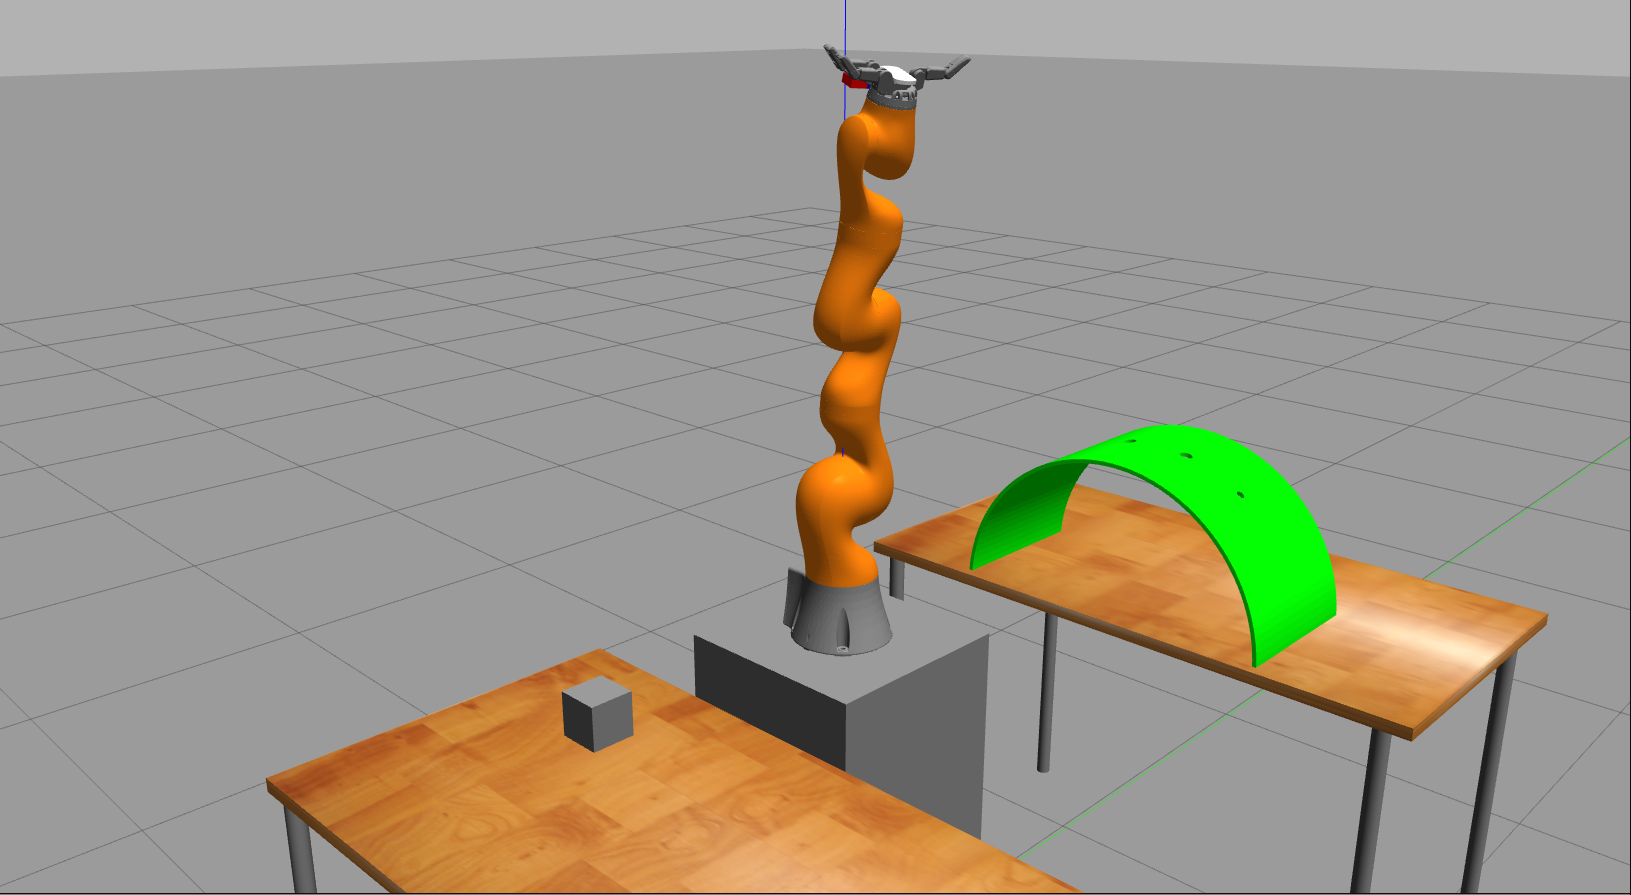
\includegraphics[width=0.3\textwidth]{images/robot_planner4/robot_planner4_1}
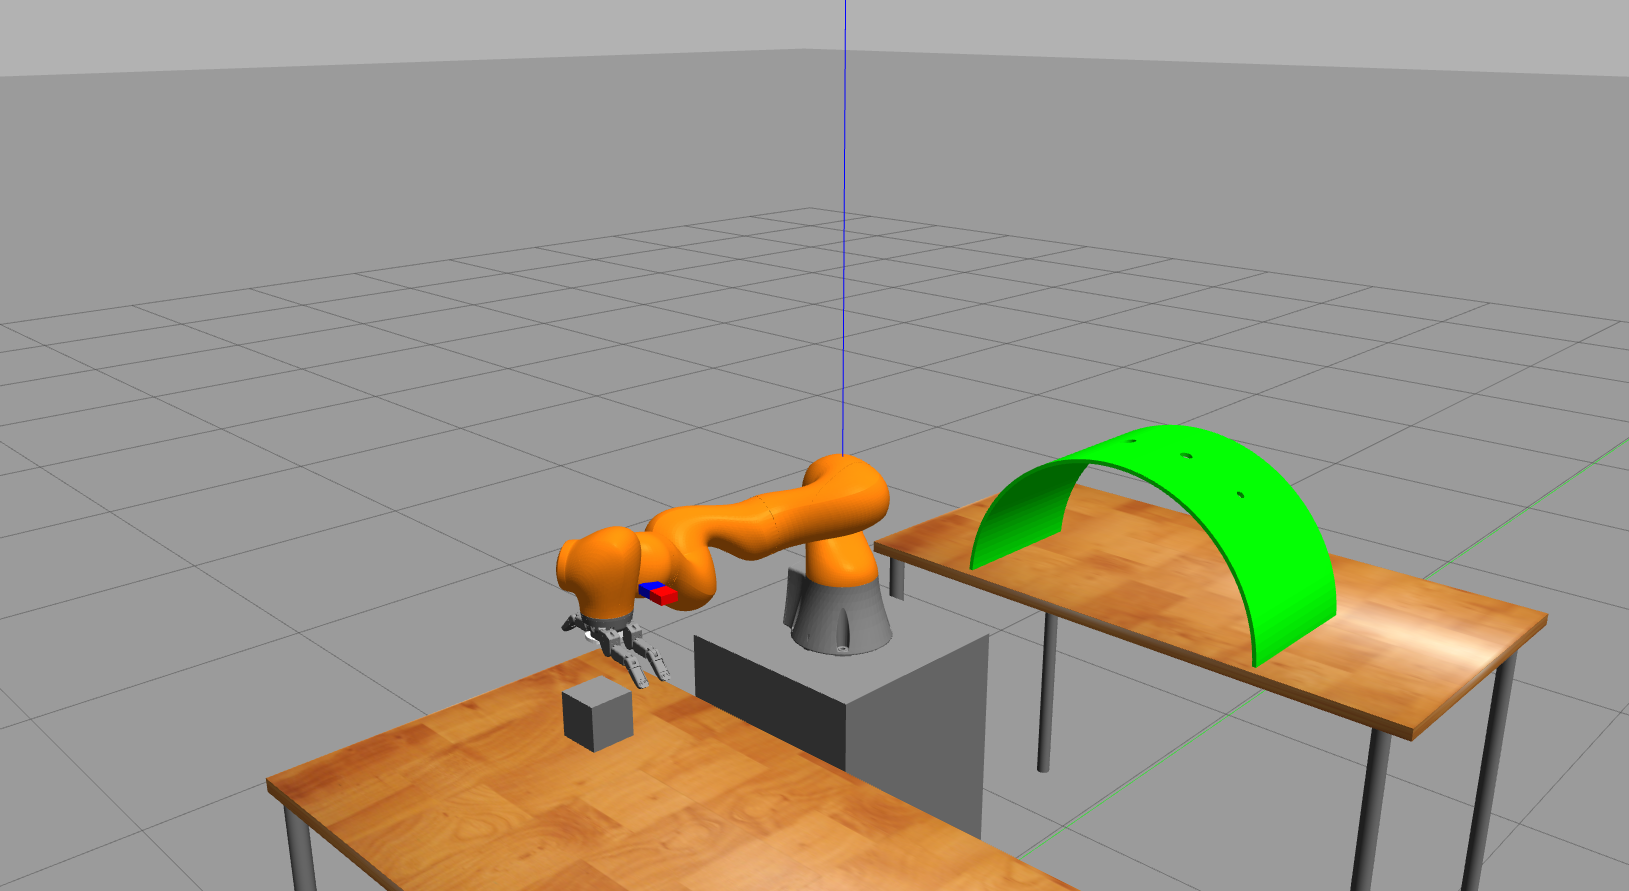
\includegraphics[width=0.3\textwidth]{images/robot_planner4/robot_planner4_3}
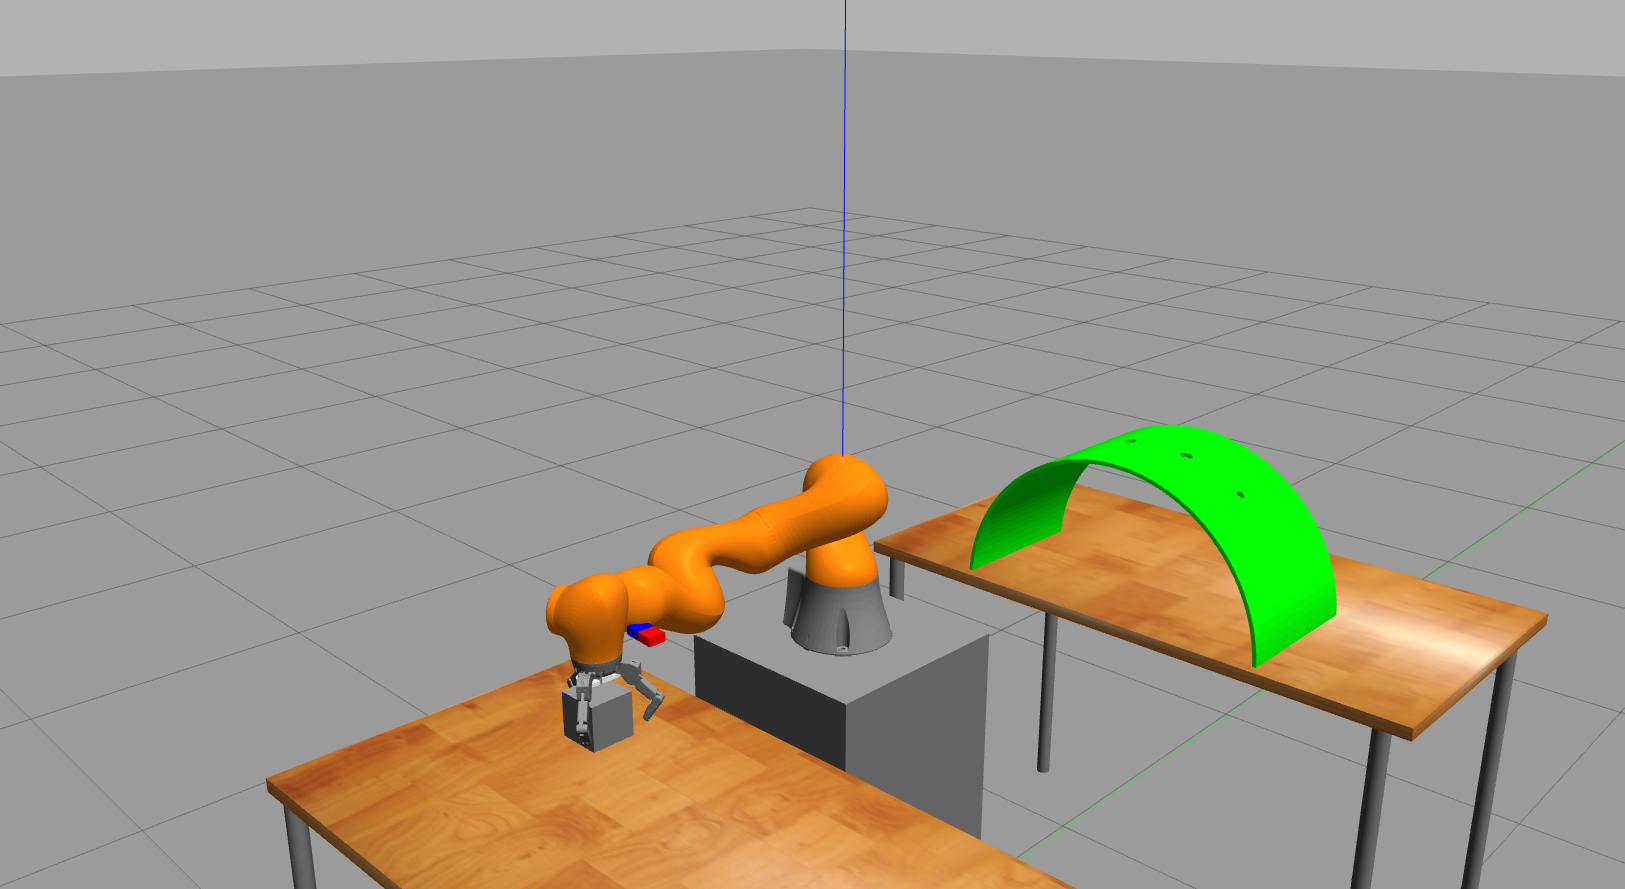
\includegraphics[width=0.3\textwidth]{images/robot_planner4/robot_planner4_5}\\
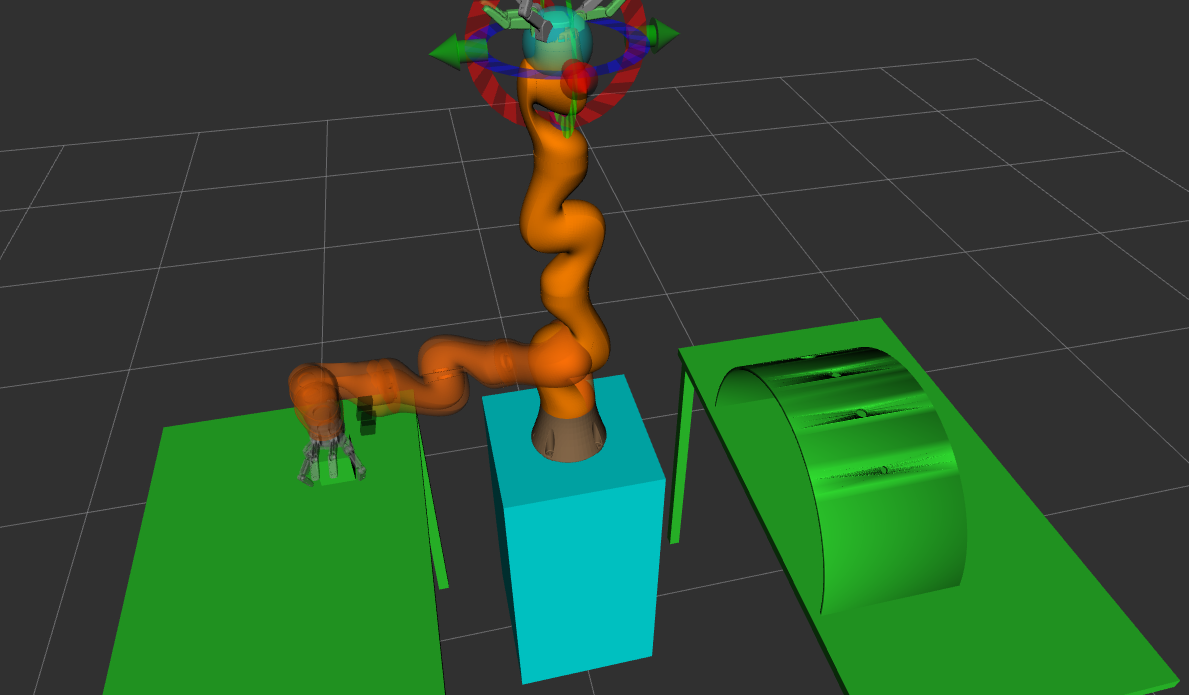
\includegraphics[width=0.3\textwidth]{images/robot_planner4/robot_planner4_6}
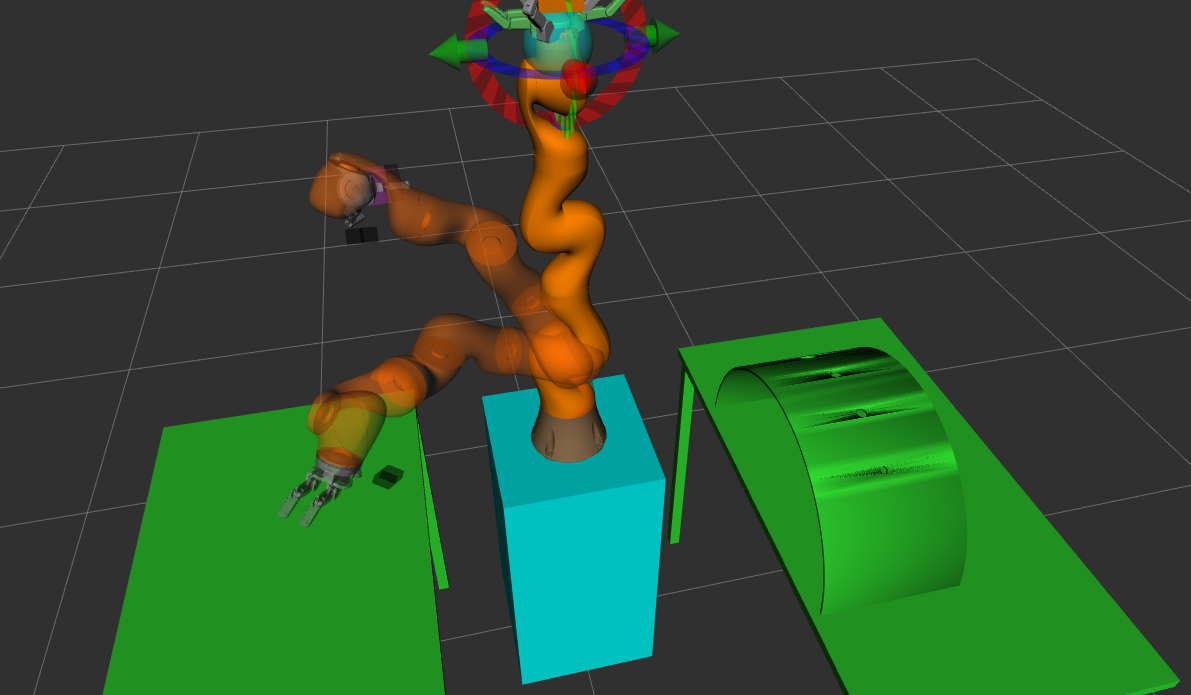
\includegraphics[width=0.3\textwidth]{images/robot_planner4/robot_planner4_8}
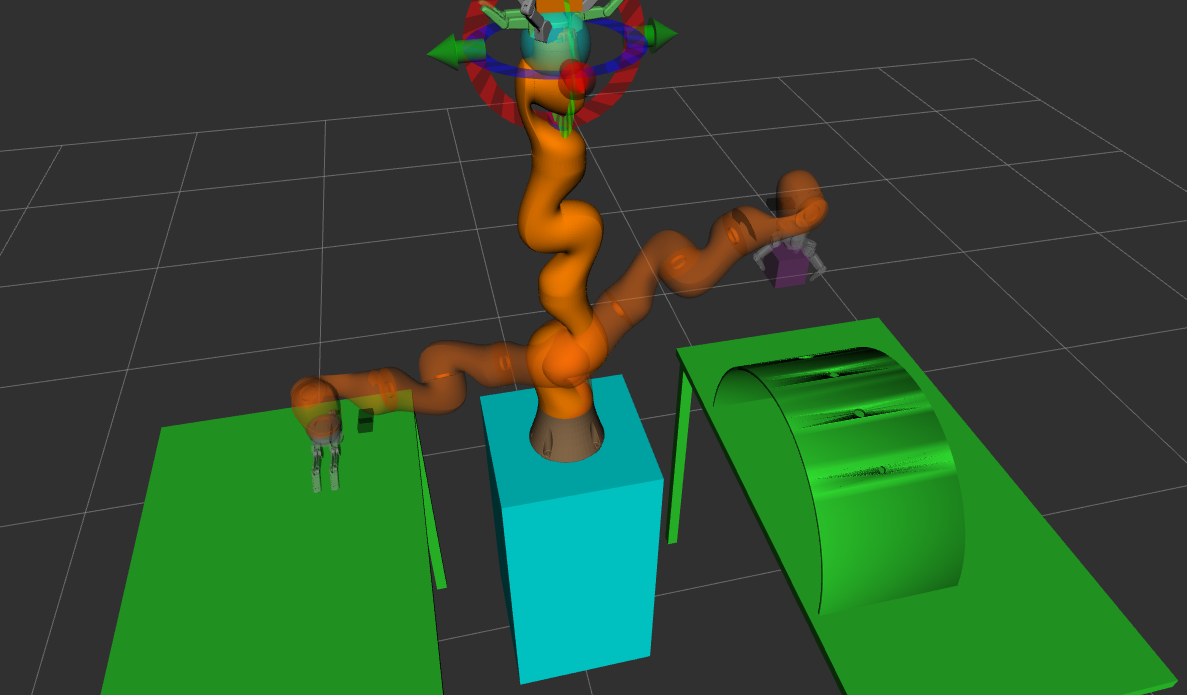
\includegraphics[width=0.3\textwidth]{images/robot_planner4/robot_planner4_10}\\
\caption{Experiment 4: Simple pick-and-place experiment of a cube}
\end{figure}
\end{center}

Observing the results from table \ref{robot-planner4-rrtconnect-data}, the time duration for the pick pipeline of this experiment using the RRTConnect path planning algorithm, 
ranges from approximately 0.01 to 0.02 seconds, whereas in the Place pipeline we observe mainly 2 distinct groups of time ranges. One group has values around 0.02 seconds and the other 
has bigger values around 0.14 seconds. In the case with the bigger time durations, the solution made the robot go around the obstacle whereas in the other cases the path planning solution avoided the obstacle, 
which means that an easier path was found, it was solved quicker and the path solution was much simpler (in terms of kinematic constraints) which led to smaller path simplification time durations. 
It is also possible, that due to the obstacle and the initial conditions, the robot may not find a solution at the first attempt or none at all.

% Robot Planner 4 with RRTConnect
\begin{table}[H]
\centering
\begin{tabular}{|p{2cm}|c|p{3cm}|p{3cm}|p{3cm}|}
\hline
Robot Planner 4           & \multicolumn{4}{c}{\textbf{RRTConnect}}                                                                                                 \vline \\
\hline
                          & \multicolumn{4}{c}{\textbf{Pick Pipeline}}                     \vline \\
\hline
Experiment                & Status & Solution Time & Path Simplification Time & Planning Attempts  \\
\hline
1 & 1 & 0.026189 & 0.065173 & 1 \\
2 & 1 & 0.016835 & 0.043333 & 1 \\
3 & 1 & 0.025439 & 0.023178 & 1 \\
4 & 1 & 0.029292 & 0.066913 & 1 \\
5 & 1 & 0.024873 & 0.01747 & 1 \\
6 & 1 & 0.017615 & 0.024568 & 1 \\
7 & 1 & 0.014263 & 0.028095 & 1 \\
8 & 1 & 0.015479 & 0.027035 & 1 \\
9 & 1 & 0.027803 & 0.057064 & 1 \\
10 & 1 & 0.026057 & 0.033179 & 1 \\
\hline
\textbf{Average} & 1	& 0.02196178	& 0.0386008	& 1 \\
\hline
                          & \multicolumn{4}{c}{\textbf{Place Pipeline}}                     \vline \\
\hline
Experiment                & Status & Solution Time & Path Simplification Time & Planning Attempts  \\
\hline
1 & 1 & 0.014644 & 0.020947 & 1 \\
2 & 1 & 0.131334 & 0.938948 & 1 \\
3 & 1 & 0.021425 & 0.08429 & 1 \\
4 & 1 & 0.01675 & 0.01675 & 1 \\
5 & 1 & 0.165795 & 1.661019 & 1 \\
6 & 1 & 0.119819 & 0.394493 & 1 \\
7 & 1 & 0.140645 & 0.476835 & 1 \\
8 & 1 & 0.133917 & 0.673233 & 1 \\
9 & 1 & 0.017644 & 0.038319 & 1 \\
10 & 1 & 0.020025 & 0.074847 & 1 \\
\hline
\textbf{Average} & 1	& 0.0781998	& 0.4379681	& 1 \\
\hline
\end{tabular}
\caption{Time results for robot planner 4 using the RRTConnect path planner algorithm}
\label{robot-planner4-rrtconnect-data}
\end{table}

The main observation from the results of table \ref{robot-planner4-rrtstar-data} is that RRT* time durations are much bigger than those from RRTConnect, but the RRT* algorithm has the advantage of finding better, more accurate solutions (approximately the same solutions at most attempts) and with less collisions. Although these time durations are not optimal for real-time applications, they could be useful in pick-and-place pipelines 
if the solutions are pre-computed (memoized) and saved for later use.

% Robot Planner 4 with RRT*
\begin{table}[H]
\centering
\begin{tabular}{|p{2cm}|c|p{3cm}|p{3cm}|p{3cm}|}
\hline
Robot Planner 4           & \multicolumn{4}{c}{\textbf{RRT*}}                                                                                                 \vline \\
\hline
                          & \multicolumn{4}{c}{\textbf{Pick Pipeline}}                     \vline \\
\hline
Experiment                & Status & Solution Time & Path Simplification Time & Planning Attempts  \\
\hline
1	& 1 & 44.97476	& 0.030918	& 1	\\
2	& 1 & 45.006897	& 0.073009	& 1	\\
3	& 1	& 44.989085	& 0.053440	& 1	\\
4	& 1 & 44.998414	& 0.034571	& 1	\\
5	& 1 & 44.982524	& 0.041732	& 1	\\
6	& 1 & 44.997148	& 0.017660	& 1	\\
7	& 1 & 45.00115	& 0.022290	& 1	\\
8	& 1 & 44.991409	& 0.046728	& 1	\\
\hline
\textbf{Average} & 1 & 44.99267	& 0.0400435	& 1	\\
\hline
                          & \multicolumn{4}{c}{\textbf{Place Pipeline}}                     \vline \\
\hline
Experiment                & Status & Solution Time & Path Simplification Time & Planning Attempts  \\
\hline
1	& 1	& 45.064568	& 0.884821	& 1 \\
2	& 1	& 44.965931	& 0.054692	& 1 \\
3	& 1	& 44.976697	& 0.012784	& 1 \\
4	& 1	& 44.968431	& 0.020354	& 1 \\
5	& 1	& 45.068239	& 0.551800	& 1 \\
6	& 1	& 45.016043	& 1.089529	& 1 \\
7	& 1	& 45.048851	& 0.680121	& 1 \\
8	& 1	& 45.023364	& 0.000004	& 1 \\
\hline
\textbf{Average} & 1	& 45.0165155	& 0.411763	& 1 \\
\hline
\end{tabular}
\caption{Time results for robot planner 4 using the RRT* path planner algorithm}
\label{robot-planner4-rrtstar-data}
\end{table}

% Robot Planner 4 with PRM*
\begin{table}[H]
\centering
\begin{tabular}{|p{2cm}|c|p{3cm}|p{3cm}|p{3cm}|}
\hline
Robot Planner 4           & \multicolumn{4}{c}{\textbf{PRM*}}                                                                                                 \vline \\
\hline
                          & \multicolumn{4}{c}{\textbf{Pick Pipeline}}                     \vline \\
\hline
Experiment                & Status & Solution Time & Path Simplification Time & Planning Attempts  \\
\hline
1	& 1	& 44.987182	& 0.000028	& 1 \\
2	& 1	& 44.992757	& 0.000005	& 1 \\
3	& 1	& 45.00983	& 0.000004	& 1 \\
4	& 1	& 45.004154	& 0.105568	& 1 \\
5	& 1	& 44.99367	& 0.000002	& 1 \\
6	& 1	& 45.015169	& 0.000002	& 1 \\
7	& 1	& 45.02914	& 0.000002	& 1 \\
\hline
\textbf{Average} & 1	& 45.00456	& 0.015088	& 1 \\
\hline
                          & \multicolumn{4}{c}{\textbf{Place Pipeline}}                     \vline \\
\hline
Experiment                & Status & Solution Time & Path Simplification Time & Planning Attempts  \\
\hline
1	& 1	& 44.992207	& 0.000004	& 1 \\
2	& 1	& 45.512132	& 0.000001	& 1 \\
3	& 1	& 45.950533	& 0.000002	& 1 \\
4	& 1	& 44.99777	& 0.000003	& 1 \\
5	& 1	& 45.691226	& 0.000002	& 1 \\
6	& 1	& 45.023251	& 0.013478	& 1 \\
7	& 1	& 45.782305	& 0.000003	& 1 \\
\hline
\textbf{Average}	& 1	& 45.421346	& 0.0019276	& 1 \\
\hline
\end{tabular}
\caption{Time results for robot planner 4 using the PRM* path planner algorithm}
\label{robot-planner4-prmstar-data}
\end{table}


\section{Robot Planner 5: Visual servoing}

The goal of this fifth experiment is to control the KUKA robot using the camera via the visual servoing technique. In the first part of the experiment the 
robotic arm goes to an initial known position (e.g. the corner of the table) and then moves around until it detects a surgical tool. When that happens, the 
image-based visual servoing will send commands to the robot so that the detected tool is at the center of the video frame and with the same orientation 
as the video frame. At the second part of the experiment, the robot follows a similar algorithm. It starts with a known position, like the corner of the second 
table, then moves around until the mounting dock starts to appear inside the frame. When that happens, the image-based visual servoing will send commands to the 
robot so that the center of the trocar or the fulcrum reference frame is at the center and with the same orientation as the video frame. Similar results can be 
achieved by using position-based visual servoing, but that was not chosen at this implementation for simplicity and less operations. Position-based servoing 
requires more calculations because it is required to get the camera's transformation, express it with respect to the end-effector and then calculate the 
end-effector pose which is then used as an input to a Cartesian Controller.

\begin{center}
\begin{figure}[H]
\centering
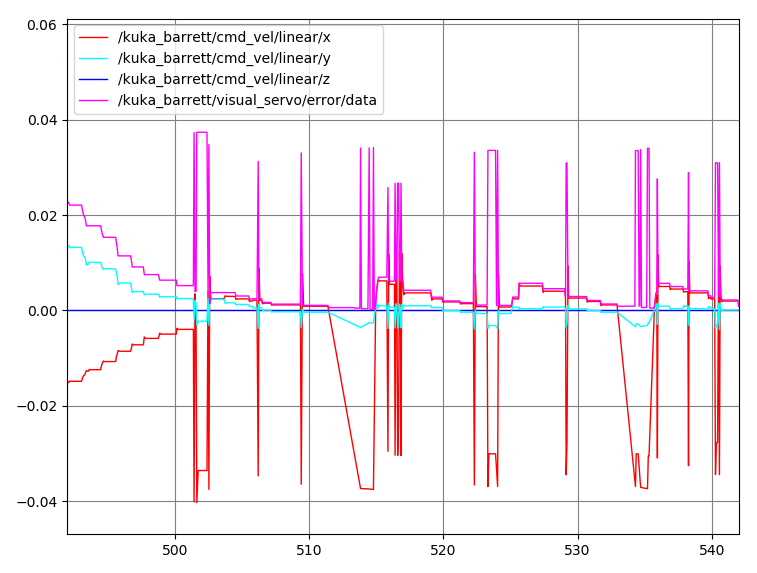
\includegraphics[width=0.45\textwidth]{images/robot_planner5/visual_servo_controller3.png}
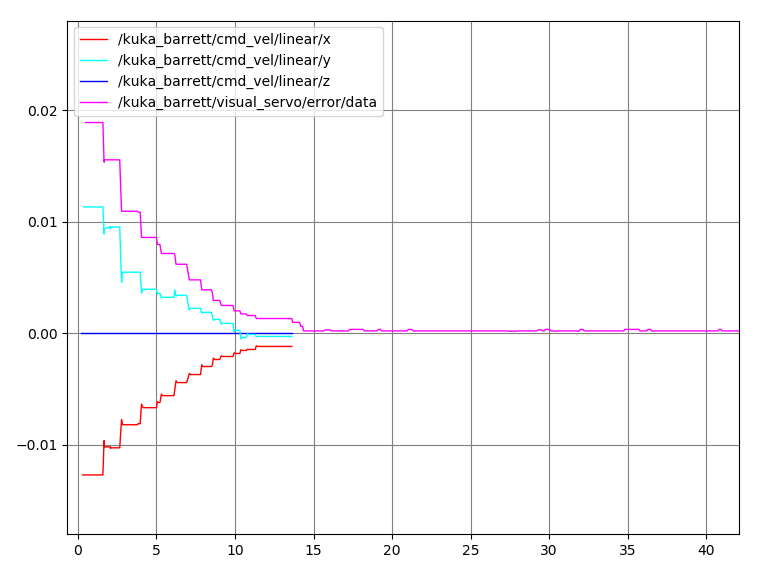
\includegraphics[width=0.45\textwidth]{images/robot_planner5/visual_servo_controller4.png}\\
\caption{Visual servo controller error diagrams. On the left image in the error graphs appear some spikes. These spikes occur from the sudden temporary detection 
of a nearby surgical tool. On the right image, these spikes are filtered out, and only the error graphs of the visual servoing of one tool are shown. The  
controller parameters are $K_p = 0.9, K_d = 0.2$}
\end{figure}
\end{center}

\begin{center}
\begin{figure}[H]
\centering
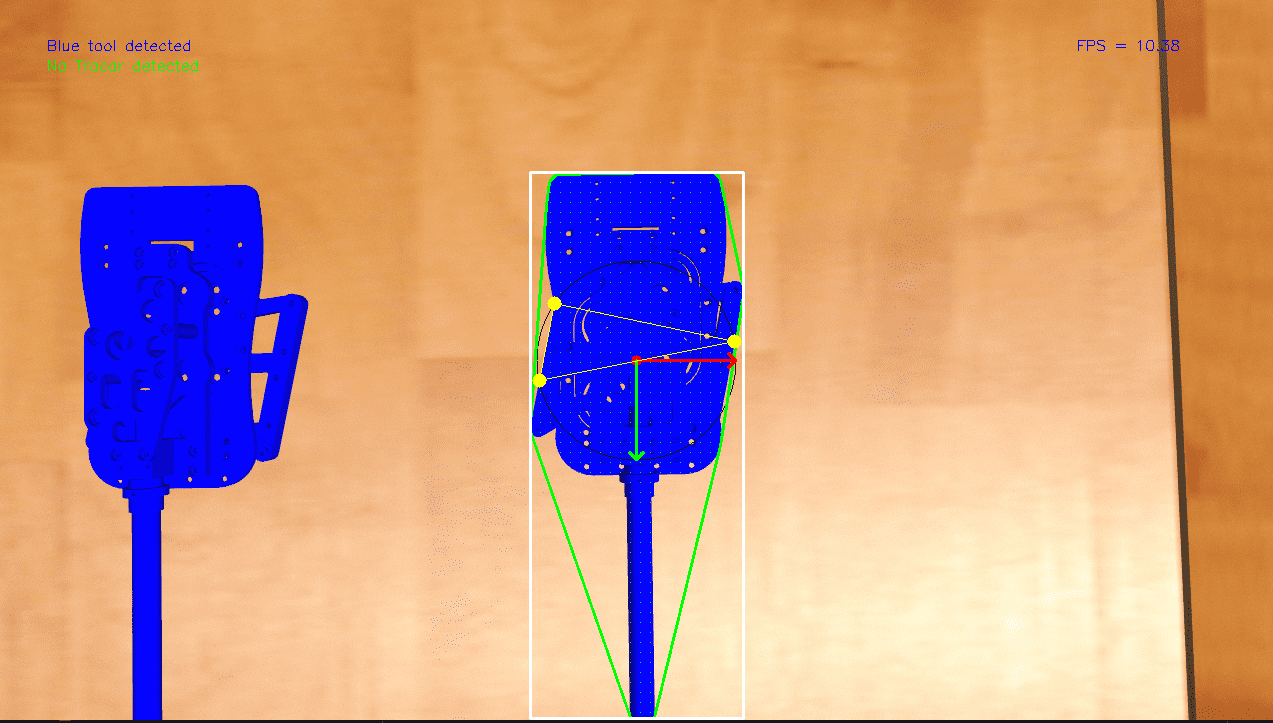
\includegraphics[width=0.6\textwidth]{images/grasp-points-triangle.png}\\
\caption{Image based visual servoing and calculation of grasp points. The yellow points are the grasp points and the thin black circumscribed circle is the growing circle that was used to calculate them.}
\end{figure}
\end{center}

\section{Robot Planner 6}

\section{Robot Planner 7}

\section{Robot Planner 8: State machine \& ROS Actions}